\documentclass[11pt,a4paper]{report}\usepackage[]{graphicx}\usepackage[]{color}
%% maxwidth is the original width if it is less than linewidth
%% otherwise use linewidth (to make sure the graphics do not exceed the margin)
\makeatletter
\def\maxwidth{ %
  \ifdim\Gin@nat@width>\linewidth
    \linewidth
  \else
    \Gin@nat@width
  \fi
}
\makeatother

\definecolor{fgcolor}{rgb}{0.345, 0.345, 0.345}
\newcommand{\hlnum}[1]{\textcolor[rgb]{0.686,0.059,0.569}{#1}}%
\newcommand{\hlstr}[1]{\textcolor[rgb]{0.192,0.494,0.8}{#1}}%
\newcommand{\hlcom}[1]{\textcolor[rgb]{0.678,0.584,0.686}{\textit{#1}}}%
\newcommand{\hlopt}[1]{\textcolor[rgb]{0,0,0}{#1}}%
\newcommand{\hlstd}[1]{\textcolor[rgb]{0.345,0.345,0.345}{#1}}%
\newcommand{\hlkwa}[1]{\textcolor[rgb]{0.161,0.373,0.58}{\textbf{#1}}}%
\newcommand{\hlkwb}[1]{\textcolor[rgb]{0.69,0.353,0.396}{#1}}%
\newcommand{\hlkwc}[1]{\textcolor[rgb]{0.333,0.667,0.333}{#1}}%
\newcommand{\hlkwd}[1]{\textcolor[rgb]{0.737,0.353,0.396}{\textbf{#1}}}%
\let\hlipl\hlkwb

\usepackage{framed}
\makeatletter
\newenvironment{kframe}{%
 \def\at@end@of@kframe{}%
 \ifinner\ifhmode%
  \def\at@end@of@kframe{\end{minipage}}%
  \begin{minipage}{\columnwidth}%
 \fi\fi%
 \def\FrameCommand##1{\hskip\@totalleftmargin \hskip-\fboxsep
 \colorbox{shadecolor}{##1}\hskip-\fboxsep
     % There is no \\@totalrightmargin, so:
     \hskip-\linewidth \hskip-\@totalleftmargin \hskip\columnwidth}%
 \MakeFramed {\advance\hsize-\width
   \@totalleftmargin\z@ \linewidth\hsize
   \@setminipage}}%
 {\par\unskip\endMakeFramed%
 \at@end@of@kframe}
\makeatother

\definecolor{shadecolor}{rgb}{.97, .97, .97}
\definecolor{messagecolor}{rgb}{0, 0, 0}
\definecolor{warningcolor}{rgb}{1, 0, 1}
\definecolor{errorcolor}{rgb}{1, 0, 0}
\newenvironment{knitrout}{}{} % an empty environment to be redefined in TeX

\usepackage{alltt}
\setlength{\parindent}{4ex}
\setlength{\parskip}{1ex}
\renewcommand{\baselinestretch}{1.8}
\usepackage[english]{babel}
\usepackage[latin1]{inputenc}
\usepackage[T1]{fontenc}
\usepackage[a4paper,top=3cm,bottom=3cm,left=3cm,right=3cm,marginparwidth=1.75cm]{geometry}
\usepackage{titlesec}
\usepackage{amsmath}
\usepackage{amsthm}
\usepackage{footnote}
\usepackage{tablefootnote}
\usepackage{amsfonts}
\usepackage{graphicx}
\usepackage{geometry}
\usepackage{wrapfig}
\usepackage{float}
\usepackage{mathtools}
\usepackage{epsfig}
\usepackage{apacite}
\usepackage{natbib}
\usepackage{caption}
\usepackage{subfig}
\usepackage[toc,page]{appendix}
\usepackage[export]{adjustbox}
\usepackage[linesnumbered,lined,boxed,commentsnumbered]{algorithm2e} 
\usepackage{setspace}
\usepackage{tikz}
\usepackage{color}
\usepackage{pdflscape}
\usepackage{afterpage}
\usetikzlibrary{arrows,calc,positioning, decorations.pathreplacing}
\tikzstyle{vertex}=[auto=left,circle,fill=black!25,minimum size=20pt,inner sep=0pt]
\definecolor{dodgerblue}{rgb}{0.06,0.30,0.54}
\definecolor{red3}{rgb}{0.8,0.07,0.12}


\newtheorem{theorem}{Theorem}[section]
\newtheorem{lemma}{Lemma}[section]
\newtheorem{property}{Property}[section]
\newtheorem{proposition}{Proposition}[section]
\IfFileExists{upquote.sty}{\usepackage{upquote}}{}
\begin{document}

% Turn off page numbering until first section.
\pagenumbering{gobble}

% Title page - needs Stats_Logo.png
\begin{titlepage}
\begin{center}
\vspace{1cm}
\textsf{\Huge{University of Oxford \\}}
\vspace{1cm}
\begin{figure}[htb]
\centering

\includegraphics[scale=.8]{logo.png}
\end{figure}
\vspace{2.0cm}
\Huge{Approximate inference for large data sets in a sample Bayesian setting\\}
\vspace{2.0cm}
\large{ by \\[14pt] Adrien Bec-Hairault \\[8pt] Green Templeton College} \\
\vspace{2.2cm}
\large{A dissertation submitted in partial fulfilment of the degree of Master of Science in Statistical Science.} \\
\vspace{.5cm}
\large{\emph{Department of Statistics, 24--29 St Giles, \\Oxford, OX1 3LB}} \\
\vspace{1.0cm}
\large{September 2018} \\
\end{center}
\end{titlepage}
\clearpage

This is my own work (except where otherwise indicated).
\vspace{2.5in}

\begin{center}
Candidate: Adrien Hairault\\
\vspace{1.0in}
Signed:.................................\\
\vspace{1.0in}
Date:...................................
\end{center}
\clearpage
\begin{abstract}

The use of classic Monte Carlo Markov Chains (MCMC) algorithms in the context of Bayesian inference, which usually involves repeated likelihood evaluations, has become more and more computationally expensive with the advent of Big Data. This dissertation assesses and compares the efficiency of five recent algorithms designed to respond to this challenge. First, we review extensively the theory behind each algorithm, provide a potential pseudo-code implementation, and identify mistakes in two of the original articles, one of which seems substantial. Second, we test the algorithms on different synthetic data sets to reveal their strengths and weaknesses. Among other techniques, the key metrics we use are the Effective Sample Size (ESS) per likelihood evaluation (for efficiency) as well as the quality of the posterior approximation, measured by the Hellinger distance between the desired target and the obtained output.
\end{abstract}
\clearpage
%\thispagestyle{empty}
\vspace*{2in}
\begin{center}
\textbf{Acknowledgements}
\end{center}

I would like to thank my dissertation supervisor Geoff Nicholls for his patient and helpful guidance. Thank you for having answered so promptly all my questions and queries and for coming up with great ideas.\\
I would also like to thank my mother, Fr\'ed\'erique Bec, for the moral support and the help she gave me during the proof-reading process.\\
Thank you Olga Kosno, my dear friend, so far and yet so close.\\
Finally, completing this dissertation and this year in Oxford would certainly have been harder without the help of the wonderful persons I have met and whom I know I will meet again.\\

\clearpage



\tableofcontents
\pagenumbering{arabic}

\chapter*{Introduction}
\addcontentsline{toc}{chapter}{Introduction}
\label{sec:intro}

Both frequentist and Bayesian approaches of inference assume that for any parameter $\theta$ there exists a true value $\theta_0$. However, Bayesian inference regards parameter $\theta$ as a random variable, which is not conceivable in a frequentist framework. The \textit{posterior} distribution of parameter $\theta$, cornerstone of Bayesian analysis, updates thanks to Bayes' formula\footnote{The Bayes' theorem, derived by Thomas Bayes (1701-1761) and Pierre-Simon Laplace (1749-1827), states that for any events $A$ and $B$ such that $P(B)\neq 0$, $$P(A|B)=\frac{P(B|A)P(A)}{P(B)}$$} the prior knowledge of the scientist about $\theta$, embodied by a \textit{prior} distribution, with the information about the parameter carried by the data, given by the \textit{likelihood} distribution. In short, 
\begin{align}
\label{eq:bayes}
    \pi(\theta|z)&=\frac{p(z|\theta)\pi(\theta)}{\int_{\theta\in\Theta} p(z|\theta)\pi(\theta)d\theta}\\
    &\propto p(z|\theta)\pi(\theta)\nonumber
\end{align}
where, $z$, $\pi(.|z)$, $\pi(.)$, $p(.|\theta)$, $\Theta$ denote respectively the data, the posterior and the prior distributions of $\theta$, the likelihood function, and the parameter space.\\
Hence, in a Bayesian inference framework, the posterior distribution can be seen as a measure of uncertainty, or a strength of belief about the true value of parameter $\theta$\\
However, in practice, this distribution is usually intractable and measures of interest like its mean or mode may not be derived analytically, leading to the dominance of frequentist methods over Bayesian ones in the first half of the 20th century. The emergence of Monte Carlo Markov Chains (MCMC) with the Metropolis-Hastings (MH) algorithm by \cite{metropolis1953equation} coupled with the advent of powerful computers enabled a strong resurgence of Bayesian analysis. This fairly simple algorithm allows sampling from any distribution provided one can evaluate its probability density function up to a normalising constant. We give below a possible implementation of the random walk Metropolis Hastings algorithm.

\begin{center}
\begin{algorithm}[H]
\setstretch{1}
\caption{\texttt{Metropolis-Hastings}}
\label{algo:MH}
\SetKwInOut{Input}{Input}
\SetKwInOut{Output}{Output}
\Input{data set $z$, number of samples $T$, initial state $\theta_0$, proposal distribution $q$}
\Output{$\{\theta_t\}_{t=0}^T$ asymptotically from $\pi(\theta|z)\propto p(z|\theta)\pi(\theta)$}
Initialization\;
$llik_{current}\leftarrow p(z|\theta_0)$\;
\For{t=0,...,T}{
$\theta'\sim q(.|\theta_t)$\;
$llik_{proposal}\leftarrow p(z|\theta')$\;
$u\sim\mathcal U_{[0,1]}$\;
$\alpha\leftarrow\min(1,\frac{llik_{proposal}\pi(\theta')q(\theta_t|\theta')}{llik_{current}\pi(\theta_t)q(\theta'|\theta_t)})$\;
\eIf{$u\leq\alpha$}{
$\theta_{t+1}\leftarrow\theta'$\;
$llik_{current}\leftarrow llik_{proposal}$
}
{
$\theta_{t+1}\leftarrow\theta_t$
}
}
\end{algorithm}
\end{center}

Among other methods, Monte Carlo Markov Chains (MCMC) algorithms have been used for years in order to approximate any posterior distribution in the context of Bayesian inference. However, repeated evaluations of the likelihood function, which are at the core of the vast majority of MCMC algorithms (cf algorithm \ref{algo:MH}), have become more and more computationally expensive with the recent and steady increase in size of data sets, also known as Big Data.\\
This dissertation aims at reviewing five recent MCMC methods designed to bypass likelihood evaluations on the full data set in order to reduce the high computational cost inherent to the implementation of classic MCMC methods. The diverse choice of algorithms reviewed reflects our desire to cover a broad part of the spectrum of current research in this field of statistics. Using \cite{bardenet2017markov}'s terminology, we may classify those algorithms as falling into two categories.
Among the \textit{Divide-and-conquer approaches} we present \textit{Consensus Monte Carlo} by \cite{scott2016bayes} and the \textit{Non-Parametric Density Product Estimator} (NPDPE) by \cite{neiswanger2013asymptotically}.
The other algortihms we review fall into the \textit{subsampling methods} category, namely a \textit{Pseudo-Marginal} (PM) algorithm by \cite{quiroz2018speeding}, a \textit{rejection-free} stochastic-gradient method by \cite{welling2011bayesian} which builds upon Langevin Dynamics (SGLD), and the \textit{Approximate Metropolis-Hastings test} (ApMHT) by \cite{korattikara2014austerity}. \\

In Chapter \ref{chap:algorithms} we review extensively each method explaining the mechanisms at work and providing our pseudo-code implementation. We also report the proofs of interest and complete them by filling out the gaps left intentionally by the authors or by showing some properties left unproved. Furthermore, after spotting a mistake in an essential consistency proof of algorithm ApMHT, we provide a corrected alternative that leads to the desired result.\\
In Chapter \ref{chap:eperiments} we explain in details our methodology and assessment criteria before confronting our algorithms to four synthetic Bayesian models whose posteriors display features such as multi-modality, high variance and high dimensionality. We then sum up our discoveries and the limitations of our analysis.
\newpage
\chapter{Algorithms}
In this section, we attempt to make notation consistent across the five articles of interest.\\
Therefore, $q(\theta'|\theta), p(z|\theta),\pi(\theta|z)$ and $\pi(\theta)$ will denote respectively the proposal distribution used in the algorithm, the likelihood function, the posterior and the prior distributions. We also let $z$ be a data set of size $N$ and $\theta$ a parameter in $\Theta\subset\mathbb R^d$.
\label{chap:algorithms}
\section{Approximate Metropolis-Hastings Test (ApMHT)}
\label{sec:korattikara_exp}
We now present the first of the algorithms we review in this dissertation.
\cite{korattikara2014austerity} propose an interesting alternative to evaluating the likelihood function on the whole data set.\\
Suppose that the observations are conditionally independent given the parameter $\theta$, i.e that $p(z|\theta)=\prod_{i=1}^Np(z_i|\theta)$, then the posterior distribution can be written as follows.
$$\pi(\theta|z)\propto\pi(\theta)\prod_{i=1}^Np(z_i|\theta)$$

\noindent We prove the following proposition that is used by \cite{korattikara2014austerity} in order to reformulate the usual MH accept-reject step (cf algorithm \ref{algo:MH})
\begin{proposition}
\label{eq:korattikara1.1}
Let $u\sim\mathcal{U}_{[0,1]}$ and $\alpha=\min\left(1,\frac{\pi(\theta'|z)q(\theta_t|\theta')}{\pi(\theta|z)q(\theta'|\theta_t)}\right)$. Then  $u\leq\alpha\Leftrightarrow\mu_0\leq\mu$, where
\begin{align}
\mu_0&=\frac1N\log\left(u\frac{\pi(\theta_t)q(\theta'|\theta_t)}{\pi(\theta')q(\theta_t|\theta')}\right)\\
\mu&=\frac1N\sum_{i=1}^Nl_i\text{ where }l_i=\log p(z_i|\theta')-\log p(z_i|\theta_t)\text{for $\theta', \theta_t \in \Theta$}
\end{align}
And $\alpha$ denotes the standard Metropolis-Hastings acceptance probability (cf algorithm \ref{algo:MH})
\end{proposition}
\noindent\textit{Proof.}
\begin{align*}
\mu_0\leq\mu&\Leftrightarrow 
\log\left(u\frac{\pi(\theta_t)q(\theta'|\theta_t)}{\pi(\theta')q(\theta_t|\theta')}\right)-\sum_{i=1}^Nl_i\leq 0\\
&\Leftrightarrow \log\left(u\frac{\pi(\theta_t)\prod_{i=1}^Np(z_i|\theta_t)q(\theta'|\theta_t)}{\pi(\theta')\prod_{i=1}^Np(z_i|\theta')q(\theta_t|\theta')}\right)\leq 0\\
&\Leftrightarrow u\frac{\pi(\theta_t)\prod_{i=1}^Np(z_i|\theta_t)q(\theta'|\theta_t)}{\pi(\theta')\prod_{i=1}^Np(z_i|\theta')q(\theta_t|\theta')}\leq 1\\
&\Leftrightarrow u\leq\alpha\qed
\end{align*}
The trick used by \cite{korattikara2014austerity} is to bypass the full computation of $\mu$ by only using a subsample $\mathcal X\subset z$ of size $m\leq N$ drawn uniformly at random from $\{1,...,N\}$ without replacement. A simple Student's t-test is then performed in order to determine whether the estimator $\hat\mu=\bar{l}=\frac{1}{|\mathcal{X}|}\sum_{i\in\mathcal{X}}l_i$ of $\mu$ is significantly different from  $\mu_0$. If the test is conclusive, then Proposition \ref{eq:korattikara1.1} enables us to make a decision regarding the acceptance or rejection of a candidate $\theta'$ by checking the sign of $\hat\mu-\mu_0$ . On the contrary, if $\hat\mu$ is not significantly different from $0$, then $m$ new data points are randomly added to $\mathcal X$ and this until we do not need any more data to decide whether $\mu_0<\mu$ or $\mu_0>\mu$. See algorithm \ref{algo:korattikara} for a more detailed implementation.

\begin{algorithm}[H]
\setstretch{1}
 \caption{\texttt{ApMHT}. $\phi(.;n)$ denotes the CDF of the Student t-distribution with $n$  degrees of freedom}
 \label{algo:korattikara}
 \SetKwInOut{Input}{Input}
 \SetKwInOut{Output}{Output}
 \Input{$z$, $T$, $\varepsilon$, $m$, $\theta_0$, $q$}
 \Output{$\{\theta_t\}_{t=0}^T$ asymptotically and approximately from $\pi(\theta|z)\propto p(z|\theta)\pi(\theta)$}
 Initialization\;
 $number\_llik\_eval\leftarrow 0$\;
 \For{t=0,...,T}{
 $data\leftarrow z$
  $n\leftarrow 0,\; done\leftarrow \texttt{FALSE}$\;
 $\theta'\sim q(.|\theta_t)$\;
 $u\sim\mathcal U_{[0,1]}$\;
 $\mu_0=\frac 1N\times \log\left(u\frac{\pi(\theta_t)q(\theta'|\theta_t)}{\pi(\theta')q(\theta_t|\theta')}\right)$\;
 $\mathcal X=\emptyset$\;
 \While{$done=\texttt{FALSE}$}{
 Draw mini-batch $\mathcal X'$ of size $\min(m,N-n)$ from $data$ without replacement and do $data\leftarrow data\setminus\mathcal X'$ as well as $\mathcal X=(\mathcal X,\mathcal X')$\;
 
 $n=|\mathcal X|$
 
 $\bar l\leftarrow\frac 1n\sum_{i=1}^{n}{\log p(\mathcal X_i;\theta')-\log p(\mathcal X_i;\theta_t)}$\;
 $\bar{l^2}\leftarrow\frac 1n\sum_{i=1}^{n}{(\log p(\mathcal X_i;\theta')-\log p(\mathcal X_i;\theta_t))^2}$\;
 $\hat{s_l}\leftarrow \sqrt{\frac{n}{n-1}(\bar{l^2}-\overline{l}^2)}$\;
 $\hat{s}\leftarrow\frac{\hat{s_l}}{\sqrt n}\sqrt{1-\frac{n-1}{N-1}}$\;
 $\delta\leftarrow 1-\phi(|\bar l-\mu_0|/\hat s); n-1)$\;
 \If{$\delta<\varepsilon$}{
    \eIf{$\bar l>\mu_0$}{
    $\theta_{t+1}=\theta'$
    }
    {
    $\theta_{t+1}=\theta_{t}$
    }
    $done\leftarrow TRUE$\;
    $number\_llik\_eval\leftarrow number\_llik\_eval+n$
 }
 }
 }
\end{algorithm}

Note that when $m=N$, then ApMHT is equivalent to standard MH. Indeed, if $m=N$ then $\hat\mu=\bar l=\mu$ and $\hat s$ as defined in the algorithm above is equal to $0$. Hence $\delta=0$ which in turn implies that ApMHT becomes the standard MH algorithm. \\
ApMHT  is an approximate method since it does not target the true posterior exactly. However, \cite{korattikara2014austerity} manage to find a reasonably small upper bound to the total variation distance\footnote{Let $(\Theta, \mathcal S,\mu)$ be a measure space and $P_1$ and $P_2$ be two probability measures with Radon-Nikodym derivatives $f_{P_1}$ and $f_{P_2}$ respectively. Then the total variation distance is $d_T\equiv\frac 12 \int_{\Theta}|f_{P_1}(\theta)-f_{P_2}(\theta)|d\mu(\theta)$ } between the posteriors targeted by ApMHT on the one hand and standard MH, on the other hand.\\

Let $(\mathcal K_0,\pi_0,\alpha_0)$ and $(\mathcal K_\varepsilon,\pi_\varepsilon,\alpha_\varepsilon)$ denote the transition kernels, the target distributions and the acceptance probability of standard MH and ApMHT respectively. Note that $\alpha_\varepsilon$ is analytically intractable since it is an expectation over multiple random variables, namely the batch size $m$, the batch $\mathcal X$ as well as the proposal $\theta'\sim q$.



We first show the following lemma in greater details than the original article.
\begin{lemma}
\label{korattikara_lemma}
Let $\mathcal P$ be a probability distribution and $\eta\in[0,1)$.\\
If 
\begin{align}
\label{eq:korattikara1}
d_T(P \mathcal{K}_0,\pi_0)\leq\eta d_T(P,\pi_0) \quad & \quad \text{(Contraction condition)}
\intertext{and $\exists\Delta>0$ s.t}
\label{eq:korattikara2}
d_T(P \mathcal{K}_0,P \mathcal{K}_\varepsilon)\leq\Delta \quad & \quad \text{(Bounded one-step error)}
\intertext{Then the total variation distance between $\pi_0$ and $\pi_\varepsilon$ is upper-bounded as follows}
\label{eq:korattikara3}
d_T(\pi_0,\pi_\varepsilon)\leq\frac{\Delta}{1-\eta}
\end{align}
\end{lemma}

\textit{Proof.} Let us consider a Markov chain with transition kernel $\mathcal{K}_\varepsilon$ initialised by a random probability measure $P$. Denote by $P^{(t)}:= P\mathcal{K}_\varepsilon^t$ the distribution after t time steps. Thanks to (\ref{eq:korattikara2}) we can provide an upper-bound to the distance between $P^{(t+1)}$ and $P^{(t)}\mathcal{K}_0$ :
\begin{align}
\label{eq:korattikara4}
d_T(P^{(t+1)},P^{(t)}\mathcal{K}_0)=d_T(P^{(t)}\mathcal{K}_\varepsilon,P^{(t)}\mathcal{K}_0)\leq\Delta
\end{align}
Also, by (\ref{eq:korattikara1}), we have
\begin{align}
\label{eq:korattikara5}
d_T(P^{(t)}\mathcal{K}_0,\pi_0)\leq \eta d_T(P^{(t)},\pi_0)
\end{align}
We can now derive an upper-bound for the distance between $P^{(t+1)}$ and $\pi_0$. By the triangle inequality,

\begin{align}
\label{eq:korattikara6}
d_T(P^{(t+1)},\pi_0)&\leq d_T(P^{(t+1)},P^{(t)}\mathcal{K}_0)+d_T(P^{(t)}\mathcal{K}_0,\pi_0) \nonumber \\
&\leq\Delta+\eta d_T(P^{(t)},\pi_0)
\end{align}
Let $0<r<1-\eta$ and let $\mathcal{B}(\pi_0,\frac{\Delta}{r})\equiv \{P : d_T(P,\pi_0)<\frac{\Delta}{r}\}$ be the ball with centre $\pi_0$ and radius $\frac{\Delta}{r}$. Now consider the case when $P^{(t)}\notin\mathcal{B}(\pi_0,\frac{\Delta}{r})$ i.e $d_T(P^{(t)},\pi_0)\geq\frac{\Delta}{r}\Leftrightarrow d_T(P^{(t)},\pi_0)r\geq\Delta$. Hence, (\ref{eq:korattikara6}) is equivalent to 

\begin{align}
\label{eq:korattikara7}
d_T(P^{(t+1)},\pi_0)\leq rd_T(P^{(t)},\pi_0)+\eta d_T(P^{(t)},\pi_0)=(r+\eta)d_T(P^{(t)},\pi_0)
\end{align}
with $r+\eta <1$.\\
Note that (\ref{eq:korattikara7}) only holds for $P^{(t)}$ outside the ball. Hence, it does not imply convergence of $P^{(t)}$ to $\pi_0$ as $t\rightarrow\infty$. It suggests instead that $(P^{(t)})_t$ will get closer and closer to $\pi_0$ until it enters the ball after a final number of steps $t_0 \in \mathbb{N}$, as illustrated in Figure \ref{fig:korattikara1}.\\
We now need to show that $(P^{(t)})_t$ does not leave the ball once it got inside, i.e that for all $t\geq t_0$, $P^{(t)}\in\mathcal{B}(\pi_0,\frac{\Delta}{r})$. We proceed by induction.
\begin{enumerate}
\item At step $t=t_0$, $P^{(t)}\in\mathcal{B}(\pi_0,\frac{\Delta}{r})$ by definition of $t_0$.
\item Let $t\in\mathbb{N}$, $t>t_0$ and assume $P^{(t)}\in\mathcal{B}(\pi_0,\frac{\Delta}{r})\Leftrightarrow d_T(P^{(t)},\pi_0)\leq\frac{\Delta}{r}$. Then
\begin{align*}
d_T(P^{(t+1)},\pi_0)\leq\Delta+\eta d_T(P^{(t)},\pi_0)&\leq\Delta+\eta\frac{\Delta}{r}\quad\text{by the induction hypothesis}\\
&=\frac{\Delta}{r}(\eta+r)\leq\frac{\Delta}{r}\\
&\Rightarrow P^{(t+1)}\in\mathcal{B}(\pi_0,\frac{\Delta}{r})
\end{align*}\qed
\end{enumerate}
Hence, we have proved that $\forall t\geq t_0$, $P^{(t)}\in\mathcal{B}(\pi_0,\frac{\Delta}{r})$. Now, since $\{P^{(t)}\}_{t\in\mathbb{N}}$ converges to $\pi_\varepsilon$, then 
\begin{align}
\label{eq:korattikara8}
&\pi_\varepsilon\in\mathcal{B}(\pi_0,\frac{\Delta}{r})\nonumber\\
\Leftrightarrow & d_T(\pi_\varepsilon,\pi_0)\leq\frac{\Delta}{r},\;\forall \, 0<r<1-\eta\nonumber\\
\Rightarrow & d_T(\pi_\varepsilon,\pi_0)\leq\frac{\Delta}{1-\eta}
\end{align}\qed

\begin{figure}[H]
    \centering
    \caption{Illustration of equation (\ref{eq:korattikara7})}
    \label{fig:korattikara1}

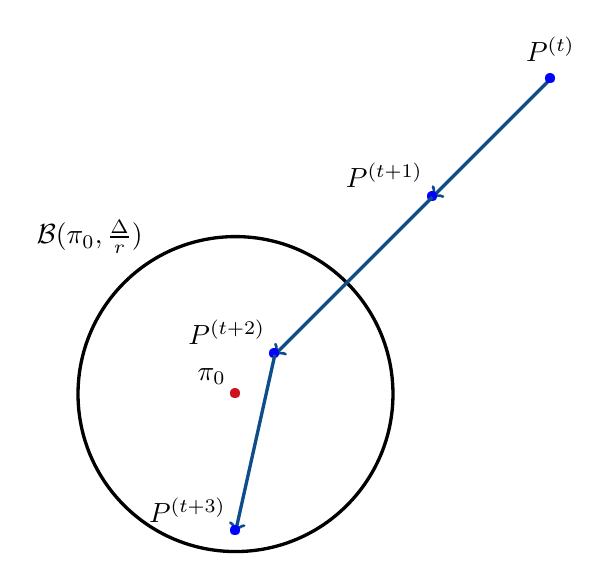
\begin{tikzpicture}
  \draw[very thick] (0,0) circle (2cm);
  \coordinate (A) at (4,4);
  \coordinate (B) at (2.5,2.5);
  \coordinate (C) at (0,0);
  \coordinate (D) at (0.5,0.5);
  \coordinate (E) at (0,-1.75);


   \draw [->, very thick, dodgerblue] (A)--(B);
  \node [blue] at (A) {\textbullet};
  \node at (A) [above = 1mm of A] {$P^{(t)}$};
  \node [blue] at (B) {\textbullet};
  \node at (B) [above left] {$P^{(t+1)}$};
  \draw [->, very thick, dodgerblue] (B)--(D);
  \node [blue] at (D) {\textbullet};
  \node at (D) [above left] {$P^{(t+2)}$};
  \draw [->, very thick, dodgerblue] (D)--(E);
  \node [blue] at (E) {\textbullet};
  \node at (E) [above left] {$P^{(t+3)}$};
  \node [red3] at (C) {\textbullet};
  \node at (C) [above left] {$\pi_0$};
  \node at (-1.85,2) {$\mathcal{B}(\pi_0,\frac\Delta r)$};
    \end{tikzpicture}
\end{figure}

\begin{theorem}
\label{th:1}
Making the same assumptions as in Lemma \ref{korattikara_lemma}, the total variation distance between $\pi_0$ and $\pi_\varepsilon$ is upper bounded as follows : $$d_T(\pi_0,\pi_\varepsilon)\leq\frac{\Delta_{max}}{1-\eta}$$
where $\Delta_{max}\equiv\sup_{\theta,\theta'}|\alpha_\varepsilon(\theta,\theta')-\alpha_0(\theta,\theta')|$ and $\eta\in[0,1)$
\end{theorem}
In the proof provided by \cite{korattikara2014austerity}, we have spotted a mistake in the definition of the Metropolis-Hastings transition kernel which in turn leads to a flawed proof. They indeed write this kernel as 
\begin{align*}
    &\mathcal K_0(\theta,\theta')=\alpha_0(\theta,\theta')q(\theta'|\theta)+\delta_\theta(\theta')(1-\alpha_0(\theta,\theta'))
    \intertext{Instead of}
    &\mathcal K_0(\theta,\theta')=\alpha_0(\theta,\theta')q(\theta'|\theta)+\delta_\theta(\theta')(1-r_0(\theta))
    \intertext{where}
    &r_0(\theta)=\int_{\theta'}\alpha_0(\theta,\theta')q(\theta'|\theta)d\theta'
\end{align*} 
as can be seen on Figure \ref{fig:korattikara_appendix} in Appendix where we provide a screenshot of the proof given in the article. This is not simply a typo, as later in the proof it is clear they use $\alpha_0$ instead or $r_0$.\\
However, the corrected proof we provide below does lead to the same result.\\
\textit{Proof.} Now that Lemma (\ref{korattikara_lemma}) is proved, there only remains to show that for any probability measure $P$, 
\begin{align}
\label{eq:korattikara9}
d_T(P\mathcal{K}_0,P\mathcal{K}_\varepsilon)=\frac12\int_{\theta'\in\Theta}|(P\mathcal{K}_\varepsilon)(\theta')-(P\mathcal{K}_0)(\theta')|d\theta'\leq\Delta_{max}
\end{align}
where $\Delta_{max}:=\sup_{\theta,\theta'}|\alpha_\varepsilon(\theta,\theta')-\alpha_0(\theta,\theta')|$.\\

In the ApMHT algorithm, the transition kernel $\mathcal{K}_\varepsilon$ is
$$\mathcal{K}_\varepsilon(\theta,\theta')=\alpha_\varepsilon(\theta,\theta')q(\theta'|\theta)+\delta_\theta(\theta')(1-r_\varepsilon(\theta))$$
where we use the approximate acceptance probability $\alpha_\varepsilon$ instead of $\alpha_0$ and $r_\varepsilon$ is defined in a similar way as $r_0$.\\ 
Let $\Delta_\alpha:=\alpha_\varepsilon-\alpha_0$ the error in the acceptance probability. Clearly, this quantity is upper-bounded by $\Delta_{max}$ as $|\Delta_\alpha|\leq\Delta_{max}$, by definition of $\Delta_{max}$.\\
\textit{Proof of} (\ref{eq:korattikara9}). For all $P$ probability measure,
\begin{align*}
&\frac12\int_{\theta'\in\Theta}|(P\mathcal{K}_\varepsilon)(\theta')-(P\mathcal{K}_0)(\theta')|d\theta'\\
=&\frac12\int_{\theta'\in\Theta}\left|\int_{\theta\in\Theta}(P\mathcal{K}_\varepsilon)(\theta,\theta')-(P\mathcal{K}_0)(\theta,\theta')dP(\theta)\right|d\theta'\\
=&\frac12\int_{\theta'\in\Theta}\left|\int_{\theta\in\Theta}(\alpha_\varepsilon(\theta,\theta')q(\theta'|\theta)+\delta_\theta(\theta')(1-r_\varepsilon(\theta))-\alpha_0(\theta,\theta')q(\theta'|\theta)-\delta_\theta(\theta')(1-r_0(\theta)))dP(\theta)\right|d\theta'\\
=&\frac12\int_{\theta'\in\Theta}\left|\int_{\theta\in\Theta}q(\theta'|\theta)\Delta_\alpha(\theta,\theta')-\delta_\theta(\theta')(r_\varepsilon(\theta)-r_0(\theta))dP(\theta)\right|d\theta'\\
\le&\frac12\int_{\theta'\in\Theta}\int_{\theta\in\Theta}q(\theta'|\theta)|\Delta_\alpha(\theta,\theta')|+\delta_\theta(\theta')|r_\varepsilon(\theta)-r_0(\theta)|dP(\theta) d\theta'\\
\end{align*}
Where
\begin{align*}
|r_\varepsilon(\theta)-r_0(\theta)|&=\left |\int_{\theta'}(\alpha_\varepsilon(\theta,\theta')-\alpha_0(\theta,\theta'))q(\theta'|\theta)d\theta'\right |\\
&\le\int_{\theta'}|\alpha_\varepsilon(\theta,\theta')-\alpha_0(\theta,\theta')|q(\theta'|\theta)d\theta'\\
&\le \Delta_{max}\int_{\theta'}q(\theta'|\theta)d\theta'\\
&=\Delta_{max}
\end{align*}
Hence
\begin{align*}
&\frac12\int_{\theta'\in\Theta}|(P\mathcal{K}_\varepsilon)(\theta')-(P\mathcal{K}_0)(\theta')|d\theta'\\
\le&\frac12 \Delta_{max}\int_{\theta'\in\Theta}\int_{\theta\in\Theta}q(\theta'|\theta)+\delta_\theta(\theta')dP(\theta) d\theta'\\
=&\Delta_{max}
\end{align*}\qed\\
One might be worried that $\Delta_{max}$ is large. However recall that if $\varepsilon\rightarrow0$, then the batch size $m$ tends to $N$ which in turn implies that $\alpha_\varepsilon\rightarrow\alpha_0$. Hence, provided we choose $\varepsilon$ small enough, the upper-bound derived in Theorem \ref{th:1} is guaranteed to be small. Under this condition, ApMHT should yield a good approximation of the posterior $\pi_0$.
\newpage
\section{Stochastic Gradient Langevin Dynamics (SGLD)}
\label{sec:SGLD_exp}
We now present the second of the algorithms we consider.
\par Stochastic Gradient Langevin Dynamics (SGLD, \cite{welling2011bayesian}) has two major assets when applied to Bayesian posterior sampling in the context of Big Data. Firstly, it only requires a fraction of size $m\ll N$ of the total data set at each iteration. Secondly, it can be tuned to become a rejection-free algorithm, ensuring that every candidate $\theta'$ is accepted at each step, which once again reduces the total computational cost as we bypass the evaluation of the acceptance probability $\alpha$ of standard Metropolis-Hastings (MH, \cite{metropolis1953equation}).\\
This class of algorithms combines two major concepts, namely Langevin Monte Carlo theory (LMC, \cite{roberts1998optimal}) and stochastic gradient which we review below.\\
LMC relies on the overdamped Langevin \^Ito diffusion, or Langevin equation.
\begin{equation}
\label{eq:langevin}
d\theta_t=\frac 12\nabla_{\theta_t} \log\pi(\theta_t|z)+d\eta_t
\end{equation}
where $\eta_t$ is a d-dimensional Wiener Process.\\
However, the use of digital computers requires a discretised version of (\ref{eq:langevin}). Equation (\ref{eq:langevin_discr}) can then be used as a proposal distribution in standard MH.
\begin{equation}
\label{eq:langevin_discr}
\theta_{t+1}=\theta_t+\frac \varepsilon 2\nabla_{\theta_t} \log\pi(\theta_t|z)+\eta_t
\end{equation}
where $\eta_t\sim\mathcal N(0,\varepsilon_t)$. \\
This discretisation process comes at the expense of the rejection-free property of exact LMC. Indeed, an expensive MH accept-reject step is essential to correct the discretisation error in order to target the true posterior. However, as $\varepsilon\rightarrow0$, the discretisation error decreases so that the acceptance probability $\alpha$\ tends back to $1$, making the accept-reject step unnecessary, if an approximate target is acceptable.\\
SGLD is, in its original form, an asymptotically exact algorithm which builds upon the latter and introduces the use of mini-batches of data in order to further enhance computational efficiency when evaluating the gradient of the posterior.
In fact, the update step of SGLD goes as follows.\\
Let $\mathcal I\subset \{1,...,N\}$ be an index subset of size $m\ll N$,

\begin{equation}
\label{eq:SGLD}
\theta_{t+1}=\theta_t+\frac{\varepsilon_t}{2}\underbrace{\left(\nabla_{\theta_t} \log\pi(\theta_t)+\frac{N}{n}
\sum_{i\in\mathcal I}\nabla_{\theta_t}\log p(z_i|\theta_t)\right)}_{\text{stochastic gradient}}+\underbrace{\eta_t}_{\text{injected noise}}
\end{equation}
where $\eta_t\sim\mathcal N(0,\varepsilon_t)$ and

\begin{align}
\label{eq:SGLD_cond}
\sum_{t=1}^\infty \varepsilon_t=\infty \quad\text{and}\quad \sum_{t=1}^\infty \varepsilon_t^2<\infty
\end{align}

In (\ref{eq:SGLD_cond}), the first condition ensures good mixing of the Markov chain whereas the second makes sure that the chain does converge to the model.\\
\cite{welling2011bayesian} give an informal intuition as to why SGLD produces samples that asymptotically approach the true posterior $\pi(\theta|z)$, i.e why (\ref{eq:SGLD}) is equivalent to (\ref{eq:langevin_discr}) as $t\rightarrow\infty$. \\
Stochasticity comes from two factors in (\ref{eq:SGLD}), namely the stochastic gradient and the injected Gaussian noise $\eta_t$. It is easy to see that they respectively have a variance of $O(\varepsilon^2_t)$ and $O(\varepsilon_t)$. Hence, as $t\rightarrow\infty$, (\ref{eq:SGLD_cond}) implies that $\varepsilon_t\rightarrow 0$, which in turn implies that the injected noise dominates the stochastic gradient noise. Therefore, one should expect SGLD to sample from the true posterior approximately as $t\rightarrow\infty$. Besides, since $\varepsilon_t\rightarrow 0$, the acceptance probability $\alpha$ tends to 1 which makes the accept-reject step unnecessary. \\
However, in practice, it is common to use a small constant step-size $0<\varepsilon\ll 1$ tuned in order to be big enough to guarantee good mixing and small enough to bypass the MH accept-reject step. The algorithm is then no longer asymptotically exact.\\
Below is given a possible implementation of the algorithm.\\
\\
\begin{algorithm}[H]
\label{algo:SGLD}
\setstretch{1}
 \SetKwInOut{Input}{Input}
 \SetKwInOut{Output}{Output}
 \Input{data $z$, $\varepsilon$, $T$, $m$, $\theta_0$}
 \Output{$\theta=\{\theta_t\}_{t=0}^T$ approximately drawn from $\pi(\theta|z)\propto p(z|\theta)\pi(\theta)$}
 Initialization\;
 \For{$t=0,...,T$}{
 Draw minibatch of size m $\mathcal X\subset z$ without replacement\;
 Draw $\eta\sim\mathcal N(0,\varepsilon^2)$\;
 $\theta_{t+1}=\theta_t+\frac{\varepsilon}{2}\left(\nabla_{\theta_t}\log\pi(\theta_t)+\frac Nm\nabla_{\theta_t} \log p(\mathcal X|\theta_t)+\eta\right)$\;
 }
 \caption{'Approximate' SGLD}
\end{algorithm}

\newpage
\section{Consensus Monte-Carlo}
\label{sec:consensus_exp}
We now present the third algorithm reviewed in this study.\\
Parallelising MCMC computations is another strategy that can be implemented in order to bypass large likelihood evaluations. This class of methods splits the data into smaller batches and distribute them to several cores or machines. 
Assume, $M$ machines are available. Making the assumption that the observations are conditionally independent given $\theta$, the posterior distribution can be written as follows :
  \begin{equation}
\label{eq:consensus1}
\pi(\theta|z)\propto\prod_{m=1}^M\pi(\theta)^{1/M}p(\textbf{z}_m|\theta)
\end{equation}
where $\{\textbf{z}_1, ..., \textbf{z}_M\}$ denote subsets of data set $z$ and $\forall 1\le i,j\le M$, $\textbf{z}_i\cap\textbf{z}_j=\emptyset$.
  Then, the user can run independently and simultaneously standard MCMC methods on batches of size $m\ll N$ if $M$ is large enough, which should decrease the total computation time dramatically. Note that machine $m\in\{1,...,M\}$ will generate samples $\{\theta_t^m\}_t$ from an algorithm targeting $\pi_m(\theta|z)\propto\pi(\theta)^{1/M}p(\textbf{z}_m|\theta)$. This first step is a common feature of most algorithms using this so-called \textit{divide-and-conquer} strategy (\cite{bardenet2017markov}). They differ however on how to combine the $M$ generated samples in order to obtain samples $\{\theta_t\}_t \sim \pi(\theta|z)$, i.e distributed according to the true posterior.\\
  
  \begin{figure}[H]
    \centering
    \caption{Parallel MCMC strategy}
    \label{fig:consensus1}

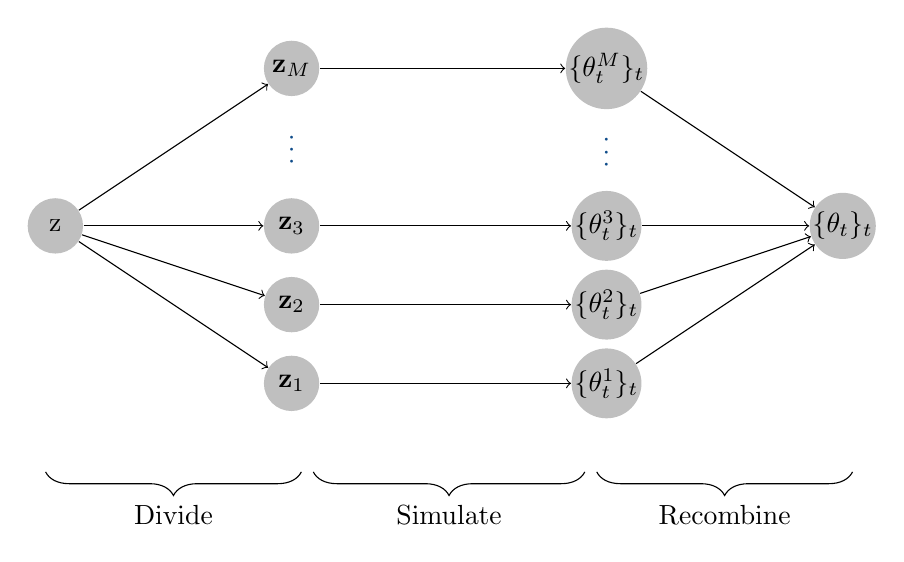
\begin{tikzpicture}
  \node[vertex] (n1)  at (0,4)  {z};
  \node[vertex] (n2)  at (3,2)  {$\textbf{z}_1$};
  \node[vertex] (n3)  at (3,3)  {$\textbf{z}_2$};
  \node[vertex] (n4)  at (3,4)  {$\textbf{z}_3$};
  \node[vertex] (n5)  at (3,6)  {$\textbf{z}_M$};
  \node[vertex] (n6)  at (10,4) {$\{\theta_t\}_t$};
  \node[vertex] (n7)  at (7,6)  {$\{\theta_t^M\}_t$};
  \node[vertex] (n8)  at (7,4)  {$\{\theta_t^3\}_t$};
  \node[vertex] (n9)  at (7,3)  {$\{\theta_t^2\}_t$};
  \node[vertex] (n10) at (7,2)  {$\{\theta_t^1\}_t$};
  \node (n11) at (0,1)  {};
  \node (n12) at (3,1)  {};
  \node (n13) at (3.4,1)  {};
  \node (n14) at (6.6,1)  {};
  \node (n15) at (7,1)  {};
  \node (n16) at (10,1)  {};
  
  \path (n4) -- (n5) node [dodgerblue, midway, sloped] {$\dots$};
  \path (n8) -- (n7) node [dodgerblue, midway, sloped] {$\dots$};

  \foreach \from/\to in {n1/n2,n1/n3,n1/n4,n1/n5,
                n7/n6,n8/n6,n9/n6,n10/n6,n5/n7,n4/n8,n3/n9,n2/n10}
      \draw[->] (\from) -- (\to);
      
\draw[decorate,decoration={brace,amplitude=3mm,mirror}](n11.south west)--(n12.south east)node [midway,yshift=-0.55cm] {Divide};
\draw[decorate,decoration={brace,amplitude=3mm,mirror}](n13.south west)--(n14.south east)node [midway,yshift=-0.55cm] {Simulate};
\draw[decorate,decoration={brace,amplitude=3mm,mirror}](n15.south west)--(n16.south east)node [midway,yshift=-0.55cm] {Recombine};
 \end{tikzpicture}
\end{figure}

\cite{scott2016bayes} suggest using the \textit{Consensus Monte-Carlo} algorithm. This method uses intensively the Bernstein-Von Mises theorem and its extension by \cite{le2012asymptotics} which states that under some regularity conditions, the posterior distribution is asymptotically independent from the prior and follows a normal distribution concentrated around the true value of the estimated parameter with variance equal to the inverse of the Fischer information matrix. In particular, one can make the assumption that $\theta|\textbf{z}_m$, $m=1,...,M$ is normally distributed, provided that $|\textbf{z}_m|$ is large enough.\\
We prove the following lemma \ref{lemma_consensus} and property \ref{eq:consensus3} which are at the core of \cite{scott2016bayes}'s algorithm and are left unproved in their article as a bit too obvious.
\begin{lemma}
\label{lemma_consensus}
Suppose that $M=2$. This can be assumed without loss of generality as the following method may be iterated. If
\begin{align*}
\theta|\textbf{z}_1\sim\mathcal{N}(\mu_1,\Sigma_1)\nonumber
\quad\text{and}\quad
\theta|\textbf{z}_2\sim\mathcal{N}(\mu_2,\Sigma_2)\nonumber
\end{align*}
then
\begin{equation}
\label{eq:consensus2}
\theta|z\sim\mathcal N(\mu,\Sigma)
\end{equation}
where
\begin{align*}
\Sigma=(\Sigma_1^{-1}+\Sigma_2^{-1})^{-1}\quad \text{and}\quad \mu=\Sigma(\Sigma_1^{-1}\mu_1+\Sigma_2^{-1}\mu_2)
\end{align*}
\end{lemma}
\textit{Proof.}\begin{align*}
\pi(\theta|z)&\propto\pi(\theta|\textbf{z}_1)\pi(\theta|\textbf{z}_2)\\
&\propto \exp\left(-\frac12\left[(\theta-\mu_1)^T\Sigma_1^{-1}(\theta-\mu_1)+(\theta-\mu_2)^T\Sigma_2^{-1}(\theta-\mu_2)\right]\right)\\
&\propto \exp\left(-\frac12\left[\theta^T(\Sigma_1^{-1}+\Sigma_2^{-1})\theta -2(\Sigma_1^{-1}\mu_1+\Sigma_2^{-1}\mu_2)^T\theta\right]\right)\text{ by symmetry of } \Sigma_1\text{ and } \Sigma_2\\
&\propto \exp\left(-\frac12\left[(\theta-\Sigma(\Sigma_1^{-1}\mu_1+\Sigma_2^{-1}\mu_2))\Sigma^{-1}(\theta-\Sigma(\Sigma_1^{-1}\mu_1+\Sigma_2^{-1}\mu_2))^T\right]\right)\text{ by completing the square}\\
&\propto \exp\left(-\frac12\left[(\theta-\mu))\Sigma^{-1}(\theta-\mu))^T\right]\right) 
\end{align*}\qed
\begin{property}
\label{eq:consensus3}
Let $\theta_1\sim\mathcal N(\mu_1,\Sigma_1)$ and $\theta_2\sim\mathcal N(\mu_2,\Sigma_2)$.\\
Then $\Sigma(\Sigma_1^{-1}\theta_1+\Sigma_2^{-1}\theta_2)\sim\mathcal N(\mu,\Sigma)$
  \end{property} 
\textit{Proof.} It is clear that the quantity of interest is normal, as a linear combination of normally-distributed variables. Now
\begin{itemize}

\item $\mathbb E[\Sigma(\Sigma_1^{-1}\theta_1+\Sigma_2^{-1}\theta_2)]=\Sigma(\Sigma_1^{-1}\mu_1+\Sigma_2^{-1}\mu_2)=\mu$
  \item $\mathbb{V}\left(\Sigma(\Sigma_1^{-1}\theta_1+\Sigma_2^{-1}\theta_2)\right)=\mathbb{V}\left(\Sigma\Sigma_1^{-1}\theta_1\right)+\mathbb{V}\left(\Sigma\Sigma_2^{-1}\theta_2\right)=\Sigma(\Sigma_1^{-1}+\Sigma_2^{-1})\Sigma=\Sigma\qed$
  \end{itemize}

Hence, assuming the posterior is asymptotically normal, as is the case if Bernstein-Von Mises theorem applies, and the number of data points is large, then by Lemma \ref{lemma_consensus} and Property \ref{eq:consensus3}, \cite{scott2016bayes} combine the obtained $M$ samples by applying the following formula in order to target the full posterior : \\
Suppose machine $m$ generates sample $\theta_{m1},...,\theta_{mT}$. Then $\forall t\in\{1,...,T\}$,
\begin{align}
\label{eq:consensus4}
\theta_t=\left(\sum_{m=1}^M\Sigma_m^{-1}\right)^{-1}\sum_{m=1}^M\Sigma_m^{-1}\theta_{mt}
\end{align}
Note that this is simply a weighted average of the subposterior samples with weights $\Sigma_m^{-1}$, $m=1,...,M$. In practice, only an estimate of the weights can be computed as seen in the algorithm below.

\begin{algorithm}[H]
\label{algo:2}
\setstretch{1}
\SetKwInOut{Input}{Input}
\SetKwInOut{Output}{Output}
\Input{samples $\theta_m=\{\theta_{mt}\}_{t=1}^T$ each from $\pi(\theta|z_s)\propto p(\textbf{z}_m|\theta)\pi(\theta)^{1/M}$ where $\textbf{z}_m$ denotes subsets of the data for $m=1,...,M$}
\Output{$\theta=\{\theta_t\}_{t=0}^T$ asymptotically from $\pi(\theta|z)\propto p(z|\theta)\pi(\theta)$}
Initialization\;
$W_m\leftarrow \left(var(\{\theta_{mt}\}_{t=1}^T)\right)^{-1}$ for $m=1,...,M$\;
$W\leftarrow \sum_{m=1}^M W_m$\;
$\theta\leftarrow 0$\;
\For{$m=1,...,M$}{
  $\theta=\theta+W_m\theta_m$\;
}
$\theta=W^{-1}\theta$
  \caption{Consensus Monte Carlo}
\end{algorithm}
One can notice that if the posterior distribution is normal, then this algorithm targets exactly the posterior. However if the posterior is only assymptotically normal by the Bernstein-Von Mises theorem, then Consensus Monte-Carlo is only asymptotically exact.
\newpage
\section{Asymptotically exact sampling via non-parametric density product estimation}
\label{sec:neiswanger_exp}
We now introduce the fourth algorithm of our study.\\
The \textit{Non-Parametric Density Product Estimator} (NPDPE) algorithm described by \cite{neiswanger2013asymptotically} comes as a more flexible alternative to the \textit{Consensus Monte-Carlo} described in Section \ref{sec:consensus_exp}. With \textit{Consensus Monte-Carlo} one could expect substantial issues in cases where the Bernstein-Von Mises theorem does not hold. NPDPE however does not make such assumptions on the asymptotic behaviour of the posterior distribution.\\
As in Section \ref{sec:consensus_exp}, we rewrite the posterior distribution as

\begin{equation}
\label{eq:neiswanger1}
\pi(\theta|z)\propto\prod_{m=1}^M\pi(\theta)^{1/M}p(\textbf{z}_m|\theta)
\end{equation}
where $\{\textbf{z}_1, ..., \textbf{z}_M\}$ denote subsets of data set $z$ and $\forall 1\le i,j\le M$, $\textbf{z}_i\cap\textbf{z}_j=\emptyset$.
Assuming we have obtained thanks to standard MCMC methods $T$ samples $\{\theta_{t_m}^m\}_{t_m=1}^T$ for each subposterior $\pi_m$, \cite{neiswanger2013asymptotically} propose the following kernel estimator $\hat \pi_m$

\begin{equation}
\label{eq:neiswanger2}
    \hat \pi_m(\theta)=\frac1T\sum_{t_m=1}^T\frac{1}{h^d}\mathcal{K}\left(\frac{||\theta-\theta_{t_m}^m||}{h}\right)
\end{equation}
where $\mathcal K$ denotes any kernel function with bandwidth $h\in\mathbb R^{+}$. We will use from now on a standard Gaussian kernel, i.e 

\begin{equation}
\label{eq:neiswanger3}
    \hat \pi_m(\theta)=\frac1T\sum_{t_m=1}^T\mathcal{N}_d(\theta|\theta_{t_m}^m,h^2 I_d)
\end{equation}
Now, the estimator of the posterior distribution suggested by \cite{neiswanger2013asymptotically} is simply the product of the subposterior estimators defined in (\ref{eq:neiswanger3}), hence the name \textit{Non-Parametric Density Product Estimator} :

\begin{align}
    \label{eq:neiswanger4}
    \widehat{\pi_1...\pi_M}(\theta)&=\hat\pi_1(\theta)...\hat\pi_M(\theta)\nonumber\\
    &=\frac{1}{T^M}\prod_{m=1}^M\sum_{t_m=1}^T \mathcal{N}_d(\theta|\theta_{t_m}^m,h^2 I_d)\nonumber\\
    &\propto\sum_{t_1=1}^T...\sum_{t_M=1}^T\underbrace{\left[\prod_{m=1}^M\mathcal N_d\left(\theta_{t_m}^m\bigg|\frac1M\sum_{m=1}^M\theta_{t_m}^m,h^2I_d\right)\right]}_\text{weight}
    \mathcal N_d\left(\theta\bigg|\frac1M\sum_{m=1}^M\theta_{t_m}^m,\frac{h^2}{M}I_d\right)
\end{align}
which can be derived through a straightforward but tedious computation.\\
Although (\ref{eq:neiswanger4}) is a large mixture of $T^M$ normal distributions, one can  sample rather easily from it. One should first sample a mixture weight by using a Metropolis within Gibbs sampler and then sampling from the normal distribution associated with the sampled weight. A complete description of this procedure is given in Algorithm \ref{algo:neiswanger}.\\
In practice, we find that tuning the bandwidth $h$ to a constant small number yields more efficient mixing. Also, in order to prevent computational stability issues, we find that the accept-reject step performed in line \texttt{23} is much more reliable when the ratio of weights is log-transformed. Hence, we recommend that line \texttt{23} be written as follows : 
$$\textbf{\texttt{if}} \log(u)<\log(w_c)-log(w_{\tilde{t}}) \textbf{\texttt{ then}}$$

\begin{algorithm}[H]
\label{algo:neiswanger}
\setstretch{1}
\SetKwInOut{Input}{Input}
\SetKwInOut{Output}{Output}
\Input{samples $\theta_m=\{\theta_{mt}\}_{t=1}^T$ each from $\pi(\theta|z_s)\propto p(\textbf{z}_m|\theta)\pi(\theta)^{1/M}$ where $\textbf{z}_m$ denotes subsets of the data for $m=1,...,M$}
\Output{$\theta=\{\theta_t\}_{t=0}^T$ asymptotically from $\pi(\theta|z)\propto p(z|\theta)\pi(\theta)$}
Initialization\;
$\tilde t=\{t_1,...,t_M\}\overset{i.i.d}{\sim}\mathcal{U}_{\{1,...,T\}}$\;
\For{$i=1,...,T$}{
  $h\leftarrow i^{-1/(4+d)}$\;
  \For{$m=1,..,M$}{
    $c\leftarrow \tilde t$\;
    $c_m\sim\mathcal U_{\{1,...,T\}}$\;
    $\bar\theta_{\tilde t}\leftarrow 0$\;
    $\bar\theta_c\leftarrow 0$\;
    $w_{\tilde t}\leftarrow 1$\;
    $w_c\leftarrow 1$\;
    \For{$j=1,...,m$}{
        $\bar\theta_{\tilde t}\leftarrow\bar\theta_{\tilde t}+\theta_{\tilde t_j}^j$\;
        $\bar\theta_c\leftarrow\bar\theta_c+\theta_{c_j}^c$\;
    }
    $\bar\theta_{ \tilde t}\leftarrow\frac1M \bar\theta_{ \tilde t}$\;
    $\bar\theta_c\leftarrow\frac1M \bar\theta_c$\;
    \For{$j=1,...,m$}{
        $w_{\tilde t}\leftarrow w_t\times\mathcal N(\theta_{\tilde t_j}^j|\bar\theta_{\tilde t},h^2 I_d)$\;
        $w_c\leftarrow w_c\times\mathcal N(\theta_{c_j}^j|\bar\theta_c,h^2 I_d)$\;
    }
    $u\sim\mathcal U_{[0,1]}$\;
    \If{$u<w_c/w_{\tilde t}$}{
        $\tilde t\leftarrow c$\;
        $\bar\theta_{\tilde t}\leftarrow\bar\theta_{c}$
    }
  }
  $\theta_i\sim\mathcal N_d(\bar\theta_{\tilde t},\frac{h^2}{M}I_d)$
    
}
$\theta=W^{-1}\theta$
  \caption{NPDPE}
\end{algorithm}

It can be shown that the density product estimator $\widehat{\pi_1...\pi_M}$ of $\pi_1...\pi_M$ is consistent in Mean Squared error i.e that $MSE(\widehat{\pi_1...\pi_M})\longrightarrow0$ as $T\longrightarrow\infty$.
Define the H\"older class $\Sigma (\beta,C)$, for $\beta\geq1$ and $C>0$ to be the set of functions $f : \mathcal X\longmapsto\mathbb R$ $l$-times differentiable for $l=\lfloor\beta\rfloor$ such that
$$|f^{(l)}(\theta)-f^{(l)}(\theta')|\leq C||\theta-\theta'||^{\beta-l},\quad \forall \theta,\theta'\in\mathcal X$$
Let $\mathcal P(\beta,C)=\left\{p\in\Sigma(\beta,C)|p\geq0,\;\int p(\theta)d\theta=1\right\}$\\
Assume that for all $1\leq m\leq M$, subposterior $\pi_m\in\mathcal{P}(\beta,C)$ and $\exists b>0$ s.t $\pi_m(\theta)\leq b$, $\forall\theta\in\mathcal X$.
\cite{neiswanger2013asymptotically} first derive an upper bound for the bias of their estimator $\widehat{\pi_1...\pi_M}$ of $\pi_1...\pi_M$.\\

\noindent The authors state and prove the following lemma. Our contribution is the explicit derivation of the upper-bound for $|\mathbb{E}[\hat \pi_m(\theta)]-\pi_m(\theta)|$.
\begin{lemma}
\label{neiswanger_lemma1}
$$\sup\limits_{\pi_1,...,\pi_M\in\mathcal P(\beta,C)}|\mathbb E[\widehat{\pi_1...\pi_M}(\theta)]-\pi_1...\pi_M(\theta)|\leq\sum_{m=1}^M c_mh^{m\beta}$$ for some $c_1,...,c_M>0$
\end{lemma}
\noindent\textit{Proof.} Let $\pi_1,...,\pi_m\in\mathcal P(\beta,C)$,
\begin{align*}
|\mathbb E[\widehat{\pi_1...\pi_M}(\theta)]-\pi_1...\pi_M(\theta)|&=|\mathbb E[\hat \pi_1(\theta)...\hat \pi_M(\theta)]-\pi_1...\pi_M(\theta)|\\
&=|\mathbb E[\hat \pi_1(\theta)]...\mathbb E[\hat \pi_M(\theta)]-\pi_1...\pi_M(\theta)|
\intertext{Now,}
|\mathbb{E}[\hat \pi_m(\theta)]-\pi_m(\theta)|&=\left|\frac1T\sum_{t_m=1}^T\int\mathcal N(\theta|\theta_{t_m}^m,h^2I_d)\pi_m(\theta_{t_m}^m)d\theta_{t_m}^m-\pi_m(\theta)\right|\\
&=\left|\frac1T\sum_{t_m=1}^T\int\mathcal N(\theta|\theta_{t_m}^m,h^2I_d)(\pi_m(\theta_{t_m}^m)-\pi_m(\theta))d\theta_{t_m}^m\right|\\
&=c\left|\sum_{t_m=1}^T\int\exp\left\{\frac12\left(\frac{||\theta_{t_m}^m-\theta||}{h}\right)^2\right\}(\pi_m(\theta_{t_m}^m)-\pi_m(\theta))d\theta_{t_m}^m\right|, \text{ $c> 0$}
\intertext{Let $y_m=\frac{\theta_{t_m}^m-\theta}{h}$. Then,}
|\mathbb{E}[\hat \pi_m(\theta)]-\pi_m(\theta)|&=\tilde{c}\left|\sum_{m=1}^T\int\exp\left\{\frac12||y_m||^2\right\}(\pi_m(\theta+hy_m)-\pi_m(\theta))dy_m\right|, \text{ $\tilde c> 0$}\\
&\leq\tilde{c}\sum_{m=1}^T\int\exp\left\{\frac12||y_m||^2\right\}\left|\pi_m(\theta+hy_m)-\pi_m(\theta)\right|dy_m\\
&\leq\tilde{c}Ch^\beta\sum_{m=1}^T\int\exp\left\{\frac12||y_m||^2\right\}|y_m|dy_m, \text{ since $\pi_m\in\mathcal P(\beta,C)$}\\
&\leq c_m'h^\beta, \text{ $c_m'> 0$, since the moments of a Gaussian are bounded.}
\intertext{Hence,}
|\mathbb E[\widehat{\pi_1...\pi_M}(\theta)]-\pi_1...\pi_M(\theta)|&=|\mathbb E[\hat \pi_1(\theta)]...\mathbb E[\hat \pi_M(\theta)]-\pi_1...\pi_M(\theta)|\\
&\leq |(\pi_1(\theta)+c_1'h^{\beta})...(\pi_M(\theta)+c_M'h^{\beta})-\pi_1...\pi_M(\theta)|\\
&\leq |c_1h^{\beta}+...+c_Mh^{M\beta}|\text{ where $c_1,...,c_M$>0}\\
&\leq |c_1h^{\beta}|+...+|c_Mh^{M\beta}|\\
&=\sum_{m=1}^Mc_m h^{m\beta}
\end{align*}\qed

The authors then derive an upper bound for the variance of their density product estimator. Our contribution to this proof is the explicit derivation of an upper-bound for $\mathbb{V}[\hat \pi_m(\theta)]$, $\forall \; 1\le m\le M$.

\begin{lemma}
\label{neiswanger_lemma2}
$$\sup\limits_{\pi_1,...,\pi_M\in\mathcal P(\beta,C)}\mathbb V[\widehat{\pi_1...\pi_M}(\theta)]\leq\sum_{m=1}^M \binom Mm\frac{c_m}{T^m}{h^{dm}}$$ for some $c_1,...,c_M>0$
\end{lemma}
\noindent\textit{Proof.} Let us first derive an upper-bound for $\mathbb{V}[\hat \pi_m(\theta)]$, $\theta\in\mathcal X$, $1\leq m\leq M$.

\begin{align*}
\mathbb{V}[\hat \pi_m(\theta)]&\leq\mathbb{E}[\hat \pi_m(\theta)^2]=c\frac{1}{Th^{2d}}\sum_{t_m=1}^T\int\exp\left\{\left(\frac{||\theta_{t_m}^m-\theta||}{h}\right)^2\right\}\pi_m(\theta_{t_m}^m)d\theta_{t_m}^m, \text{ $c> 0$}
\intertext{Let $y_m=\frac{\theta_{t_m}^m-\theta}{h}$. Then,}
\mathbb{V}[\hat \pi_m(\theta)]&=c\frac{h^d}{Th^{2d}}\sum_{m=1}^T\int\exp\left\{||y_m||^2\right\}\pi_m(hy_m+\theta)dy_m\\
&\leq c\frac{\sup_{\theta}\pi_m(\theta)}{Th^d}\sum_{m=1}^T\int\exp\left\{||y_m||^2\right\}dy_m\\
&\leq \frac{c'_m}{Th^d}
\intertext{Now, }
\mathbb V[\widehat{\pi_1...\pi_m}(\theta)]&=\mathbb{E}[\hat \pi_1(\theta)^2]...\mathbb{E}[\hat \pi_M(\theta)^2]-\mathbb{E}[\hat \pi_1(\theta)]^2...\mathbb{E}[\hat \pi_M(\theta)]^2\\
&=\left(\prod_{m=1}^M\mathbb{V}[\hat \pi_m]+\mathbb E[\hat \pi_m]^2\right)-\left(\prod_{m=1}^M\mathbb E[\hat \pi_m]^2\right)\\
&\leq\sum_{m=0}^{M}\binom{M}{m}\frac{\tilde{c}^mc^{M-m}}{T^{M-m}h^{d(M-m)}}-\tilde c^M 
\intertext{where $\tilde c=\max\{c_1,...,c_M\}$, $\{c_1,...,c_M\}$ being the upper-bounds derived in lemma \ref{neiswanger_lemma1} and $c=\max\{c'_1,...,c'_M\}$ }
&=\sum_{m=0}^{M-1}\binom{M}{m}\frac{\tilde{c}^mc^{M-m}}{T^{M-m}h^{d(M-m)}}\\
&\leq\sum_{m=1}^{M}\binom{M}{m}\frac{c_m}{T^{m}h^{dm}}, \text{where $c_m>0$ $\forall m$}
\end{align*}\qed

\cite{neiswanger2013asymptotically} then use results from lemma \ref{neiswanger_lemma1} and \ref{neiswanger_lemma2} to derive an upper bound on the Mean-Squared Error (MSE)

\begin{proposition}
If $h\asymp T^{-1/(2\beta+d)}$ then 
\begin{align}
\label{eq:neiswanger6}
\sup\limits_{\pi_1,...,\pi_M\in\mathcal P(\beta,C)}\text{MSE}(\widehat{\pi_1...\pi_M}(\theta))&=\sup\limits_{\pi_1,...,\pi_M\in\mathcal P(\beta,C)}\mathbb E \left [\int (\widehat{\pi_1...\pi_M}(\theta)-\pi_1...\pi_M(\theta))^2d\theta\right]\nonumber\\
&\leq \frac{c}{T^{2\beta/(2\beta+d)}}
\end{align}
for $c>0$ and $0< h\leq 1$
\end{proposition}


\noindent \textit{Proof.}
For $\pi_1,...,\pi_M\in\mathcal P(\beta,C)$, using the bias-variance decomposition of the MSE,
\begin{align*}
\mathbb E \left [\int (\widehat{\pi_1...\pi_M}(\theta)-\pi_1...\pi_M(\theta))^2d\theta\right]&\leq\left(\sum_{m=1}^M c_mh^{mb}\right)^2+\sum_{m=1}^M \binom Mm \frac{\tilde c_m}{T^mh^{dm}}\text{ by lemma \ref{neiswanger_lemma1} and \ref{neiswanger_lemma2}}\\
&\leq kT^{-2\beta/(2\beta+d)} + \frac{\tilde k}{T^{1-d(2\beta+d)}}, \text{ for $k,\tilde k>0$}\\
&\leq \frac{c}{T^{2\beta/(2\beta+d)}}
\end{align*}

Hence the estimator $\widehat{\pi_1...\pi_M}$ is consistent since its MSE tends to $0$ as $T$, the number of samples, increases. 
\newpage
\section{Pseudo-Marginal MCMC}
\label{sec:quiroz_exp}
We now introduce the last algorithm of this dissertation.
\subsection{General setting}
In this section, we will review a large class of algorithms called \textit{pseudo-marginal MCMC}. These methods are called \textit{pseudo} since they use an estimator $\hat{L}(z|\theta,u)$ of the likelihood. The auxiliary random variable $u$ is used in order to derive the likelihood estimator but is then integrated out of the posterior. Hence the name \textit{pseudo-marginal}.\\
One natural way to derive such an estimator is to recall that the log-likelihood of conditionally independent observations can be written as
\begin{align}
\label{eq:quiroz1}
l(\theta)=\sum_{i=1}^N l_i(\theta), \text{ where } l_i(\theta):= \log p(z_i|\theta)
\end{align}
and sample uniformly at random $m$ indices $u_1,...,u_m$ in $\{1,...,N\}$ where $m\ll N$ to build the unbiased estimator 
\begin{align}
\label{eq:quiroz2}
\hat l(\theta,u)=\frac Nm\sum_{i=1}^m l_{u_i}(\theta)
\end{align}

However, this simple technique generally yields a large variance. Besides, some of the $l_i$'s should bring a significantly larger contribution to (\ref{eq:quiroz1}) than others. Hence, they should be attributed a higher probability of being drawn. However, this would require evaluating $N$ likelihood weights at each iteration which would cancel the computational gains of using $\hat l(\theta,u)$ instead of $l(\theta)$. The idea of \cite{quiroz2018speeding} is to use some control variates $q_i(\theta)$ in order to make the variances of the $l_i$'s comparable so that drawing them uniformly at random yields a good estimator. The derivation of the $q_i$'s will be explained in the next subsection.\\
Hence, the estimator proposed by \cite{quiroz2018speeding} is 
\begin{align}
\label{eq:quiroz3}
\hat l(\theta,u):= q(\theta) + N\hat\mu(\theta,u)\; \text{ where }\; q(\theta):=\sum_{i=1}^N q_i(\theta)\; \text{ and }\; \hat\mu(\theta,u):=\frac{1}{m}\sum_{i=1}^m l_{u_i}(\theta)-q_{u_i}(\theta)
\end{align}

We give the details (which are brief) for the proofs ofLemmas \ref{eq:quiroz11} and \ref{eq:quiroz12} as well as Properties \ref{eq:quiroz13} and \ref{eq:quiroz14}.
\begin{lemma}
\label{eq:quiroz11}
$\hat l(\theta,u)$ is an unbiased estimator of $l(\theta)$
\end{lemma}
\noindent\textit{Proof.}
\begin{itemize}
\item $\mathbb{E}_u[l_{u_i}(\theta)]=\sum_{u=1}^N \mathbb P(u_i=u)l_{u}(\theta)=\frac1N\sum_{u=1}^N l_{u}(\theta)=\frac1Nl(\theta)$
\item Similarly $\mathbb{E}_u[q_{u_i}(\theta)]=\frac1Nq(\theta)$ \text{by (\ref{eq:quiroz3})}
\item Hence $\mathbb{E}_u[\hat l(\theta,u)]=q(\theta)+\frac Nm \sum_{i=1}^m \frac1N(l(\theta)-q(\theta))=l(\theta)$\qed
\end{itemize}

\begin{lemma}
\label{eq:quiroz12}
$\sigma^2:= Var(\hat l(\theta,u))=\frac{N^2\sigma_{\mu}^2}{m}$\\ where $\sigma_{\mu}^2=Var(l_{u_i}(\theta)-q_{u_i}(\theta))=\frac1N\sum_{i=1}^N(l_i(\theta)-q_i(\theta)-\frac1N(l(\theta)-q(\theta)))^2$
\end{lemma}
\noindent\textit{Proof.}

\begin{align*}
Var(\hat l(\theta,u))=N^2Var(\hat\mu(\theta,u))=\frac{N^2\sigma_{\mu}^2}{m}
\end{align*}\qed

\begin{lemma}
Asymptotically, when $m\rightarrow\infty$ and N is fixed, $\hat l(\theta,u)\sim\mathcal{N}\left(l(\theta), \frac{N^2\sigma_{\mu}^2}{m}\right)$, assuming $\sigma_\mu^2<\infty$.
\end{lemma}
\noindent\textit{Proof.} Standard application of the Central Limit Theorem (CLT) as the $u_i$'s are i.i.d and $\sigma_\mu^2<\infty$ \qed
\newline
\newline
Thus \cite{quiroz2018speeding} have found an unbiased estimator $\hat l(\theta,u)$ for the log-likehood $l(\theta)$, with a variance they can attempt to control using $q$. Now, deriving an estimator of the likelihood function $L(\theta)=\exp\{l(\theta)\}$ is not straightforward since $\mathbb E[\exp\{\hat l(\theta,u)\}]\neq \exp\{\mathbb E[\hat l(\theta,u)]\}$ in general. They propose the following estimator following \cite{ceperley1999penalty} and \cite{nicholls2012coupled} :
  \begin{align}
\label{eq:quiroz4}
\hat L(\theta,u):= \exp\left (\hat l(\theta,u) -\frac{N^2}{2m}\sigma_\mu^2\right)
\end{align}

\begin{proposition}
\label{eq:quiroz13}
The estimator of the likelihood $\hat L(\theta,u)$ defined in (\ref{eq:quiroz4}) is unbiased.
\end{proposition}
\noindent \textit{Proof.}
\begin{align*}
&\mathbb{E}\left[\hat L(\theta,u)\right]=\frac{\mathbb E\left[\exp\left(\hat l(\theta,u)\right)\right]}{\exp\left(\frac{N^2}{2m}\sigma_\mu^2\right)}
\intertext{Now, recall that if $\log(X)\sim\mathcal N(\mu,\sigma^2)$ then $X\sim\log\mathcal{N}(\mu, \sigma^2)$ and $\mathbb E[X]=\exp(\mu +\frac{\sigma^2}{2})$. Hence, }
&\mathbb{E}\left[\hat L(\theta,u)\right]=\frac{\exp\left(l(\theta)+\frac{N^2}{2m}\sigma_{\mu}^2\right)}{\exp\left(\frac{N^2}{2m}\sigma_\mu^2\right)}=L(\theta)
\end{align*}\qed

In practice, computing exactly $\sigma^2_\mu$ is not feasible as it must be computed at every observation $z_i$, which is what we want to bypass. Thus, \cite{quiroz2018speeding} use the following estimate instead. $$\hat\sigma^2_\mu=\frac1m\sum_{i=1}^m \left(l_{u_i}(\theta)-q_{u_i}(\theta)-\frac1m\sum_{i=1}^m\left(l_{u_i}(\theta)-q_{u_i}(\theta)\right)\right)^2$$
  
  Hence, the estimate derived in (\ref{eq:quiroz4}) where we plug the estimate $\hat\sigma^2_\mu$ is only expected to be "nearly unbiased".\\
We now show why \textit{pseudo-marginal} MCMC with an unbiased estimator of the likelihood targets the true posterior distribution $\pi(\theta|z)$.

\begin{proposition}
\label{eq:quiroz14}
Let $\pi_u(.)$ and $\hat\pi(\theta,u|z)$ denote the prior distribution on $u$ and the target posterior distribution when using the likelihood estimate (\ref{eq:quiroz4}). Then the marginal distribution of the sampled $\theta$'s, $\int_u\hat \pi(\theta,u|z)du$ is equal to the true posterior distribution $\pi(\theta|z)$.
\end{proposition}
\noindent\textit{Proof.}
\begin{align}
\label{eq:quiroz5}
&\hat\pi(\theta,u|z)=\frac{\hat L(\theta,u)\pi(\theta)\pi_u(u)}{m(z)}
\intertext{where}
&m(z)=\int_\theta\int_u\hat L(\theta,u)\pi(\theta)\pi_u(u) dud\theta=
\int_\theta\pi(\theta)\int_u\hat L(\theta,u)\pi_u(u) dud\theta=
\int_\theta\pi(\theta)L(\theta)d\theta\nonumber
\end{align}
which is simply the usual marginal distribution of $z$, also called \textit{evidence}, thanks to the unbiasedness property of the likelihood estimator.\\
Hence we can write 
\begin{align}
\label{eq:quiroz6}
m(z)=\frac{L(\theta)\pi(\theta)}{\pi(\theta|z)}\text{, where $\pi(\theta|z)$ denotes the true posterior.}
\end{align}
Plugging (\ref{eq:quiroz6}) into (\ref{eq:quiroz5}) we get 
\begin{align}
\label{eq:quiroz7}
\hat\pi(\theta,u|z)&=\frac{\hat L(\theta,u)\pi(\theta)\pi_u(u)\pi(\theta|z)}{L(\theta)\pi(\theta)}\nonumber\\
\hat\pi(\theta,u|z)&=\frac{\hat L(\theta,u)\pi_u(u)\pi(\theta|z)}{L(\theta)}
\end{align}
Now, integrating out $u$ from (\ref{eq:quiroz7}),
\begin{align}
\label{eq:quiroz8}
\int_u\hat\pi(\theta,u|z)du&=\frac{\pi(\theta|z)}{L(\theta)}\int_u\hat L(\theta,u)\pi_u(u)du=\pi(\theta|z) \\ 
\text{by the unbiasedness of $\hat L(\theta,u)$.}\nonumber
\end{align}\qed
\subsection{Choice of control variates $q_i(\theta)$'s}
Assume we divide the dataset into $K$ clusters $C_k$ for $k=1,...,K$ and derive the centroids $z_k^c\in\mathbb R^{d\times 1}$ where $d$ denotes the dimension of parameter $\theta$.
\cite{quiroz2018speeding} suggest constructing $q_i$ as a second order Taylor approximation of $l_i$ with respect to $z_i$ around the centroids $\{z_k^c\}_k$. This gives
\begin{align}
\label{eq:quiroz9}
q_i(\theta)=q(z_i;\theta)=l(z^c_k;\theta)+\nabla_z l(z^c_k;\theta)(z_i-z^c_k)+\frac12 (z_i-z^c_k)^TH(z^c_k:\theta)(z_i-z^c_k),
\end{align}
for $z_i$ belonging to cluster $k$, where $l(z_i;\theta):=l_i(\theta)=\log p(z_i|\theta)$ and $H$ denotes the Hessian of the log-likelihood function at $z^c_k$.\\
\cite{quiroz2018speeding} provide an efficient way to compute $q(\theta)=\sum_{i=1}^N q_i(\theta)$, which is necessary in order to estimate $\hat l(\theta,u)$. First of all, $\sum_{i=1}^N q_i(\theta)$ is equal to
\begin{align}
\label{eq:quiroz10}
\sum_{k=1}^K\sum_{i\in C_k}l(z^c_k;\theta)+\sum_{k=1}^K\sum_{i\in C_k}\nabla_z l(z^c_k;\theta)(z_i-z^c_k)+\frac12\sum_{k=1}^K\sum_{i\in C_k}(z_i-z^c_k)^TH(z^c_k;\theta)(z_i-z^c_k)
\end{align}

The authors show that each term can be simplified to a simple sum which does not require going through the whole data set.
\begin{itemize}
\item First term : 
  \begin{align*}
\sum_{k=1}^K\sum_{i\in C_k}l(z^c_k;\theta)=\sum_{k=1}^K |C_k|l(z^c_k;\theta)
\end{align*}
\item Second term : 
  \begin{align*}
\sum_{k=1}^K\sum_{i\in C_k}\nabla_z l(z^c_k;\theta)(z_i-z^c_k)=\sum_{k=1}^K\nabla_z l(z^c_k;\theta)\sum_{i\in C_k}(z_i-z^c_k)=0
\end{align*}
\item Third term : let $b_i=(z_i-z^c_k)\in\mathbb R^{d\times 1}$ and $H^{(k)}=H(z^c_k;\theta)$. Then
\begin{align*}
&b_i^TH^{(k)}b_i=\sum_{s,t}H_{st}^{(k)}b_{is}b_{it}, \text{ by definition of a quadratic form.}
\intertext{Hence,}
&\sum_{k=1}^K\sum_{i\in C_k}b_i^TH^{(k)}b_i=\sum_{k=1}^K\sum_{i\in C_k}\sum_{s,t}H_{st}^{(k)}b_{is}b_{it}=\sum_{s,t}\left(\sum_{k=1}^K H_{st}^{(k)}
                                                                                                                           \sum_{i\in C_k}b_{is}b_{it}\right)
\intertext{Define $B^{(k)}\in \mathbb R^{d\times d}$ to be a matrix with elements $\{\sum_{i\in C_k} b_{ij}b_{ik}\}_{jk}$. Then,}
&\sum_{k=1}^K\sum_{i\in C_k}b_i^TH^{(k)}b_i=\sum \text{vec}\left(\sum_{k=1}^K H^{(k)}\odot B^{(k)}\right)
\end{align*}
where $\odot$ denotes the element-wise multiplication or Hadamard product and vec(A) denotes the sum of the elements of any matrix A.
\end{itemize}
Note that since the $b^{(k)}$ do not depend on $\theta$, they can be computed before the first iteration only once. Thanks to this simplification, \cite{quiroz2018speeding} prevent heavy computations by limiting the evaluation of the control variates to sums of $K$ elements where $K\ll N$ in general.\\
The authors also give a complete derivation of the gradient and Hessian matrix of the likelihood evaluated at the data for GLMs. In these computations, we found a typo that leads to calculation errors. The interested reader can refer to the Appendix.


\begin{algorithm}[H]
\label{algo:4}
\setstretch{1}
\SetKwInOut{Input}{Input}
\SetKwInOut{Output}{Output}
\Input{data $z$, $C_k$ and $c_k$ clusters and centroids of data for $k=1,...,K$, $T$, $m$, $\theta_0$}
\Output{$\theta=\{\theta_t\}_{t=0}^T$ asymptotically from $\pi(\theta|z)\propto p(z|\theta)\pi(\theta)$}
Initialization\;
\For {$k=1,...,K$} {
  $B_k=0_{d,d}$, null square matrix of dimension d\;
  \For{$i \in C_k$} {
    $b\leftarrow z_i-c_k$\;
    $B_k=B_k+bb^t$\;
  }
}

\For{$t=0,...,T$} {
  Draw without replacement minibatch $\mathcal X$ of size $m$\;
  Draw $\theta_p$ from symmetric proposal distribution\;
  \For{$i=1,...,m$}{
    $k\leftarrow\{k:\mathcal X_i\in C_k\}$\;
    $d_{\theta_{t_i}}=\log p(\mathcal X_i|\theta_t)-\log p(c_k|\theta_t)-\nabla_z\log p(c_k|\theta_t)(z_i-c_k)-$\\
    $\frac 12(\mathcal X_i-c_k)^tH_z(c_k|\theta_t)(\mathcal X_i-c_k)$\;
    $d_{\theta_{p_i}}=\log p(\mathcal X_i|\theta_p)-\log p(c_k|\theta_p)-\nabla_z\log p(c_k|\theta_p)(z_i-c_k)-$\\
    $\frac 12(\mathcal X_i-c_k)^tH_z(c_k|\theta_p)(\mathcal X_i-c_k)$\;
  }
  $\bar\theta_t\leftarrow \frac 1m \sum d_{\theta_{t_i}}$\;
  $\sigma^2_t\leftarrow \frac 1m \sum (d_{\theta_{t_i}}-\bar\theta_t)^2$\;
  $\bar\theta_p\leftarrow \frac 1m \sum d_{\theta_{p_i}}$\;
  $\sigma^2_p\leftarrow \frac 1m \sum (d_{\theta_{p_i}}-\bar\theta_p)^2$\;
  
  $l_{\theta_t}\leftarrow 0$\;
  $l_{\theta_p}\leftarrow 0$\;
  
  $h_{\theta_t}\leftarrow 0$\;
  $h_{\theta_p}\leftarrow 0$\;  
  
  \For {$k=1,...,K$}{
    $N_k=|C_k|$\;
    $l_{\theta_t}\leftarrow l_{\theta_t}+N_k\log p(c_k|\theta_t)$\;
    $l_{\theta_p}\leftarrow l_{\theta_p}+N_k\log p(c_k|\theta_p)$\;
    
    $h_{\theta_t}\leftarrow h_{\theta_t}+H_z(c_k|\theta_t)\odot B_k$\;
    $h_{\theta_p}\leftarrow h_{\theta_p}+H_z(c_k|\theta_p)\odot B_k$\;
    
  }
  $q_{\theta_t}\leftarrow l_{\theta_t}+\frac 12\sum_i\sum_jh_{\theta_{t_{i,j}}}$\;
  $q_{\theta_p}\leftarrow l_{\theta_p}+\frac 12\sum_i\sum_jh_{\theta_{p_{i,j}}}$\;
  
  $\hat l_{\theta_t}\leftarrow q_{\theta_t}+N\bar\theta_t-\frac{N^2}{2m}\sigma^2_t$\;
  $\hat l_{\theta_p}\leftarrow q_{\theta_p}+N\bar\theta_p-\frac{N^2}{2m}\sigma^2_p$\;
  
  $\alpha\leftarrow \hat l_{\theta_p}+\log\pi(\theta_p)-\hat l_{\theta_t}-\log\pi(\theta_t)$\;
  $u\sim U_{[0,1]}$\;
  
  \eIf{$\alpha\ge\log(u)$} {
    $\theta_{t+1}=\theta_p$\;
  }
  {
    $\theta_{t+1}=\theta_t$\;
  }
}
\caption{Pseudo-Marginal MCMC}
\end{algorithm}

\newpage

\chapter{Experiments}
\label{chap:eperiments}

In this section, we will attempt to assess the algorithms discussed in Chapter 1, namely three approximate sub-sampling algorithms (ApMHT, Pseudo-Marginal MCMC and SGLD) and two parallel MCMC algorithms (Consensus-Monte Carlo and NPDPE). Our assessment method is described in the next section.

\section{Methodology}
\label{sec:methodology}
For each synthetic model we consider, our main concerns are to know whether the algorithms do target the right posterior distribution, how accurate is their approximation of the latter, and finally how efficient they are.
\subsection{Accuracy of the algorithms}
Since it would not be sensible to compare on an equal footing two algorithms whose qualities of approximation of the posterior distribution are significantly different, we have to measure how accurate each algorithm is.\\
Therefore, we will generate a \textit{reference} posterior distribution that we will abusively call \textit{true posterior} from a very large number of exact Metropolis-Hastings samples. This will allow us to estimate how close our algorithms' outputs are to the \textit{true posterior} thanks to a discrepancy measure, which we choose to be the Hellinger distance (\cite{hellinger1909neue}) defined as follows.\\

\textit{Let $P$ and $Q$ be two probability measures absolutely continuous w.r.t the Lebesgue measure $\mu$. Then the Hellinger distance between $P$ and $Q$ is}

\begin{align*}
    H(P,Q)=\frac12\int (\sqrt{p}-\sqrt{q})^2d\mu
\end{align*}
\textit{Where $p$ and $q$ are the Radon-Nikodym derivatives (or probability density functions) of $P$ and $Q$ respectively}.\\
We could have used other popular metrics such as the K-L divergence. However, the Hellinger distance, as a distance, is symmetric and easier to interpret.
\subsection{Efficiency of the algorithms}

We will use the Effective Sample Size ($ESS$) as a measure of efficiency. It is defined as
$$ESS=\frac{T}{1+2\sum_{k=1}^{T-1}\rho(k)}$$
where $\rho(k)$ denotes the correlation at lag $k$ and $T$ is the length of the Markov chain.\\
Hence the $ESS$ is the number of independent samples that would give the same variance reduction as our $T$ correlated MCMC samples: the larger the $ESS$ for a given $T$, the more efficient is the algorithm.\\
However, we also need a measure of the computational cost of each algorithm. It is tempting to choose the running time for the sake of clarity and ease of comprehension. Yet, it might not be fair to do so as our implementation of the algorithms is probably not optimal. Hence we use the number of full likelihood evaluations required to perform each algorithm. We call a "likelihood evaluation" an evaluation of the likelihood function (or log-likelihood) on a single data point. We then divide the total number of likelihood evaluations by $N$, the data set size, so that 1 \textit{standardised likelihood evaluation}, or full likelihood evaluation, is equivalent to the evaluation of the likelihood function on the whole data set. For example, when $T=20000$, our measure of computational cost for Metropolis-Hastings will be $T$ runs * $N$ single-point likelihood evaluations/$N=20000$ (cf Algorithm \ref{algo:MH}).\\
Hence, we set our efficiency assessment criterion to be the $ESS$ per standardised likelihood evaluation, as it will penalise methods that require many likelihood evaluations and reward those which yield a large number of independent samples.\\

\noindent\textbf{On deriving the number of standardised likelihood evaluations.}\\
We provide a summary table giving the number of standardised likelihood evaluations necessary to perform $T$ iterations of each algorithm on a data set of size $N$.

\begin{table}[H]
    \captionsetup{justification=centering}
    \centering
    \begin{tabular}{cc}
    &Number of standardised likelihood evaluations\\
    \hline
    ApMHT   & $random$ \\

    \hline
    Pseudo-Marginal    & $T(4K+8m)/N$\\ 
    \hline
    SGLD     & $2Tm/N$\tablefootnote{In the case of a numerical approximation of the gradient} or $Tm/N$\tablefootnote{In the case of an analytic evaluation of the gradient}\\
    \hline
    Consensus MC  &$T/M$\\ 
    \hline
    NPDPE    &$T/M$\\ 
    \hline

    \end{tabular}
     \caption{Algorithms' number of standardised likelihood evaluations for a data set of size $N$ and a number of iteration $T$}
    \label{tab5}

\end{table}
\noindent These values can easily be derived when looking at the pseudo-code of each algorithms.
Note that the numerical evaluation of the gradient function of the likelihood requires two likelihood evaluations.\\
In practice, it is easier to derive analytically the gradient of the likelihood function with respect to $z$ that to $\theta$ since the normalising constant in $\theta$ is often intractable. \\
Therefore, in order to mimic real scientific scenarios, we compute analytically the gradient function and the Hessian matrix of the likelihood with respect to $z$ for the Pseudo-Marginal algorithm, as required.\\
However, for SGLD, we compute it numerically, as the gradient of the likelihood must be computed with respect to $\theta$. Besides, we were not able to formally compute the gradient function at $\theta$ analytically for the models introduced in Sections \ref{DGP2} and \ref{DGP1} as the likelihood functions for these Data Generating Processes (DGP) involve the absolute value of $\theta$.\\
For algorithm ApMHT, it is easy to see that the number of required likelihood evaluations is random. In order to compute this value, we use the variable $number\_llik\_eval$ (cf algorithm \ref{algo:korattikara}) which counts the number of data points necessary to pass the test "$\delta<\varepsilon$". We then multibply this variable by 2 to account for the fact that the likelihood is evaluated at both the candidate $\theta'$ and the current state $\theta_t$ in this algorithm. Note that the algorithm in the form we gave it requires more likelihood evaluations - this is for simplicity of presentation. It is straightforward to store and re-use single-point likelihood evaluations on earlier batches. Hence it is more fair to use variable $number\_llik\_eval$ instead of the actual number of likelihood evaluations performed by our personal implementation of the algorithm.
\subsection{Convergence of the algorithms}
Our last concern will be to determine whether the output of our algorithms is distributed according to the posterior distribution. To do so, we will check posterior consistency by applying the idea of \cite{geweke2004getting} which we describe below. This idea was then developed and extended to an actual test by \cite{talts2018validating}.\\

\begin{theorem}
Let $\pi(\theta),\;p(z|\theta)$ and $\pi(\theta|z)$ denote the prior, the likelihood and the posterior distributions of $\theta$ respectively.\\
Let
\begin{align*}
&\phi\sim\pi(.)\\
&z'\sim p(.|\phi)\text{ and}\\
&\theta\sim\pi(.|z')
\end{align*}
Then the marginal distribution $p(\theta)$ of $\theta$ is equal to the prior distribution of $\theta$, $\pi(\theta)$.
\end{theorem} 

\noindent\textit{Proof.}
\begin{align}
\label{eq:geweke}
p(\theta)&=\int_{\Theta}\int_{\mathcal Z}\pi(\phi)p(z'|\phi)\pi(\theta|z')dz'd\phi\nonumber\\
&=\pi(\theta)\int_{\Theta}{\int_{\mathcal Z}{\frac{\pi(\phi)p(z'|\phi)p(z'|\theta)}{p(z')}dz'd\phi}}\nonumber\\
&=\pi(\theta)
\end{align}
Hence, if we simulate a sample $\{\theta_i\}_{i=1}^T$ from the above procedure, we should expect it to be distributed according to the prior distribution $\pi(.)$, which can easily be checked with a non-parametric test like the Kolmogorov-Smirnov test (\cite{kolmogorov1933sulla}).\\
Note that in addition to $\pi(\theta|z)$, it is easy to see that $\pi(\theta)$ is also a solution to the integral equation 
\begin{equation}
\label{eq:integraleq}
   \int_{\Theta}\int_{\mathcal Z}\pi(\phi)p(z'|\phi)f(\theta)dz'd\phi=\pi(\theta)
\end{equation}
which is to be solved for $f(\theta)$.\\ 
However, we were not able to prove formally that those were the only two solutions of (\ref{eq:integraleq}). Yet, if we assume that they are, then the only way \cite{geweke2004getting}'s test could go wrong is if an algorithm happened to produce samples distributed according to the prior, which seems very unlikely.\\

\noindent Our comparison methodology is given below. The procedure implemented in order to choose the algorithms' parameter values was designed to mimic as best as possible how these parameters might be tuned in real applications.\\
For a fixed number of iterations $T$,
\begin{enumerate}
    \item When possible, we tune the algorithm parameters in order to achieve a reasonable Hellinger distance to the true posterior, using the first column of table \ref{tab4}. Note that some algorithms do not produce a good approximation when confronted to particular data sets no matter what parameter value is chosen.
    \item For the algorithms whose outputs do yield a good enough approximation, we tune the parameters of the second column of table \ref{tab4} in order to maximise the ESS per standardised likelihood evaluation, trying not to increase the approximation error significantly.
    \item We then perform \cite{geweke2004getting}'s test in order to check if posterior consistency holds for a fixed number $T$ of generated samples.
    \item Finally, we report for each algorithm the $ESS$ per standardised likelihood evaluation and the Hellinger distance to the true posterior.
\end{enumerate}

\begin{table}[H]

    \centering
    \begin{tabular}{ccc}
    &\multicolumn{2}{c}{Parameter responsible mainly for...}\\
    &&\\
    &Approximation& Effective \\
    & error&Sample size\\
        &&\\
    ApMHT   & $\varepsilon$ & RW jump size\\

    \hline
    Pseudo-Marginal    &$K,m$ & RW jump size\\ 
    \hline
    SGLD     &$\varepsilon,m$&$\varepsilon$\\
    \hline
    Consensus MC  & - & RW jump size\\ 
    \hline
    NPDPE    &$h$ &RW jump size\\ 
    \hline

    \end{tabular}
    \caption{Summary of the role of each tuning parameter}
    \label{tab4}

\end{table}
Our choice of random walk (RW) proposals may be criticised as just comparing the algorithms efficiency for one proposal scheme. This is true. However, it is a very common choice and its sumplicity allows us to focus on the algorithms rather than the details of the updating process.
\newpage
\section{Test data set - Normal posterior}
\label{DGP0}
We start our analysis by what could be called a "trivial" model in order to check that all our algorithms were correctly implemented and that they produce a good approximation of the posterior distribution in the most simple cases.

\subsection{Data Generating Process}
Here we consider a model in which the data follows a normal distribution whose mean parameter $\theta$ is to be inferred.
The model considered is constructed as follows. 

\begin{align}
\label{eq:3}
&p(z_i|\theta)=\mathcal N(z_i;\theta,\sigma^2),\text{ for $i=1,...,N$}&\text{Likelihood}\\
\label{eq:4}
&\pi(\theta)=\mathcal N(\theta;1,s^2)&\text{Prior distribution}
\end{align}
Where $\sigma^2$=1 and $s^2=1$. We choose 1 to be the true value of $\theta$

This model trivially leads to a normal posterior as the normal distribution is its own conjugate.
For this model we set the number of iteration $T$ to $20000$ and the data set size $N$ to 10000.

\subsection{Results}
The format of Figure \ref{plots_DGP0} (which is repeated in the experiments below) is as follows. In each row of three graphs, the upper-left plot represents the true target in red and the approximation in blue. The MCMC trace of $\theta$ is given below. The right-hand-side plot shows a simulation from the prior, and the marginal of $\theta$ as obtained from the \cite{geweke2004getting}'s test described earlier. Recall that those two curves should be similar in case of success.
Figure \ref{plots_DGP0} does not reveal any issue. All five algorithms have produced a good approximation of the true posterior and have successfully passed \cite{geweke2004getting}'s test, which is what we expected. Plot (i) shows a relatively poorer mixing of NPDPE which is reflected by a lower ESS in Table \ref{tab0}. Overall this table and Figure \ref{plot:HD0} reveal good performances with a clear dominance of Consensus Monte Carlo in terms ESS per standardised likelihood evaluations, followed closely by SGLD.  In terms of quality of approximation, SGLD seems to perform even better than MH itself. \\
When compared to its counterparts, NPDPE shows rather disappointing results. In particular, it is the only algorithm which does not beat MH in terms of ESS per std. likelihood evaluation.
\begin{table}
    \centering
    \caption{Summary}
    \label{tab0}
    \begin{tabular}{ccccc}
\hline
&Parameter &\cite{geweke2004getting}'s & Hellinger & $ESS$/\\
&tuning&test :&distance&std. likelihood\\
&&  Fail/Pass &  from \textit{true posterior} &    evaluation\\

\hline
MH &-& - & $0.00073$ & $\frac{2982.69}{20000}=0.15$ \\
&&&&\\
\hline
ApMHT &$\varepsilon=0.05$& Pass & $0.0020$ & $\frac{3447.73}{22791.6}=0.151$ \\
&&&&\\
\hline
Pseudo-marginal &m=300& Pass & $0.0019$ &$\frac{3425.30}{5224}=0.66$\\
&K=53&&&\\
\hline
SGLD &$\varepsilon=0.0002$& Pass & $0.00062$ & $\frac{19584.3}{20000}=0.98$\\
&m=5000&&&\\
\hline
Consensus MC &M=10& Pass & $0.0011$ & $\frac{3308.06}{2000}=1.65$\\
&&&&\\
\hline
NPDPE &M=10& Pass & $0.0055$&$\frac{125.97}{2000}=0.063$\\
&h=0.01&&&
\end{tabular}
\end{table}

\begin{figure}
\caption{Log of Hellinger distance vs log of ESS per std. likelihood evaluation}
\label{plot:HD0}
\centering

  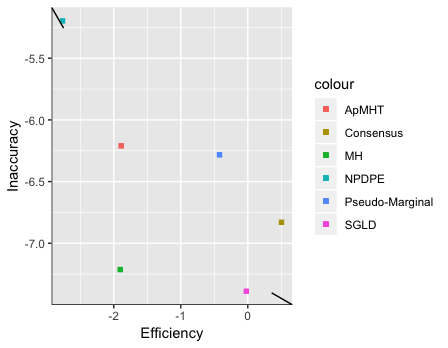
\includegraphics[resolution=110]{DGP0_plots/DGP0_HD_ESS.png}

\end{figure}
\newgeometry{top=5mm}

\begin{figure}
\caption{Summary plots}
\label{plots_DGP0}
\centering
\subfloat[ApMHT diagnostics]{
  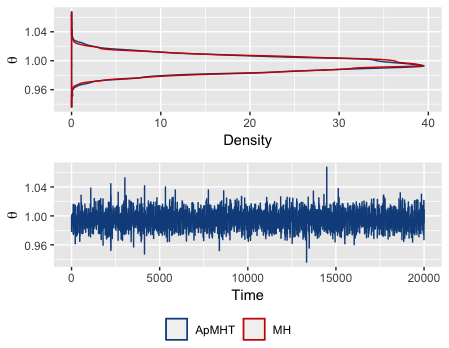
\includegraphics[resolution=160]{DGP0_plots/DGP0_diag_korattikara.png}
}
\subfloat[ApMHT \cite{geweke2004getting}'s test, p-value=0.63]{
  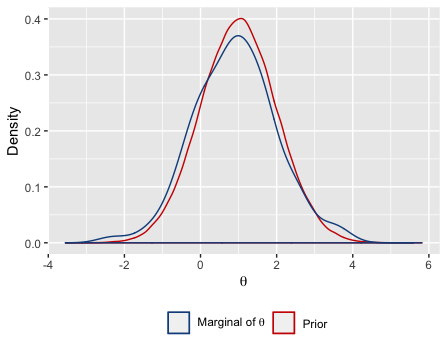
\includegraphics[resolution=160]{DGP0_plots/DGP0_GIT_korattikara.png}
}
\hspace{0mm}
\subfloat[Pseudo-Marginal diagnostics]{
  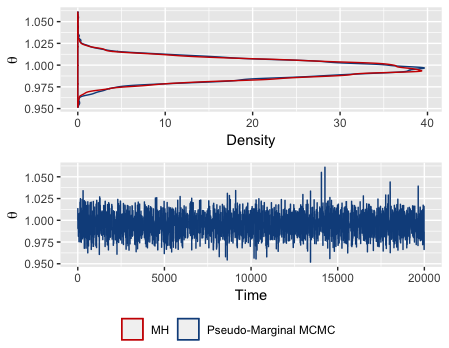
\includegraphics[resolution=160]{DGP0_plots/DGP0_diag_quiroz.png}
}
\subfloat[PM \cite{geweke2004getting}'s test, p-value=0.13]{
  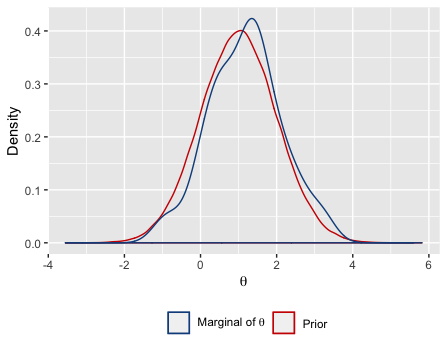
\includegraphics[resolution=160]{DGP0_plots/DGP0_GIT_quiroz.png}
}
\hspace{0mm}
\subfloat[SGLD diagnostics]{   % ???
  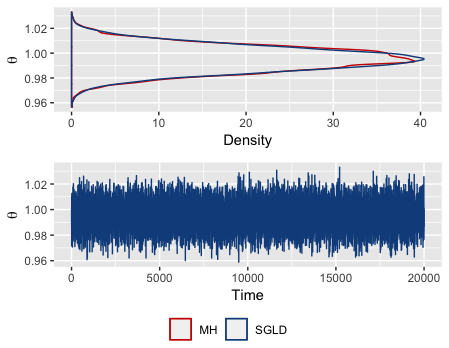
\includegraphics[resolution=160]{DGP0_plots/DGP0_diag_SGLD.png}
}
\subfloat[SGLD \cite{geweke2004getting}'s test, p-value=0.77]{
  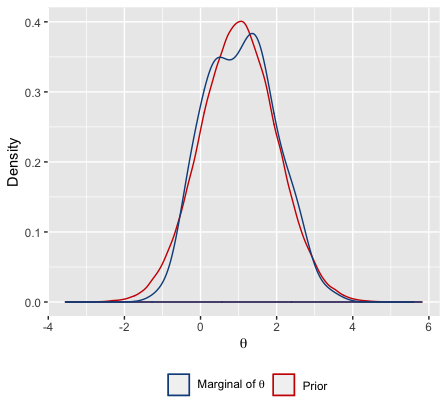
\includegraphics[resolution=160]{DGP0_plots/DGP0_GIT_SGLD.png}
}
\hspace{0mm}
\subfloat[Consensus diagnostics]{   % ???
  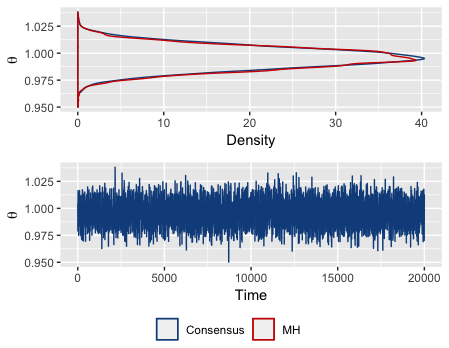
\includegraphics[resolution=160]{DGP0_plots/DGP0_diag_consensus.png}
}
\subfloat[Consensus \cite{geweke2004getting}'s test, p-value=0.20]{
  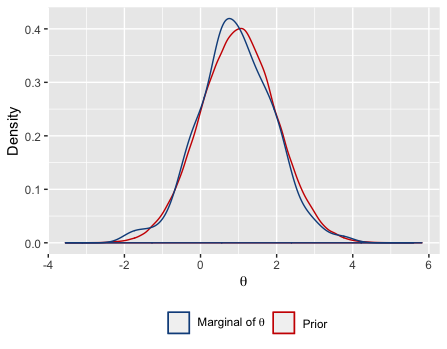
\includegraphics[resolution=160]{DGP0_plots/DGP0_GIT_consensus.png}
}
\end{figure}
\restoregeometry


\begin{figure}[H]
\ContinuedFloat
\caption{continued}
\centering
\subfloat[NPDPE diagnostics]{   % ???
  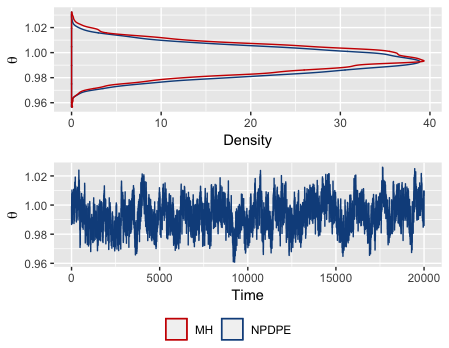
\includegraphics[resolution=160]{DGP0_plots/DGP0_diag_neiswanger.png}
}
\subfloat[NPDPE \cite{geweke2004getting}'s test, p-value=0.72]{
  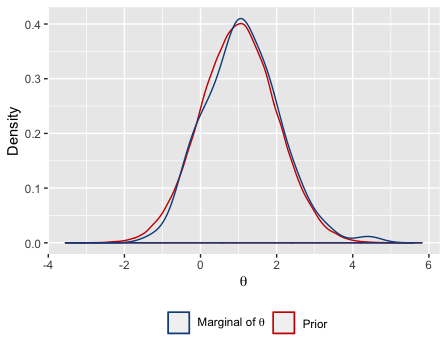
\includegraphics[resolution=160]{DGP0_plots/DGP0_GIT_neiswanger.png}
}
\end{figure}


\section{Bimodal - High variance}
\label{DGP2}

In this section, we wish to design a model whose posterior distribution is bimodal such that the probability density between the two modes is not too low. Since normality does not hold in this case, we can test the adaptability of Consensus Monte-Carlo which relies heavily on this assumption. It will also be interesting to see whether gradient methods like SGLD are able to mix properly or if, on the contrary, they will get stuck in one of the modes. More generally, this model should be a challenge to the mixing abilities of our algorithms.
\subsection{Data Generating Process}

The model considered is constructed as follows

\begin{align}
\label{eq:1}
&p(z_i|\theta)=\mathcal N(z_i;|\theta|,\sigma^2),\text{ for $i=1,...,N$}&\text{Likelihood}\\
\label{eq:2}
&\pi(\theta)=\mathcal N(\theta;0,s^2)&\text{Prior distribution}
\end{align}
Where $\sigma^2$=20 and $s^2=0.3^2$.

Hence, the posterior given one observation $z_i$ is of the form

\begin{align*}
\pi(\theta|z_i)&\propto \exp\left\{-\frac{1}{\sigma^2}(z_i-|\theta|)^2\right\}\times\exp\left\{-\frac{|\theta|^2}{2s^2}\right\}\\
&\propto \exp\left\{-\frac{(1+\frac{\sigma^2}{s^2})}{2}(|\theta|-(1+\frac{\sigma^2}{s^2})^{-1}z_i)^2\right\}
\end{align*}

which is bimodal in $\theta$ with the two modes being symmetric around 0. We choose $\theta=0.1$ so that the area of low posterior probability between the two modes is not too large to prevent good mixing. 
For this model we set $T=20000$ and the data set size $N=10000$.

\subsection{Results}
We attempt to tune each algorithm's parameters so that their Hellinger distance from the true posterior is below $0.01$. As can be seen in Table \ref{tab1} we did not manage to tune SGLD parameter $\varepsilon$ in order to achieve this goal but the Hellinger distance for this algorithm can be considered close enough. On the contrary, some algorithms like Pseudo-marginal MCMC are quite far below the chosen threshold.\\
As can be seen on Figure \ref{plots_DGP2}, all algorithms have successfully passed \cite{geweke2004getting}'s test except Consensus Monte-Carlo. This could be expected as the technique derived by \cite{scott2016bayes} relies heavily on the assumption that normality holds, which is clearly not the case here. Conversely, its parallel counterpart NPDPE seems to have worked in a better way probably thanks to its non-parametric property. 
Surprisingly, SGLD does seem to have made a good approximation of the true posterior, although we expected it to get stuck in one of the modes.\\
The trace plots indicate rather good mixing even though NPDPE's performance in that matter seems weaker.\\
When we look at the number of standardised likelihood evaluations we see that Pseudo-Marginal MCMC is undeniably more efficient. When it comes to $ESS$, we can spot no real outlier although we should highlight the rather poor performance of NPDPE, which we could already infer from the trace plot.\\
Overall, when looking at the $ESS$ per standardised likelihood evaluation, it is clear that Pseudo-Marginal MCMC outperformed the other algorithms on this synthetic data set.
\begin{table}[H]
    \centering
    \caption{Summary}
    \label{tab1}
    \begin{tabular}{ccccc}
\hline
&Parameter &\cite{geweke2004getting}'s & Hellinger & $ESS$/\\
&tuning&test :&distance&std. likelihood\\
&&  Fail/Pass &  from \textit{true posterior} &    evaluation\\

\hline
MH &-& - & 0.0012 & $\frac{2627.75}{20000}=0.13$ \\
&&&&\\
\hline
ApMHT &$\varepsilon=0.05$& Pass & $0.0018$ & $\frac{2589.55}{19130.2}=0.14$ \\
&&&&\\
\hline
Pseudo-marginal &m=100& Pass & $0.00083$ &$\frac{1614.1}{3120}=0.52$\\
&K=190&&&\\
\hline
SGLD &$\varepsilon=0.05$& Pass & $0.012$ & $\frac{1361.1}{20000}=0.07$\\
&m=5000&&&\\
\hline
Consensus MC &M=10& Fail & $0.086$* & $\frac{2418.326}{2000}=1.21$*\\
&&&&\\
\hline
NPDPE &M=10& Pass & $0.0012$&$\frac{306.97}{2000}=0.15$\\
&h=0.1&&&\\
\hline
\end{tabular}
\small{*These values are not relevant as the algorithm did not pass \cite{geweke2004getting}'s test.}
\end{table}

\begin{figure}[H]
\caption{Log of Hellinger distance vs log of ESS per std. likelihood evaluation}
\centering

  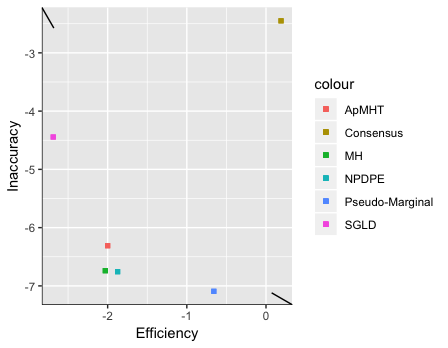
\includegraphics[resolution=110]{DGP2_plots/DGP2_HD_ESS.png}

\end{figure}

\newgeometry{top=5mm}

\begin{figure}
\caption{Summary plots}
\label{plots_DGP2}
\centering
\subfloat[ApMHT diagnostics]{
  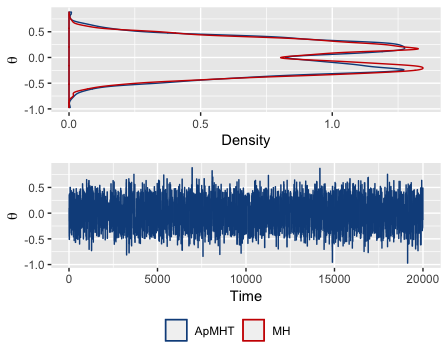
\includegraphics[resolution=160]{DGP2_plots/DGP2_diag_korattikara.png}
}
\subfloat[ApMHT \cite{geweke2004getting}'s test, p-value=0.97]{
  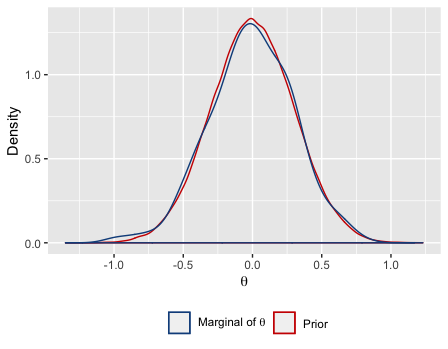
\includegraphics[resolution=160]{DGP2_plots/DGP2_GIT_korattikara.png}
}
\hspace{0mm}
\subfloat[Pseudo-Marginal diagnostics]{
  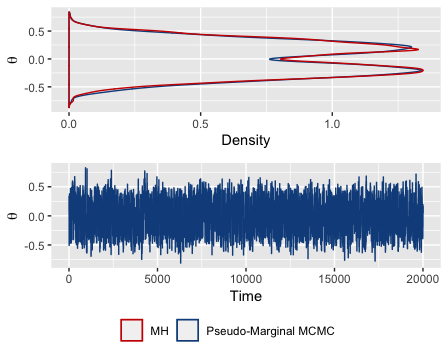
\includegraphics[resolution=160]{DGP2_plots/DGP2_diag_quiroz.png}
}
\subfloat[PM \cite{geweke2004getting}'s test, p-value=0.17]{
  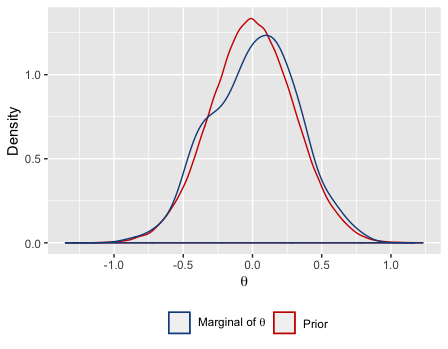
\includegraphics[resolution=160]{DGP2_plots/DGP2_GIT_quiroz.png}
}
\hspace{0mm}
\subfloat[SGLD diagnostics]{   % ???
  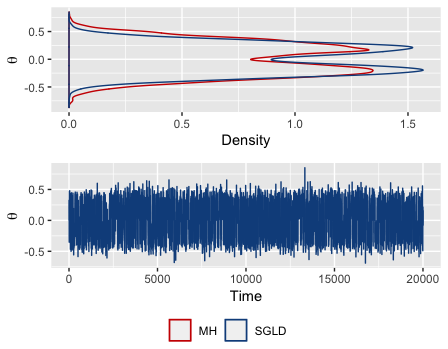
\includegraphics[resolution=160]{DGP2_plots/DGP2_diag_SGLD.png}
}
\subfloat[SGLD \cite{geweke2004getting}'s test, p-value=0.89]{
  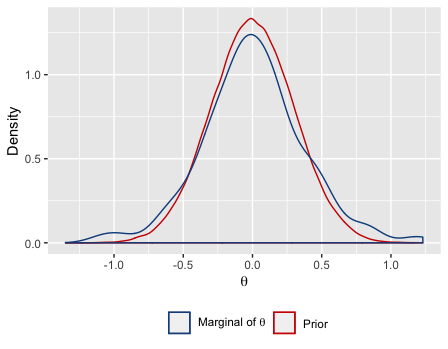
\includegraphics[resolution=160]{DGP2_plots/DGP2_GIT_SGLD.png}
}
\hspace{0mm}
\subfloat[Consensus diagnostics]{   % ???
  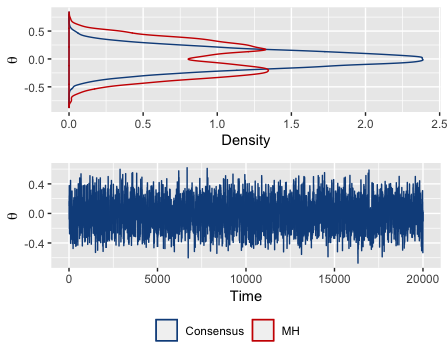
\includegraphics[resolution=160]{DGP2_plots/DGP2_diag_consensus.png}
}
\subfloat[Consensus \cite{geweke2004getting}'s test, p-value=0]{
  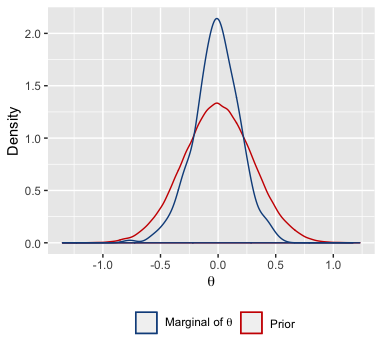
\includegraphics[resolution=160]{DGP2_plots/DGP2_GIT_consensus.png}
}
\end{figure}
\restoregeometry


\begin{figure}[H]
\ContinuedFloat
\caption{continued}
\centering
\subfloat[NPDPE diagnostics]{   % ???
  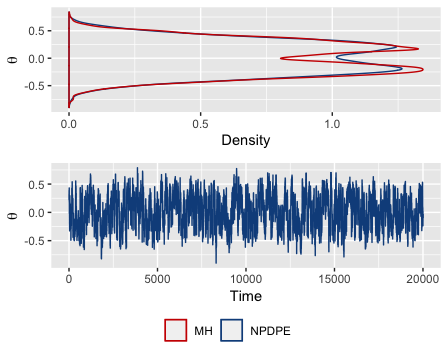
\includegraphics[resolution=160]{DGP2_plots/DGP2_diag_neiswanger.png}
}
\subfloat[NPDPE \cite{geweke2004getting}'s test, p-value=0.92]{
  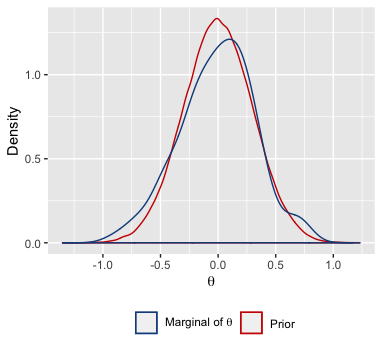
\includegraphics[resolution=160]{DGP2_plots/DGP2_GIT_neiswanger.png}
}
\end{figure}




\section{Bimodal - Low variance}
\label{DGP1}
In this section, we repeat a similar experiment of bimodality. However, we truly separate the modes by an area of low probability. This should pose a true challenge for MCMC algorithms that do not propose new candidates according to a random walk as they may not be able to cross this artificial low porobability "bridge". In particular, it will be interesting to see how SGLD, which performed surprinsingly well in the previous experiment, cope with this situation.
\subsection{Data Generating Process}

We repeat the scheme of the previous section setting this time $\sigma^2=1$. Thanks to this trick, the posterior distribution should be much more concentrated around the modes.
\begin{align}
\label{eq:5}
&p(z_i|\theta)=\mathcal N(z_i;|\theta|,\sigma^2),\text{ for $i=1,...,N$}&\text{Likelihood}\\
\label{eq:6}
&\pi(\theta)=\mathcal N(\theta;0,s^2)&\text{Prior distribution}
\end{align}
Where $\sigma^2$=1 and $s^2=0.3^2$.
For this model we set $T=20000$ and the data set size $N=10000$
\subsection{Results}
Figure \ref{plot:bimod} indicates that ApMHT and Pseudo-marginal MCMC seem to give the best approximations of the true posterior. They are also the only two methods that successfully pass \cite{geweke2004getting}'s test.\\
As to the other algorithms, we can see that, as feared, SGLD got stuck in one mode whereas consensus Monte-Carlo unsurprisingly produced an erroneous approximation based on the Bernstein-von Mises theorem. However, we can see that NPDPE almost succeeded in approximating the two mode-scheme but clearly overestimated the variance of the posterior.
When ignoring the algorithms which did not converge to the posterior, Table \ref{tab2} and Figure \ref{HD2} show a clear dominance of Pseudo-Marginal MCMC both in terms of quality of approximation and efficiency, followed by ApMHT. Both algorithms yield an equal or better Hellinger distance to the posterior than MH and a substantially higher ESS per std. likelihood evaluation.
\begin{table}
    \centering
    \caption{Summary}
    \label{tab2}
    \begin{tabular}{ccccc}
\hline
&Parameter &\cite{geweke2004getting}'s & Hellinger & $ESS$/\\
&tuning&test :&distance&std. likelihood\\
&&  Fail/Pass &  from \textit{true posterior} &    evaluation\\

\hline
MH &-& - & 0.013 & $\frac{20.72}{20000}=0.001$ \\
&&&&\\
\hline
ApMHT &$\varepsilon=0.05$& Pass & $0.016$ & $\frac{125.56}{26537}=0.005$ \\
&&&&\\
\hline
Pseudo-marginal &m=200& Pass & $0.003$ &$\frac{168.08}{3632}=0.046$\\
&K=54&&&\\
\hline
SGLD &$\varepsilon=2.25*10^{-4}$& Fail &0.31&$\frac{25588.15}{20000}=1.28$*\\
&m=5000&&&\\
\hline
Consensus MC &M=3& Fail & 0.83 & $\frac{2031.54}{6666}=0.30$*\\
&&&&\\
\hline
NPDPE &M=3& Fail &0.25&$\frac{1609.33}{6666}=0.24$*\\
&h=0.07&&&\\
\hline
\end{tabular}
\small{*These values are not relevant as the algorithm did not pass \cite{geweke2004getting}'s test.}
\end{table}

\begin{figure}
\caption{Log of Hellinger distance vs log of ESS per std. likelihood evaluation}
\label{HD2}
\centering

  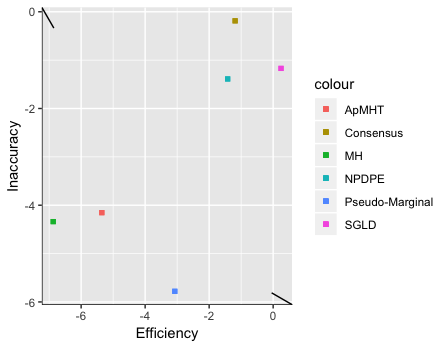
\includegraphics[resolution=110]{bimod_plots/bimod_HD_ESS.png}

\end{figure}

\newgeometry{top=5mm}

\begin{figure}
\caption{Summary plots}
\label{plot:bimod}
\centering
\subfloat[ApMHT diagnostics]{
  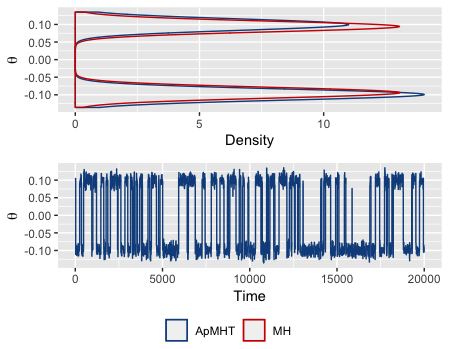
\includegraphics[resolution=160]{bimod_plots/bimod_diag_korattikara.png}
}
\subfloat[ApMHT \cite{geweke2004getting}'s test, p-value=0.37]{
  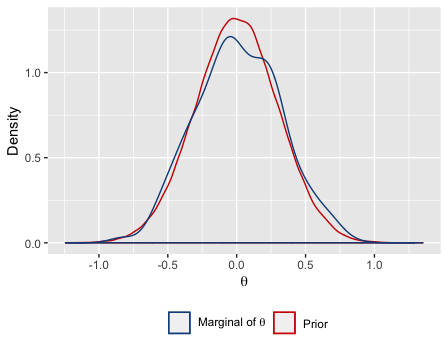
\includegraphics[resolution=160]{bimod_plots/bimod_GIT_korattikara.png}
}
\hspace{0mm}
\subfloat[Pseudo-Marginal diagnostics]{
  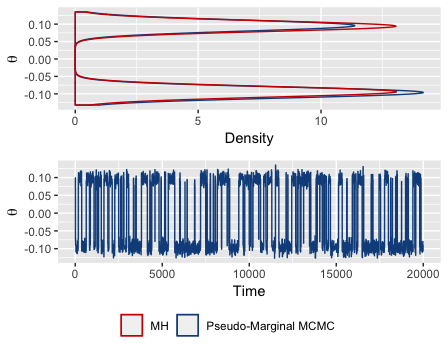
\includegraphics[resolution=160]{bimod_plots/bimod_diag_quiroz.png}
}
\subfloat[PM \cite{geweke2004getting}'s test, p-value=0.88]{
  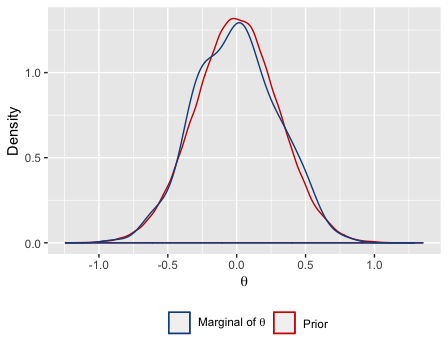
\includegraphics[resolution=160]{bimod_plots/bimod_GIT_quiroz.png}
}
\hspace{0mm}
\subfloat[SGLD diagnostics]{   % ???
  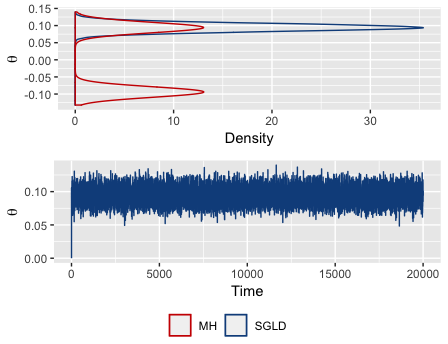
\includegraphics[resolution=160]{bimod_plots/bimod_diag_SGLD.png}
}
\subfloat[SGLD \cite{geweke2004getting}'s test, p-value=0]{
  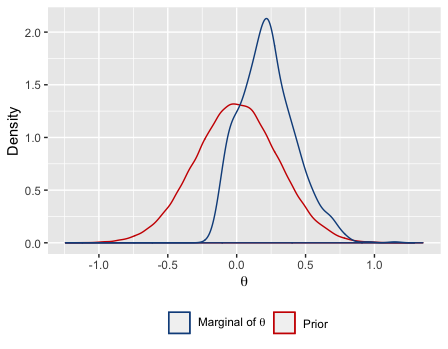
\includegraphics[resolution=160]{bimod_plots/bimod_GIT_SGLD.png}
}
\hspace{0mm}
\subfloat[Consensus diagnostics]{   % ???
  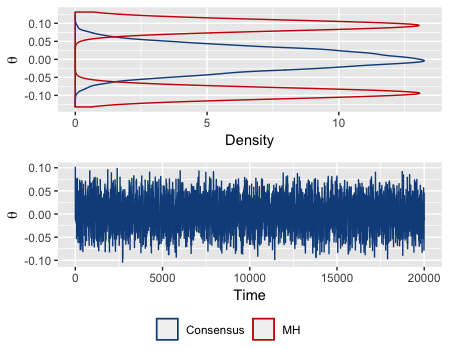
\includegraphics[resolution=160]{bimod_plots/bimod_diag_consensus.png}
}
\subfloat[Consensus \cite{geweke2004getting}'s test, p-value=0]{
  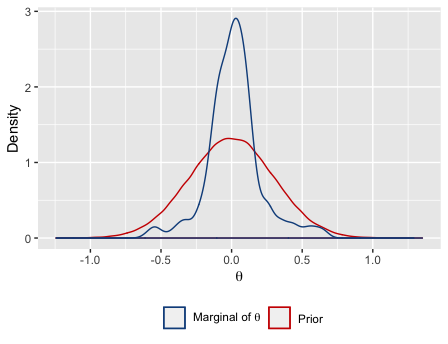
\includegraphics[resolution=160]{bimod_plots/bimod_GIT_consensus.png}
}
\end{figure}
\restoregeometry


\begin{figure}[H]
\ContinuedFloat
\caption{continued}
\centering
\subfloat[NPDPE diagnostics]{   % ???
  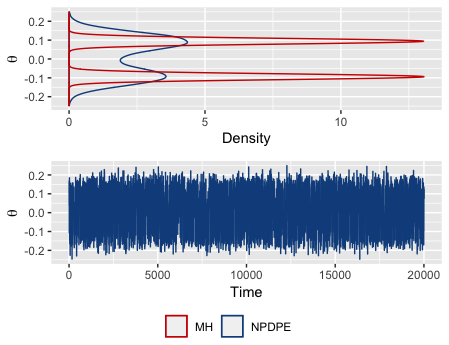
\includegraphics[resolution=160]{bimod_plots/bimod_diag_neiswanger.png}
}
\subfloat[NPDPE \cite{geweke2004getting}'s test, p-value=0]{
  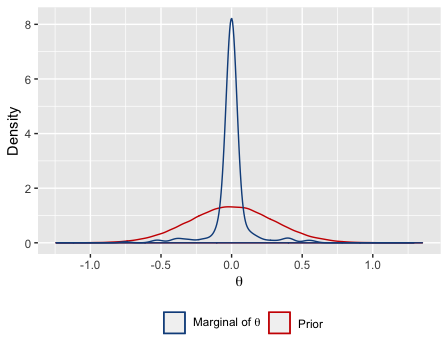
\includegraphics[resolution=160]{bimod_plots/bimod_GIT_neiswanger.png}
}
\end{figure}


\section{High-dimensional logistic regression}
This final experiment will give us a more concrete insight into real world problems as we will now consider a fairly high dimensional logistic regression with a relatively low amount of data. It might seem surprising to set $N=1000$ when our main interest are tall data sets but we wished to reflect the common situation when the number of parameters to estimate, in our case 20, combined with a 'small' amount of data makes accurate inference difficult to achieve. However, the conclusions we will draw from this experiment can easily be extended to situations where say $N=100000$ and the number of parameters is $d=1000$.\\
This setting also enables us to confront our algorithms with rather fat-tailed posterior distribution, which has not been done previously. In such situations we expect mixing to be difficult for the algorithms which propose updates according to a random walk, even with a large step-size. 

\subsection{Data Generating Process}
In this section, we artificially create a logistic regression setting. To do so, we first sample our true parameters as follows,
$$\theta\sim\mathcal N_d(0,1)$$
where $d=20$.\\
We then generate the covariates $x_i=(x_{1i},...,x_{20i})$ for $i=1,...,1000$ each independently from a standard Normal distribution.\\
Finally, $$z_i\sim \mathcal{B}(\pi_i)$$ where $$\pi_i=\frac{e^{\theta_1x_{1i}+...+\theta_{20}x_{20i}}}{1+e^{\theta_1x_{1i}+...+\theta_20x_{20i}}}$$
and $\mathcal{B}(\pi_i)$ denotes the Bernoulli distribution of mean $\pi_i$.\\
For this experiment, we choose to set $T=20000$ and simulate our \textit{true posterior} from 2,000,000 runs of standard random-walk MH. Moreover, we choose the prior distribution $\pi$ to be standard multivariate normal.

\subsection{Results}
So as to provide clear and meaningful plots, Figure \ref{plots_DGP3} shows contour lines of the marginal distributions of $\theta_2$ and $\theta_4$ only, and all other measures of assessment including \cite{geweke2004getting}'s test are carried out on the marginal distribution of $\theta_2$.
As can be seen on the summary plots (Figure \ref{plots_DGP3}) most algorithms seem to have produced a good enough approximation of the true posterior, even though the marginals sampled by NPDPE look somewhat shifted. Nevertheless, all \cite{geweke2004getting}'s tests suggest that samples were indeed drawn from the posterior distribution.  
Overall, Table \ref{tab3} and Figure \ref{HD3} show very strong performances in term of approximation and efficiency for SGLD when compared to its counterparts. The facts that the mixing of all other algorithms is poorer tends to indicate that another proposal distribution should be used instead of a random walk. In particular, a Langevin proposal might be more efficient, as suggested by the achievements of SGLD. Therefore, we cannot discard these algorithms as their performances might be enhanced by a more suitable choice of proposal distribution.


\label{DGP3}
\begin{table}[H]
    \centering
    \caption{Summary}
    \label{tab3}
    \begin{tabular}{ccccc}
\hline
&Parameter &\cite{geweke2004getting}'s & Hellinger & $ESS$/\\
&tuning&test :&distance&std. likelihood\\
&&  Fail/Pass &  from \textit{true posterior} &    evaluation\\

\hline
MH &-& - & 0.0024 & $\frac{273.50}{20000}=0.014$ \\
&&&&\\
\hline
ApMHT &$\varepsilon=0.05$& Pass & $0.0054$ & $\frac{273.70}{25840.8}=0.011$ \\
&&&&\\
\hline
Pseudo-marginal &m=100& Pass & $0.0027$ &$\frac{185.10}{28240}=0.0066$\\
&K=153&&&\\
\hline
SGLD &$\varepsilon=0.022$& Pass &0.00042&$\frac{20685.87}{20000}=1.03$\\
&m=500&&&\\
\hline
Consensus MC &M=3& Pass & $0.015$ & $\frac{375.23}{6660}=0.056$\\
&&&&\\
\hline
NPDPE &M=3& Pass &0.025&$\frac{510.05}{6660}=0.077$\\
&h=0.07&&&
\end{tabular}
\end{table}

\begin{figure}[H]
\caption{Log of Hellinger distance vs log of ESS per std. likelihood evaluation}
\label{HD3}
\centering

  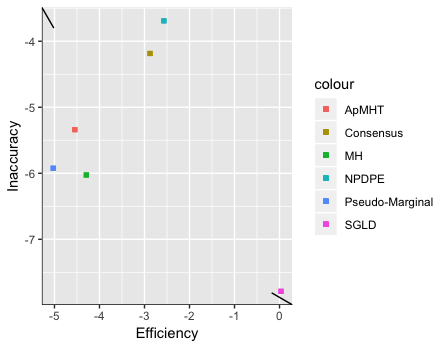
\includegraphics[resolution=110]{DGP3_plots/DGP3_HD_ESS.png}

\end{figure}
\newgeometry{top=5mm}

\begin{figure}
\caption{Summary plots}
\label{plots_DGP3}
\centering
\subfloat[ApMHT diagnostics]{
  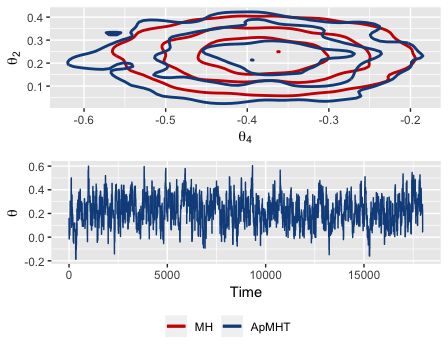
\includegraphics[resolution=160]{DGP3_plots/DGP3_diag_korattikara.png}
}
\subfloat[ApMHT \cite{geweke2004getting}'s test, p-value=0.50]{
  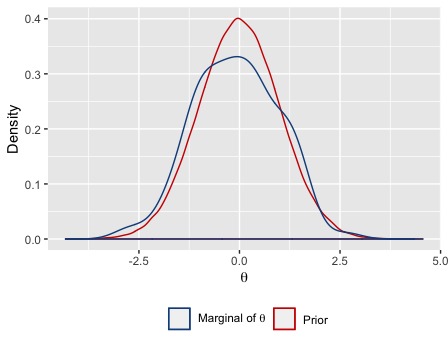
\includegraphics[resolution=160]{DGP3_plots/DGP3_GIT_korattikara.png}
}
\hspace{0mm}
\subfloat[Pseudo-Marginal diagnostics]{
  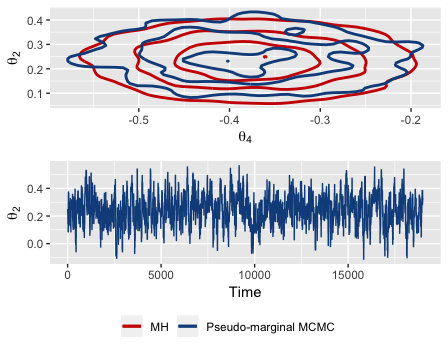
\includegraphics[resolution=160]{DGP3_plots/DGP3_diag_quiroz.png}
}
\subfloat[PM \cite{geweke2004getting}'s test, p-value=0.23]{
  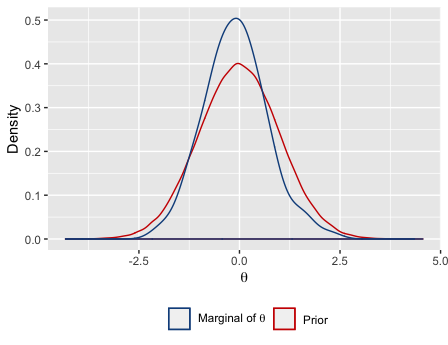
\includegraphics[resolution=160]{DGP3_plots/DGP3_GIT_quiroz.png}
}
\hspace{0mm}
\subfloat[SGLD diagnostics]{   % ???
  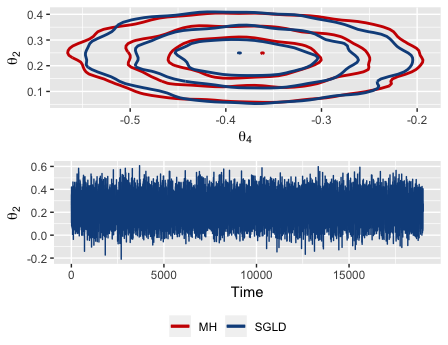
\includegraphics[resolution=160]{DGP3_plots/DGP3_diag_SGLD.png}
}
\subfloat[SGLD \cite{geweke2004getting}'s test, p-value=0.26]{
  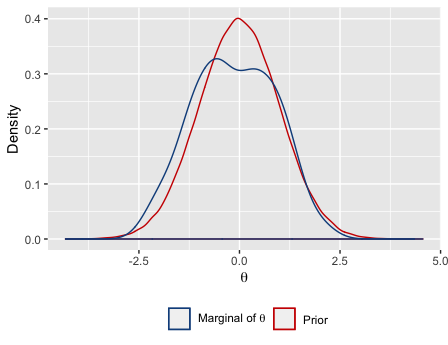
\includegraphics[resolution=160]{DGP3_plots/DGP3_GIT_SGLD.png}
}
\hspace{0mm}
\subfloat[Consensus diagnostics]{   % ???
  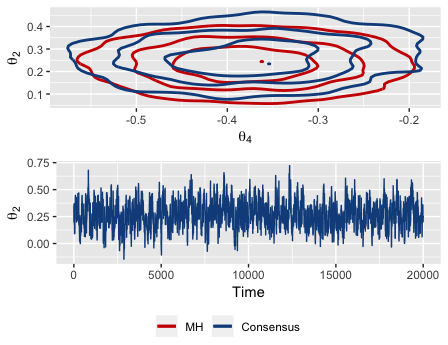
\includegraphics[resolution=160]{DGP3_plots/DGP3_diag_consensus.png}
}
\subfloat[Consensus \cite{geweke2004getting}'s test, p-value=0.72]{
  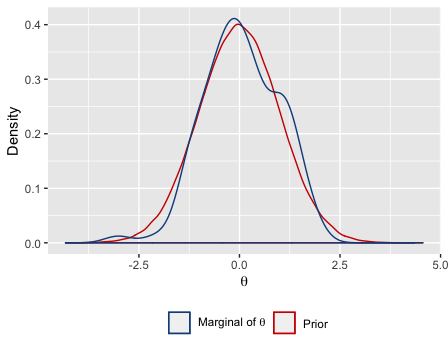
\includegraphics[resolution=160]{DGP3_plots/DGP3_GIT_consensus.png}
}
\end{figure}
\restoregeometry


\begin{figure}[H]
\ContinuedFloat
\caption{continued}
\centering
\subfloat[NPDPE diagnostics]{   % ???
  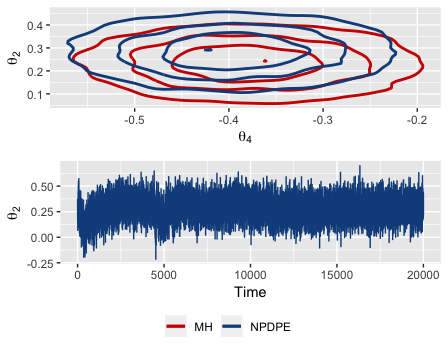
\includegraphics[resolution=160]{DGP3_plots/DGP3_diag_neiswanger.png}
}
\subfloat[NPDPE \cite{geweke2004getting}'s test, p-value=0.17]{
  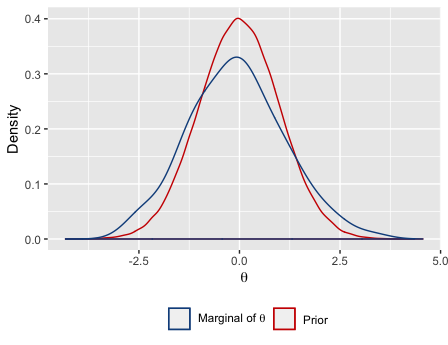
\includegraphics[resolution=160]{DGP3_plots/DGP3_GIT_neiswanger.png}
}
\end{figure}




\chapter*{Conclusions and future work}
\addcontentsline{toc}{chapter}{Conclusions and future work}
\section*{Conclusions}
\addcontentsline{toc}{section}{Conclusions}

During this study, we have been able to implement several recent algorithms designed to improve traditional MCMC methods when confronted to tall data sets in a sample Bayesian setting. The different experiments we carried out led us to the following conclusions.\\

Consensus Monte Carlo is a very easy algorithm to implement which performs surprisingly well, providing some conditions are met. It indeed turned out to be very dependent on the assumption that the Bernstein-Von Mises theorem holds. When this condition is satisfied, it generally outperforms most of its counterparts in terms of ESS per std likelihood evaluation, even though its approximation error is usually slightly higher. On the other hand, more complex frameworks such as bimodality really hindered a correct posterior sampling. Therefore, we highly recommend its use for simple models especially if the user has access to a high number of computational units. In our examples, we set $M=3$ as typical laptops will have either 2 or 4 cores (assuming they cannot run more than 1 thread at a time). However, one can easily imagine implementing the algorithm with large values of $M$, which would improve efficiency even more.\\

We picked our second \textit{divide and conquer} algorithm, NPDPE, as a more flexible alternative to Consensus Monte Carlo. Despite its tedious implementation, this method did prove itself able to adapt to more scenarios than its other parallel counterpart and only failed the \cite{geweke2004getting}'s test once in the context of an extreme experimental design. Although it has suffered from poor mixing and relatively high approximation errors, the last experiment showed its ability to perform well where the other methods experienced difficulties. As for consensus Monte Carlo, its number of required likelihood evaluations makes it a mighty tool when confronted to large data sets.\\

SGLD, a rejection-free algorithm, was our only algorithm whose proposal distribution moved along the gradient of the posterior distribution. Thus, we had concerns as to its ability to mix properly when confronted to multimodality or posteriors with a complex geometry. However, this simple algorithm performed remarkably well on our first bimodal example as it succeeded not to get trapped in one of the modes, although its efficiency was not among the best. Moreover, it outperformed by far the other methods on the logistic regression experiment, both in terms of approximation error (beating Metropolis-Hastings itself) and of ESS per std likelihood evaluations. Its performances on our test data set were also remarkable.\\

Pseudo-marginal MCMC is probably the most consistent and reliable algorithm we have implemented. It passed the \cite{geweke2004getting}'s test for all experiments and yielded the best approximation error and ESS per std likelihood evaluation for both our bimodal experimental settings. Its poorer mixing on the last experiment would probably be improved with a more suitable choice of proposal distribution. Its downside however is that it requires to derive the gradient and Hessian matrix of the likelihood function evaluated at the data analytically. If those quantities had to be computed numerically, one should expect a high increase in the number of required likelihood evaluations.\\

Finally, ApMHT, which is a rather intuitive algorithm, showed it had a great adaptability to most situations. Like for Pseudo-marginal MCMC, no test suggested that it did not sample from the posterior distribution. Although it has never been the top-performing algorithm, it showed great consistency across the different synthetic models we designed. However, MH sometimes proved itself more efficient than ApMHT.\\

We sum up all our conclusions in Table \ref{tab:final} where we mention the principal features of each algorithm and also provide a personal feeling regarding the level of difficulty of implementation for each method.

\section*{Future work}
\addcontentsline{toc}{section}{Future work}
Throughout our analysis, we tried to give a useful insight into how modern MCMC techniques could tackle the challenges Bayesian inference has been facing since the advent of Big Data. \\
Some additional content might have been interesting to provide. In particular, it would be interesting to know whether the number of required likelihood evaluations is a linear or sub-linear function of the data set size $N$. To give a simple overview of the situation, we provide Figure \ref{plot:final}. These curves were derived using our first model (test data set) by using the number of likelihood evaluations indicated in Table \ref{tab:final} below. For Consensus Monte Carlo and NPDPE we assumed the user had M=10 machines available. By looking at our previous experiments' tuning parameters values we make the assumptions that $m=0.5N$ for SGLD and $K=0.05N$, $m=0.02N$ for Pseudo-Marginal MCMC. For ApMHT we had to run simulations for different values of $N$ as the number of likelihood evaluations is random.\\
Making these strong assumptions, we can see that only ApMHT's curve seems to be a sub-linear function of $N$. However the curves of SGLD and Pseudo-Marginal represent here a worst-case scenario as the values $m$ and $K$ should be tuned for each data set size $N$. Hence, some further work should be done in order to produce similar plots on different data sets, making sure that the parameters of each algorithm are properly tuned for each value of $N$.
\begin{figure}[H]
\caption{Log of Hellinger distance vs log of ESS per std. likelihood evaluation}
\label{plot:final}
\centering

  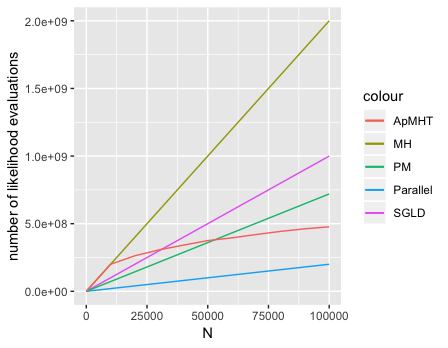
\includegraphics[resolution=110]{final_plot.png}

\end{figure}
One should also consider using different ways of proposing a candidate $\theta'$ for all the algorithms except SGLD. We have indeed seen in our last experiment that the choice of proposal distribution is essential for good mixing and satisfactory performances.\\

A lot of additional work out of the scope of this study could be carried out in order produce a complete overview of the current state of research in this domain. For instance, other recent approaches like the rejection-free Bouncy Particle Sampler by \cite{bouchard2017bouncy} samples exactly from the posterior distribution and shows really promising results.\\
One should also consider comparing the MCMC methods we implemented to other popular tools designed to perform approximate Bayesian inference like Variational inference (e.g \cite{jain2018variational}) or Expectation propagation (see \cite{minka2001expectation}).\\


\afterpage{%
    \clearpage% Flush earlier floats (otherwise order might not be correct)
    \thispagestyle{empty}% empty page style (?)
    \begin{landscape}% Landscape page
        \centering % Center table
        \vspace*{-2.5cm}
        \captionof{table}{Summary table}% Add 'table' caption
        \label{tab:final}
        \begin{tabular}{c|ccccc}
         & ApMHT (RW) & Pseudo-Marginal (RW) & SGLD & Consensus (RW) & NPDPE (RW)  \\
        \hline
        Exact posterior  &Approximate & Approximate& Approximate& Asym. exact & Approximate\\
         sampling ?& Asym. exact as $\varepsilon\rightarrow0$ & Asym. exact as $m\rightarrow N$&
         Asym. exact as $m\rightarrow N$&if B-vM theorem holds\\
         \hline
         Number of likelihood& random & $T(4K+8m)$* & $Tm$*& $TN/M$ &$TN/M$\\
         evaluations\\
        \hline
        Difficulty of &Easy&Difficult*&Medium*&Easy&Medium\\
        implementation\\
        \hline
        \hline
        Normal & AE** = $4^{th}$ & AE=$3^{rd}$&AE =$1^{st}$&AE =$2^{nd}$&AE =$5^{th}$\\
        model&ESS/llik*** = $4^{th}$ & ESS/llik=$3^{rd}$&ESS/llik =$2^{nd}$&ESS/llik =$1^{st}$&ESS/llik =$5^{th}$\\
        \hline
        Bimodal model & AE = $3^{rd}$ & AE=$1^{st}$&AE =$4^{th}$&Fail&AE =$2^{nd}$\\
        high variance &ESS/llik = $3^{rd}$ & ESS/llik=$1^{st}$&ESS/llik =$4^{th}$&&ESS/llik =$2^{rd}$\\
        \hline
        Bimodal model & AE = $2^{nd}$ & AE=$1^{st}$&Fail&Fail&Fail\\
        low variance &ESS/llik = $2^{nd}$ & ESS/llik=$1^{st}$&&&\\
        \hline
         High dimensional& AE = $3^{rd}$ & AE=$2^{nd}$&AE =$1^{st}$&AE =$4^{nd}$&AE =$5^{th}$\\
        logistic reg. model&ESS/llik = $4^{th}$ & ESS/llik=$5^{th}$&ESS/llik =$1^{st}$&ESS/llik =$3^{rd}$&ESS/llik =$2^{nd}$\\
        \hline
    \end{tabular}
        \small{*Assuming the gradient and the Hessian matrix are computed analytically\\}
        \small{**Ranking of the algorithms according to their ability to minimize the approximation error (AE)\\}
        \small{***Ranking of the algorithms according to their ability to maximise the ESS per std likelihood evaluation (ESS/llik)\\}
    \end{landscape}
    \clearpage% Flush page
}
\restoregeometry
\bibliography{ref} 
\bibliographystyle{apa}

\addcontentsline{toc}{chapter}{Appendix}

\begin{appendix}
\chapter{Miscellaneous}
\section{Proof of theorem \ref{th:1} by \cite{korattikara2014austerity}}

Following is a screenshot of the proof provided by \cite{korattikara2014austerity} in their article. The Markov transition kernel they define seems to be wrong as it should be equal to 
$$P_a(\theta,\theta')q(\theta'|\theta)+\left(1-\int_{\theta'}P_a(\theta,\theta')q(\theta'|\theta)d\theta'\right)\delta_{\theta}(\theta')$$ following the notation of the authors.\\ 
This mistake changes the proof dramatically but the obtained result is the same, as we have shown.
\begin{figure}[H]
    \centering
    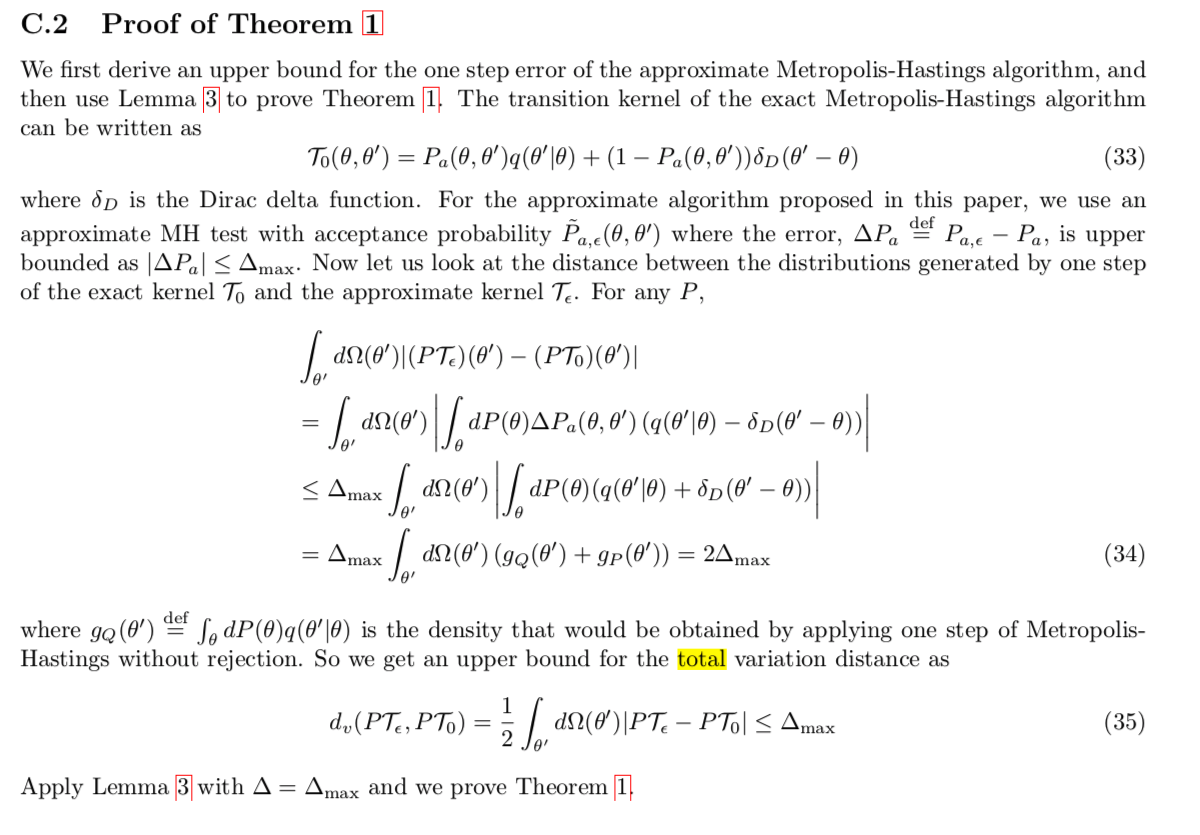
\includegraphics[resolution=200]{korattikara_proof.png}
    \caption{Screenshot of the proof of Theorem \ref{th:1} as given by \cite{korattikara2014austerity}}
    \label{fig:korattikara_appendix}
\end{figure}

\section{Derivation of the Gradient and Hessian matrix for GLM by \cite{quiroz2018speeding}}
In their appendix, \cite{quiroz2018speeding} give an indication on how to compute the control variates for a Generalised Linear Model (GLM). However, it seems like their derivation of the gradient function is wrong.\\
Using the notation of the original article (cf Figure \ref{fig:quirow_appendix}) we indeed find that 
\begin{align}
    \frac{\partial l}{\partial x}&=\frac{\theta k'^{-1}(x^T\theta)g'(\Psi)}{g(\Psi)}+T(y)\theta k'^{-1}(x^T\theta)b'(\Psi)\\
    &=\left(\frac{g'(\Psi)}{g(\Psi)}k'^{-1}(x^T\theta)+T(y) k'^{-1}(x^T\theta)b'(\Psi)\right)\theta
\end{align}
by applying the chain rule.
\begin{figure}
    \centering
    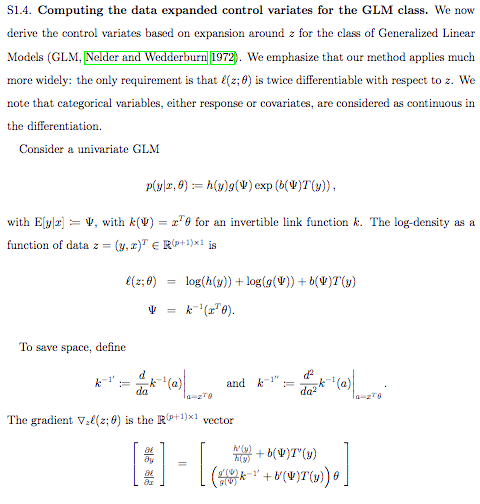
\includegraphics[resolution=100]{proof_quiroz.png}
    \caption{Screenshot of the appendix of \cite{quiroz2018speeding}}
    \label{fig:quirow_appendix}
\end{figure}
\chapter{R code}
\newgeometry{top=5mm, left=20mm, right=20mm}
\section{Libraries}
\begin{knitrout}
\definecolor{shadecolor}{rgb}{0.969, 0.969, 0.969}\color{fgcolor}\begin{kframe}
\begin{alltt}
\hlkwd{library}\hlstd{(mvtnorm)}
\hlkwd{library}\hlstd{(coda)}
\hlkwd{library}\hlstd{(ggpubr)}
\hlkwd{library}\hlstd{(coda)}
\hlkwd{library}\hlstd{(rootSolve)}
\hlkwd{library}\hlstd{(ggplot2)}
\hlkwd{library}\hlstd{(plyr)}
\end{alltt}
\end{kframe}
\end{knitrout}

\section {DGP 1 : Test data - Normal Model}
\subsection{Parameters}
\begin{knitrout}
\definecolor{shadecolor}{rgb}{0.969, 0.969, 0.969}\color{fgcolor}\begin{kframe}
\begin{alltt}
\hlstd{n}\hlkwb{=}\hlnum{1e4}
\hlstd{theta}\hlkwb{=}\hlnum{1}
\hlstd{y}\hlkwb{=}\hlkwd{rnorm}\hlstd{(n,theta)}
\hlstd{z}\hlkwb{=}\hlkwd{as.matrix}\hlstd{(y)}
\end{alltt}
\end{kframe}
\end{knitrout}
\subsection{DGP and model functions}
\begin{knitrout}
\definecolor{shadecolor}{rgb}{0.969, 0.969, 0.969}\color{fgcolor}\begin{kframe}
\begin{alltt}
\hlstd{llik}\hlkwb{<-}\hlkwa{function} \hlstd{(}\hlkwc{i}\hlstd{,}\hlkwc{z}\hlstd{,}\hlkwc{theta}\hlstd{) \{}
  \hlkwd{return}\hlstd{(}\hlkwd{dnorm}\hlstd{(z[i],}\hlkwc{mean}\hlstd{=theta,} \hlkwc{log}\hlstd{=}\hlnum{TRUE}\hlstd{))}
\hlstd{\}}
\hlcom{#likelihood for the Pseudo-marginal algorithn}
\hlstd{llik}\hlkwb{<-}\hlkwa{function} \hlstd{(}\hlkwc{z}\hlstd{,}\hlkwc{theta}\hlstd{) \{}
  \hlkwd{return}\hlstd{(}\hlkwd{dnorm}\hlstd{(z,}\hlkwc{mean}\hlstd{=theta,} \hlkwc{log}\hlstd{=}\hlnum{TRUE}\hlstd{))}
\hlstd{\}}
\hlstd{log_prior}\hlkwb{<-}\hlkwa{function}\hlstd{(}\hlkwc{theta}\hlstd{) \{}
  \hlkwd{return}\hlstd{(}\hlkwd{dnorm}\hlstd{(theta,}\hlkwc{mean}\hlstd{=}\hlnum{1}\hlstd{,} \hlkwc{sd}\hlstd{=}\hlnum{0.3}\hlstd{,}\hlkwc{log}\hlstd{=}\hlnum{TRUE}\hlstd{))}
\hlstd{\}}
\hlstd{gradient_llik}\hlkwb{<-}\hlkwa{function}\hlstd{(}\hlkwc{z}\hlstd{,}\hlkwc{theta}\hlstd{) \{}
  \hlkwd{return}\hlstd{(}\hlopt{-}\hlstd{(z}\hlopt{-}\hlstd{theta))}
\hlstd{\}}
\hlstd{hessian_llik}\hlkwb{<-}\hlkwa{function}\hlstd{(}\hlkwc{z}\hlstd{,}\hlkwc{theta}\hlstd{) \{}
  \hlkwd{return}\hlstd{(}\hlkwd{rep}\hlstd{(}\hlopt{-}\hlnum{1}\hlstd{,}\hlkwd{length}\hlstd{(z)))}
\hlstd{\}}
\end{alltt}
\end{kframe}
\end{knitrout}

\section {DGP 2 : Bimodal - High Variance}
\subsection{Parameters}
\begin{knitrout}
\definecolor{shadecolor}{rgb}{0.969, 0.969, 0.969}\color{fgcolor}\begin{kframe}
\begin{alltt}
\hlstd{theta}\hlkwb{=}\hlnum{0.1}
\hlstd{sigma}\hlkwb{=}\hlnum{20}
\hlstd{n}\hlkwb{=}\hlnum{1e4}
\end{alltt}
\end{kframe}
\end{knitrout}
\subsection{DGP and model functions}
\begin{knitrout}
\definecolor{shadecolor}{rgb}{0.969, 0.969, 0.969}\color{fgcolor}\begin{kframe}
\begin{alltt}
\hlstd{y}\hlkwb{=}\hlkwd{rnorm}\hlstd{(n,}\hlkwc{mean}\hlstd{=}\hlkwd{abs}\hlstd{(theta),sigma)}
\hlstd{z}\hlkwb{=}\hlkwd{as.matrix}\hlstd{(y)}
\hlstd{llik}\hlkwb{<-}\hlkwa{function} \hlstd{(}\hlkwc{i}\hlstd{,}\hlkwc{z}\hlstd{,}\hlkwc{theta}\hlstd{) \{}
  \hlkwd{return}\hlstd{(}\hlkwd{dnorm}\hlstd{(z[i],}\hlkwc{mean}\hlstd{=}\hlkwd{abs}\hlstd{(theta),sigma,} \hlkwc{log}\hlstd{=}\hlnum{TRUE}\hlstd{))}
\hlstd{\}}
\hlcom{#Likelihood for the Pseudo-Marginal algorithm}
\hlstd{llik}\hlkwb{<-}\hlkwa{function} \hlstd{(}\hlkwc{z}\hlstd{,}\hlkwc{theta}\hlstd{) \{}
  \hlkwd{return}\hlstd{(}\hlkwd{dnorm}\hlstd{(z,}\hlkwc{mean}\hlstd{=}\hlkwd{abs}\hlstd{(theta),} \hlkwc{sd}\hlstd{=sigma,} \hlkwc{log}\hlstd{=}\hlnum{TRUE}\hlstd{))}
\hlstd{\}}
\hlstd{log_prior}\hlkwb{<-}\hlkwa{function}\hlstd{(}\hlkwc{theta}\hlstd{) \{}
  \hlkwd{return}\hlstd{(}\hlkwd{dnorm}\hlstd{(theta,}\hlkwc{mean}\hlstd{=}\hlnum{0}\hlstd{,}\hlnum{0.3}\hlstd{,}\hlkwc{log}\hlstd{=T))}
\hlstd{\}}
\hlstd{gradient_llik}\hlkwb{<-}\hlkwa{function}\hlstd{(}\hlkwc{z}\hlstd{,}\hlkwc{theta}\hlstd{) \{}
  \hlkwd{return}\hlstd{(}\hlopt{-}\hlstd{(}\hlnum{1}\hlopt{/}\hlstd{sigma}\hlopt{^}\hlnum{2}\hlstd{)}\hlopt{*}\hlstd{(z}\hlopt{-}\hlkwd{abs}\hlstd{(theta)))}
\hlstd{\}}
\hlstd{hessian_llik}\hlkwb{<-}\hlkwa{function}\hlstd{(}\hlkwc{z}\hlstd{,}\hlkwc{theta}\hlstd{) \{}
  \hlkwd{return}\hlstd{(}\hlkwd{rep}\hlstd{(}\hlopt{-}\hlstd{(}\hlnum{1}\hlopt{/}\hlstd{sigma}\hlopt{^}\hlnum{2}\hlstd{),}\hlkwd{length}\hlstd{(z)))}
\hlstd{\}}
\end{alltt}
\end{kframe}
\end{knitrout}

\section{DGP 3 : Bimodal - Low variance}
\subsection{Parameters}
\begin{knitrout}
\definecolor{shadecolor}{rgb}{0.969, 0.969, 0.969}\color{fgcolor}\begin{kframe}
\begin{alltt}
\hlstd{theta}\hlkwb{=}\hlnum{0.1}
\hlstd{sigma}\hlkwb{=}\hlnum{1}
\hlstd{n}\hlkwb{=}\hlnum{1e4}
\end{alltt}
\end{kframe}
\end{knitrout}
\subsection{DGP and model functions}
\begin{knitrout}
\definecolor{shadecolor}{rgb}{0.969, 0.969, 0.969}\color{fgcolor}\begin{kframe}
\begin{alltt}
\hlstd{y}\hlkwb{=}\hlkwd{rnorm}\hlstd{(n,}\hlkwc{mean}\hlstd{=}\hlkwd{abs}\hlstd{(theta),sigma)}
\hlstd{z}\hlkwb{=}\hlkwd{as.matrix}\hlstd{(y)}
\hlstd{llik}\hlkwb{<-}\hlkwa{function} \hlstd{(}\hlkwc{i}\hlstd{,}\hlkwc{z}\hlstd{,}\hlkwc{theta}\hlstd{) \{}
  \hlkwd{return}\hlstd{(}\hlkwd{dnorm}\hlstd{(z[i],}\hlkwc{mean}\hlstd{=}\hlkwd{abs}\hlstd{(theta),sigma,} \hlkwc{log}\hlstd{=}\hlnum{TRUE}\hlstd{))}
\hlstd{\}}
\hlcom{#Likelihood for Pseudo-Marginal algorithm}
\hlstd{llik}\hlkwb{<-}\hlkwa{function} \hlstd{(}\hlkwc{z}\hlstd{,}\hlkwc{theta}\hlstd{) \{}
  \hlkwd{return}\hlstd{(}\hlkwd{dnorm}\hlstd{(z,}\hlkwc{mean}\hlstd{=}\hlkwd{abs}\hlstd{(theta),} \hlkwc{sd}\hlstd{=sigma,} \hlkwc{log}\hlstd{=}\hlnum{TRUE}\hlstd{))}
\hlstd{\}}
\hlstd{log_prior}\hlkwb{<-}\hlkwa{function}\hlstd{(}\hlkwc{theta}\hlstd{) \{}
  \hlkwd{return}\hlstd{(}\hlkwd{dnorm}\hlstd{(theta,}\hlkwc{mean}\hlstd{=}\hlnum{0}\hlstd{,}\hlnum{0.3}\hlstd{,}\hlkwc{log}\hlstd{=T))}
\hlstd{\}}
\hlstd{gradient_llik}\hlkwb{<-}\hlkwa{function}\hlstd{(}\hlkwc{z}\hlstd{,}\hlkwc{theta}\hlstd{) \{}
  \hlkwd{return}\hlstd{(}\hlopt{-}\hlstd{(}\hlnum{1}\hlopt{/}\hlstd{sigma}\hlopt{^}\hlnum{2}\hlstd{)}\hlopt{*}\hlstd{(z}\hlopt{-}\hlkwd{abs}\hlstd{(theta)))}
\hlstd{\}}
\hlstd{hessian_llik}\hlkwb{<-}\hlkwa{function}\hlstd{(}\hlkwc{z}\hlstd{,}\hlkwc{theta}\hlstd{) \{}
  \hlkwd{return}\hlstd{(}\hlkwd{rep}\hlstd{(}\hlopt{-}\hlstd{(}\hlnum{1}\hlopt{/}\hlstd{sigma}\hlopt{^}\hlnum{2}\hlstd{),}\hlkwd{length}\hlstd{(z)))}
\hlstd{\}}
\end{alltt}
\end{kframe}
\end{knitrout}

\section{DGP 4 : High-dimensional logistic regression}
\subsection{Parameters}
\begin{knitrout}
\definecolor{shadecolor}{rgb}{0.969, 0.969, 0.969}\color{fgcolor}\begin{kframe}
\begin{alltt}
\hlstd{n}\hlkwb{=}\hlnum{1000}
\hlstd{d}\hlkwb{=}\hlnum{20}
\hlstd{theta}\hlkwb{=}\hlkwd{rnorm}\hlstd{(d)}
\end{alltt}
\end{kframe}
\end{knitrout}
\subsection{DGP and model functions}
\begin{knitrout}
\definecolor{shadecolor}{rgb}{0.969, 0.969, 0.969}\color{fgcolor}\begin{kframe}
\begin{alltt}
\hlstd{x}\hlkwb{=}\hlkwd{matrix}\hlstd{(}\hlnum{NA}\hlstd{,n,d)}
\hlkwa{for} \hlstd{(i} \hlkwa{in} \hlstd{(}\hlnum{1}\hlopt{:}\hlstd{d))}
  \hlstd{x[,i]}\hlkwb{=}\hlkwd{rnorm}\hlstd{(n)}
\hlstd{pr}\hlkwb{=}\hlnum{1}\hlopt{/}\hlstd{(}\hlnum{1}\hlopt{+}\hlkwd{exp}\hlstd{(}\hlopt{-}\hlstd{x}\hlopt\hlstd{theta))}
\hlstd{y}\hlkwb{=}\hlkwd{rbinom}\hlstd{(n,}\hlnum{1}\hlstd{,pr)}
\hlstd{z}\hlkwb{=}\hlkwd{as.matrix}\hlstd{(y)}
\hlstd{llik}\hlkwb{<-}\hlkwa{function} \hlstd{(}\hlkwc{i}\hlstd{,}\hlkwc{z}\hlstd{,}\hlkwc{theta}\hlstd{) \{}
  \hlstd{l}\hlkwb{=}\hlnum{1}\hlopt{/}\hlstd{(}\hlnum{1}\hlopt{+}\hlkwd{exp}\hlstd{(}\hlopt{-}\hlstd{x[i,]}\hlopt\hlstd{theta))}
  \hlstd{out}\hlkwb{=}\hlstd{l}\hlopt{^}\hlstd{(z[i,])}\hlopt{*}\hlstd{(}\hlnum{1}\hlopt{-}\hlstd{l)}\hlopt{^}\hlstd{(}\hlnum{1}\hlopt{-}\hlstd{z[i,])}
  \hlkwd{return}\hlstd{(}\hlkwd{log}\hlstd{(out))}
\hlstd{\}}
\hlstd{log_prior}\hlkwb{<-}\hlkwa{function}\hlstd{(}\hlkwc{theta}\hlstd{) \{}
  \hlkwd{return}\hlstd{(}\hlkwd{dmvnorm}\hlstd{(theta,}\hlkwc{log}\hlstd{=}\hlnum{TRUE}\hlstd{))}
\hlstd{\}}
\hlstd{sigmoid}\hlkwb{<-}\hlkwa{function}\hlstd{(}\hlkwc{x}\hlstd{)\{}
  \hlkwd{return}\hlstd{(}\hlnum{1}\hlopt{/}\hlstd{(}\hlnum{1}\hlopt{+}\hlkwd{exp}\hlstd{(}\hlopt{-}\hlstd{x)))}
\hlstd{\}}
\hlstd{firstDerivSigmoid}\hlkwb{<-}\hlkwa{function}\hlstd{(}\hlkwc{x}\hlstd{)\{}
  \hlkwd{return}\hlstd{(}\hlkwd{sigmoid}\hlstd{(x)}\hlopt{*}\hlstd{(}\hlnum{1}\hlopt{-}\hlkwd{sigmoid}\hlstd{(x)))}
\hlstd{\}}
\hlstd{secondDerivSigmoid}\hlkwb{<-}\hlkwa{function}\hlstd{(}\hlkwc{x}\hlstd{)\{}
  \hlkwd{return}\hlstd{(}\hlkwd{sigmoid}\hlstd{(x)}\hlopt{*}\hlstd{(}\hlnum{1}\hlopt{-}\hlkwd{sigmoid}\hlstd{(x))}\hlopt{*}\hlstd{(}\hlnum{1}\hlopt{-}\hlnum{2}\hlopt{*}\hlkwd{sigmoid}\hlstd{(x)))}
\hlstd{\}}
\hlstd{inv_logistic}\hlkwb{<-}\hlkwa{function}\hlstd{(}\hlkwc{x}\hlstd{) \{}
  \hlkwd{return}\hlstd{(}\hlkwd{log}\hlstd{(x}\hlopt{/}\hlstd{(}\hlnum{1}\hlopt{-}\hlstd{x)))}
\hlstd{\}}
\hlstd{firstDerivinv_logistic}\hlkwb{<-}\hlkwa{function}\hlstd{(}\hlkwc{x}\hlstd{) \{}
  \hlkwd{return}\hlstd{(}\hlnum{1}\hlopt{/}\hlstd{(x}\hlopt{*}\hlstd{(}\hlnum{1}\hlopt{-}\hlstd{x)))}
\hlstd{\}}
\hlstd{secondDerivinv_logistic}\hlkwb{<-}\hlkwa{function}\hlstd{(}\hlkwc{x}\hlstd{) \{}
  \hlkwd{return}\hlstd{((}\hlnum{2}\hlopt{*}\hlstd{x}\hlopt{-}\hlnum{1}\hlstd{)}\hlopt{/}\hlstd{(x}\hlopt{*}\hlstd{x}\hlopt{*}\hlstd{(}\hlnum{1}\hlopt{-}\hlstd{x)}\hlopt{*}\hlstd{(}\hlnum{1}\hlopt{-}\hlstd{x)))}
\hlstd{\}}
\hlcom{#likelihood function for Pseudo-marginal algorithm}
\hlstd{llik} \hlkwb{<-} \hlkwa{function}\hlstd{(}\hlkwc{z}\hlstd{,}\hlkwc{theta}\hlstd{) \{}
  \hlkwd{return}\hlstd{(}\hlkwd{log}\hlstd{(}\hlnum{1}\hlopt{-}\hlkwd{sigmoid}\hlstd{(z[(}\hlnum{1}\hlopt{:}\hlstd{d)]}\hlopt\hlstd{theta))}\hlopt{+}\hlstd{z[d}\hlopt{+}\hlnum{1}\hlstd{]}\hlopt{*}\hlstd{(z[(}\hlnum{1}\hlopt{:}\hlstd{d)]}\hlopt\hlstd{theta))}
\hlstd{\}}
\hlstd{gradient_llik}\hlkwb{<-}\hlkwa{function}\hlstd{(}\hlkwc{z}\hlstd{,}\hlkwc{theta}\hlstd{) \{}
  \hlkwd{return}\hlstd{(}\hlkwd{c}\hlstd{(z[(}\hlnum{1}\hlopt{:}\hlstd{d)]}\hlopt\hlstd{theta,}
         \hlkwd{as.vector}\hlstd{(}\hlopt{-}\hlkwd{firstDerivSigmoid}\hlstd{(z[(}\hlnum{1}\hlopt{:}\hlstd{d)]}\hlopt\hlstd{theta)}\hlopt{/}
         \hlstd{(}\hlnum{1}\hlopt{-}\hlkwd{sigmoid}\hlstd{(z[(}\hlnum{1}\hlopt{:}\hlstd{d)]}\hlopt\hlstd{theta))}\hlopt{+}
         \hlkwd{firstDerivSigmoid}\hlstd{(z[(}\hlnum{1}\hlopt{:}\hlstd{d)]}\hlopt\hlstd{theta)}\hlopt{*}
         \hlkwd{firstDerivinv_logistic}\hlstd{(}\hlkwd{sigmoid}\hlstd{(z[(}\hlnum{1}\hlopt{:}\hlstd{d)]}\hlopt\hlstd{theta))}\hlopt{*}
         \hlstd{z[d}\hlopt{+}\hlnum{1}\hlstd{])}\hlopt\hlstd{theta))}
\hlstd{\}}
\hlstd{hessian_llik}\hlkwb{<-}\hlkwa{function}\hlstd{(}\hlkwc{z}\hlstd{,}\hlkwc{theta}\hlstd{) \{}
  \hlstd{H}\hlkwb{=}\hlkwd{matrix}\hlstd{(}\hlnum{NA}\hlstd{, d}\hlopt{+}\hlnum{1}\hlstd{, d}\hlopt{+}\hlnum{1}\hlstd{)}
  \hlstd{H[}\hlnum{1}\hlstd{,}\hlnum{1}\hlstd{]}\hlkwb{=}\hlnum{0}
  \hlstd{H[}\hlnum{1}\hlstd{,(}\hlnum{2}\hlopt{:}\hlstd{(d}\hlopt{+}\hlnum{1}\hlstd{))]}\hlkwb{=}\hlkwd{c}\hlstd{(}\hlkwd{firstDerivinv_logistic}\hlstd{(}\hlkwd{sigmoid}\hlstd{(z[(}\hlnum{1}\hlopt{:}\hlstd{d)]}\hlopt\hlstd{theta))}\hlopt{*}
                     \hlkwd{firstDerivSigmoid}\hlstd{(z[(}\hlnum{1}\hlopt{:}\hlstd{d)]}\hlopt\hlstd{theta))}\hlopt\hlstd{theta}
  \hlstd{H[(}\hlnum{2}\hlopt{:}\hlstd{(d}\hlopt{+}\hlnum{1}\hlstd{)),}\hlnum{1}\hlstd{]}\hlkwb{=}\hlkwd{c}\hlstd{(}\hlkwd{firstDerivinv_logistic}\hlstd{(}\hlkwd{sigmoid}\hlstd{(z[(}\hlnum{1}\hlopt{:}\hlstd{d)]}\hlopt\hlstd{theta))}\hlopt{*}
                     \hlkwd{firstDerivSigmoid}\hlstd{(z[(}\hlnum{1}\hlopt{:}\hlstd{d)]}\hlopt\hlstd{theta))}\hlopt\hlstd{theta}
  \hlstd{H[(}\hlnum{2}\hlopt{:}\hlstd{(d}\hlopt{+}\hlnum{1}\hlstd{)),(}\hlnum{2}\hlopt{:}\hlstd{(d}\hlopt{+}\hlnum{1}\hlstd{))]}\hlkwb{=}\hlkwd{c}\hlstd{(}\hlopt{-}\hlkwd{firstDerivSigmoid}\hlstd{(z[(}\hlnum{1}\hlopt{:}\hlstd{d)]}\hlopt\hlstd{theta)}\hlopt{^}\hlnum{2}\hlopt{/}
                        \hlstd{(}\hlnum{1}\hlopt{-}\hlkwd{sigmoid}\hlstd{(z[(}\hlnum{1}\hlopt{:}\hlstd{d)]}\hlopt\hlstd{theta))}\hlopt{^}\hlnum{2}\hlopt{-}
                        \hlkwd{secondDerivSigmoid}\hlstd{(z[(}\hlnum{1}\hlopt{:}\hlstd{d)]}\hlopt\hlstd{theta)}\hlopt{/}
                        \hlstd{(}\hlnum{1}\hlopt{-}\hlkwd{sigmoid}\hlstd{(z[(}\hlnum{1}\hlopt{:}\hlstd{d)]}\hlopt\hlstd{theta))}\hlopt{+}
                        \hlstd{(}\hlkwd{secondDerivinv_logistic}\hlstd{(}\hlkwd{sigmoid}\hlstd{(z[(}\hlnum{1}\hlopt{:}\hlstd{d)]}\hlopt\hlstd{theta))}\hlopt{*}
                        \hlkwd{firstDerivSigmoid}\hlstd{(z[(}\hlnum{1}\hlopt{:}\hlstd{d)]}\hlopt\hlstd{theta)}\hlopt{^}\hlnum{2}\hlopt{+}
                        \hlkwd{secondDerivSigmoid}\hlstd{(z[(}\hlnum{1}\hlopt{:}\hlstd{d)]}\hlopt\hlstd{theta)}\hlopt{*}
                        \hlkwd{firstDerivinv_logistic}\hlstd{(}\hlkwd{sigmoid}\hlstd{(z[(}\hlnum{1}\hlopt{:}\hlstd{d)]}\hlopt\hlstd{theta)))}\hlopt{*}
                        \hlstd{z[d}\hlopt{+}\hlnum{1}\hlstd{])}\hlopt{*}\hlstd{(theta}\hlopt\hlkwd{t}\hlstd{(theta))}
  \hlkwd{return}\hlstd{(H)}
  \hlstd{\}}
\hlstd{data}\hlkwb{=}\hlkwd{cbind}\hlstd{(x,z)}
\end{alltt}
\end{kframe}
\end{knitrout}

In the next part we give the functions used to run each algorithm. We also give the code used to produce our plots and carry out our tests such as \cite{geweke2004getting}'s test. We provide the code for our first DGP only as it is straight forward to extend it to any other data set.
\section{Algorithm APMHT}
\begin{knitrout}
\definecolor{shadecolor}{rgb}{0.969, 0.969, 0.969}\color{fgcolor}\begin{kframe}
\begin{alltt}
\hlstd{korattikara}\hlkwb{<-}\hlkwa{function}\hlstd{(}\hlkwc{z}\hlstd{,} \hlkwc{Time}\hlstd{,} \hlkwc{e}\hlstd{=}\hlnum{0.05}\hlstd{,} \hlkwc{m}\hlstd{,}\hlkwc{theta_ini}\hlstd{)\{}
  \hlstd{z}\hlkwb{<-}\hlkwd{as.matrix}\hlstd{(z)}
  \hlstd{N}\hlkwb{=}\hlkwd{dim}\hlstd{(z)[}\hlnum{1}\hlstd{]}
  \hlstd{d}\hlkwb{=}\hlkwd{length}\hlstd{(theta_ini)}
  \hlstd{theta}\hlkwb{=}\hlkwd{matrix}\hlstd{(}\hlnum{NA}\hlstd{,d,Time}\hlopt{+}\hlnum{1}\hlstd{)}
  \hlstd{theta[,}\hlnum{1}\hlstd{]}\hlkwb{=}\hlstd{theta_ini}
  \hlstd{number_llik_eval}\hlkwb{=}\hlnum{0}
  \hlstd{ptm} \hlkwb{<-} \hlkwd{proc.time}\hlstd{()}
  \hlkwa{for} \hlstd{(t} \hlkwa{in} \hlstd{(}\hlnum{1}\hlopt{:}\hlstd{Time)) \{}
    \hlstd{tp}\hlkwb{=}\hlkwd{rnorm}\hlstd{(d,theta[,t],}\hlnum{1.5}\hlstd{)} \hlcom{#RW proposal to be tuned}
    \hlstd{u}\hlkwb{=}\hlkwd{runif}\hlstd{(}\hlnum{1}\hlstd{)}
    \hlstd{lbar}\hlkwb{=}\hlnum{0}
    \hlstd{lsqbar}\hlkwb{=}\hlnum{0}
    \hlstd{n}\hlkwb{=}\hlnum{0}
    \hlstd{done}\hlkwb{=}\hlnum{FALSE}
    \hlstd{mu0}\hlkwb{=}\hlstd{(}\hlnum{1}\hlopt{/}\hlstd{N)}\hlopt{*}\hlstd{(}\hlkwd{log}\hlstd{(u)}\hlopt{+}\hlkwd{log_prior}\hlstd{(theta[,t])}\hlopt{-}\hlkwd{log_prior}\hlstd{(tp))}
    \hlstd{batch}\hlkwb{=}\hlnum{0}
    \hlstd{index}\hlkwb{=}\hlstd{(}\hlnum{1}\hlopt{:}\hlstd{N)}
    \hlkwa{while}\hlstd{(done}\hlopt{==}\hlnum{FALSE}\hlstd{) \{}
      \hlstd{draw}\hlkwb{=}\hlkwd{sample}\hlstd{(}\hlkwd{length}\hlstd{(index),}\hlkwd{min}\hlstd{(m,N}\hlopt{-}\hlstd{n))}
      \hlstd{batch}\hlkwb{=}\hlstd{base}\hlopt{::}\hlkwd{c}\hlstd{(index[draw],batch)}
      \hlstd{n}\hlkwb{=}\hlstd{n}\hlopt{+}\hlkwd{min}\hlstd{(m,N}\hlopt{-}\hlstd{n)}
      \hlstd{index}\hlkwb{=}\hlstd{index[}\hlopt{-}\hlstd{draw]}
      \hlstd{l}\hlkwb{=}\hlkwd{llik}\hlstd{(batch,z,tp)}\hlopt{-}\hlkwd{llik}\hlstd{(batch,z,theta[,t])}
      \hlstd{lbar}\hlkwb{=}\hlkwd{mean}\hlstd{(l)}
      \hlstd{lsqbar}\hlkwb{=}\hlkwd{mean}\hlstd{(l}\hlopt{^}\hlnum{2}\hlstd{)}
      \hlstd{sd_batch}\hlkwb{=}\hlkwd{sqrt}\hlstd{((n}\hlopt{/}\hlstd{(n}\hlopt{-}\hlnum{1}\hlstd{))}\hlopt{*}\hlstd{(lsqbar}\hlopt{-}\hlstd{lbar}\hlopt{^}\hlnum{2}\hlstd{))}
      \hlstd{sd_hat}\hlkwb{=}\hlstd{sd_batch}\hlopt{/}\hlkwd{sqrt}\hlstd{(n)}\hlopt{*}\hlkwd{sqrt}\hlstd{(}\hlnum{1}\hlopt{-}\hlstd{(n}\hlopt{-}\hlnum{1}\hlstd{)}\hlopt{/}\hlstd{(N}\hlopt{-}\hlnum{1}\hlstd{))}
      \hlstd{delta}\hlkwb{=}\hlnum{1}\hlopt{-}\hlkwd{pt}\hlstd{(}\hlkwd{abs}\hlstd{((lbar}\hlopt{-}\hlstd{mu0)}\hlopt{/}\hlstd{sd_hat), n}\hlopt{-}\hlnum{1}\hlstd{)}
      \hlkwa{if}\hlstd{(delta}\hlopt{<}\hlstd{e) \{}
        \hlkwa{if}\hlstd{(lbar}\hlopt{>}\hlstd{mu0) \{}
          \hlstd{theta[,t}\hlopt{+}\hlnum{1}\hlstd{]}\hlkwb{=}\hlstd{tp}
        \hlstd{\}}
        \hlkwa{else} \hlstd{\{}
          \hlstd{theta[,t}\hlopt{+}\hlnum{1}\hlstd{]}\hlkwb{=}\hlstd{theta[,t]}
        \hlstd{\}}
        \hlstd{done}\hlkwb{=}\hlnum{TRUE}
        \hlstd{number_llik_eval}\hlkwb{=}\hlstd{number_llik_eval}\hlopt{+}\hlstd{n}
      \hlstd{\}}
    \hlstd{\}}
  \hlstd{\}}
  \hlkwd{print}\hlstd{(}\hlkwd{paste}\hlstd{(}\hlstr{"Completed in "}\hlstd{,} \hlkwd{proc.time}\hlstd{()[}\hlnum{3}\hlstd{]}\hlopt{-}\hlstd{ptm[}\hlnum{3}\hlstd{],}\hlstr{" sec"}\hlstd{,} \hlkwc{sep}\hlstd{=}\hlstr{""}\hlstd{))}
  \hlkwd{return}\hlstd{(}\hlkwd{list}\hlstd{(}\hlkwc{theta}\hlstd{=theta,}\hlkwc{number_llik_eval}\hlstd{=number_llik_eval))}
\hlstd{\}}

\hlcom{#Measures of approximation and efficiency}
\hlstd{DGP0_korattikara}\hlkwb{<-}\hlkwd{korattikara}\hlstd{(z,}\hlnum{2e4}\hlstd{,}\hlnum{0.05}\hlstd{,}\hlnum{3000}\hlstd{,theta)}
\hlstd{ESS_korattikara}\hlkwb{<-}\hlkwd{effectiveSize}\hlstd{(}\hlkwd{as.mcmc}\hlstd{(DGP0_korattikara}\hlopt{$}\hlstd{theta[}\hlnum{1}\hlstd{,]))}\hlopt{/}
                \hlstd{(DGP0_korattikara}\hlopt{$}\hlstd{number_llik_eval}\hlopt{/}\hlstd{n)}
\hlstd{statip}\hlopt{::}\hlkwd{hellinger}\hlstd{(DGP0_korattikara}\hlopt{$}\hlstd{theta[}\hlnum{1}\hlstd{,],DGP0_MH[}\hlnum{1}\hlstd{,])}

\hlcom{#diagnostic plots}
\hlstd{p1}\hlkwb{<-}\hlkwd{ggplot}\hlstd{(}\hlkwc{data}\hlstd{=}\hlkwd{as.data.frame}\hlstd{(}\hlkwd{cbind}\hlstd{(DGP0_korattikara}\hlopt{$}\hlstd{theta[}\hlnum{1}\hlstd{,],}
                                    \hlstd{DGP0_MH[}\hlnum{1}\hlstd{,])))}\hlopt{+}
  \hlkwd{geom_density}\hlstd{(}\hlkwd{aes}\hlstd{(DGP0_korattikara}\hlopt{$}\hlstd{theta[}\hlnum{1}\hlstd{,],}\hlkwc{color}\hlstd{=}\hlstr{"ApMHT"}\hlstd{))}\hlopt{+}
  \hlkwd{geom_density}\hlstd{(}\hlkwd{aes}\hlstd{(DGP0_MH[}\hlnum{1}\hlstd{,],}\hlkwc{color}\hlstd{=}\hlstr{"MH"}\hlstd{))}\hlopt{+}
  \hlkwd{ylab}\hlstd{(}\hlstr{"Density"}\hlstd{)}\hlopt{+}
  \hlkwd{xlab}\hlstd{(}\hlkwd{expression}\hlstd{(theta))}\hlopt{+}
  \hlkwd{scale_colour_manual}\hlstd{(}\hlkwc{name}\hlstd{=}\hlstr{""}\hlstd{,}
                      \hlkwc{values}\hlstd{=}\hlkwd{c}\hlstd{(}\hlstr{"ApMHT"}\hlstd{=}\hlstr{"dodgerblue4"}\hlstd{,}
                               \hlstr{"MH"}\hlstd{=}\hlstr{"red3"}\hlstd{),}
                      \hlkwc{labels}\hlstd{=}\hlkwd{c}\hlstd{(}\hlstr{"ApMHT"}\hlstd{,}\hlstr{"MH"}\hlstd{))}\hlopt{+}
  \hlkwd{coord_flip}\hlstd{()}
\hlstd{p2}\hlkwb{<-}\hlkwd{ggplot}\hlstd{(}\hlkwc{data}\hlstd{=}\hlkwd{as.data.frame}\hlstd{(DGP0_korattikara}\hlopt{$}\hlstd{theta[}\hlnum{1}\hlstd{,]))}\hlopt{+}
  \hlkwd{geom_line}\hlstd{(}\hlkwd{aes}\hlstd{(}\hlkwc{y}\hlstd{=DGP0_korattikara}\hlopt{$}\hlstd{theta[}\hlnum{1}\hlstd{,],} \hlkwc{x}\hlstd{=(}\hlnum{1}\hlopt{:}\hlnum{20001}\hlstd{),}
                \hlkwc{color}\hlstd{=}\hlstr{"ApMHT"}\hlstd{))}\hlopt{+}
  \hlkwd{xlab}\hlstd{(}\hlstr{"Time"}\hlstd{)}\hlopt{+}
  \hlkwd{ylab}\hlstd{(}\hlkwd{expression}\hlstd{(theta))}\hlopt{+}
  \hlkwd{scale_colour_manual}\hlstd{(}\hlkwc{name}\hlstd{=}\hlstr{""}\hlstd{,}
                      \hlkwc{values}\hlstd{=}\hlkwd{c}\hlstd{(}\hlstr{"ApMHT"}\hlstd{=}\hlstr{"dodgerblue4"}\hlstd{))}
\hlkwd{ggarrange}\hlstd{(p1, p2,} \hlkwc{nrow}\hlstd{=}\hlnum{2}\hlstd{,} \hlkwc{common.legend} \hlstd{=} \hlnum{TRUE}\hlstd{,} \hlkwc{legend}\hlstd{=}\hlstr{"bottom"}\hlstd{)}

\hlcom{#Geweke's test}
\hlstd{DGP0_GITkorattikara}\hlkwb{=}\hlkwd{numeric}\hlstd{(}\hlnum{100}\hlstd{)}
\hlkwa{for} \hlstd{(i} \hlkwa{in} \hlstd{(}\hlnum{0}\hlopt{:}\hlnum{100}\hlstd{)) \{}
  \hlstd{phi}\hlkwb{=}\hlkwd{rnorm}\hlstd{(}\hlnum{1}\hlstd{)} \hlcom{#Simulate from prior}
  \hlstd{y_sim}\hlkwb{=}\hlkwd{rnorm}\hlstd{(n,}\hlkwc{mean} \hlstd{=} \hlkwd{abs}\hlstd{(phi),sigma)}
  \hlstd{DGP0_GITkorattikara[i]}\hlkwb{=}\hlkwd{korattikara}\hlstd{(y_sim,}\hlnum{5000}\hlstd{,}\hlnum{0.05}\hlstd{,}\hlnum{1000}\hlstd{,}\hlnum{0}\hlstd{)}\hlopt{$}
    \hlstd{theta[}\hlnum{1}\hlstd{,}\hlkwd{sample}\hlstd{((}\hlnum{500}\hlopt{:}\hlnum{5000}\hlstd{),}\hlnum{1}\hlstd{)]}
  \hlkwd{print}\hlstd{(i)}
\hlstd{\}}
\hlkwd{ks.test}\hlstd{(DGP0_GITkorattikara,pnorm,}\hlnum{1}\hlstd{,}\hlnum{1}\hlstd{)} \hlcom{#Kolmogorov-Smirnov test}
\hlstd{prior_sim}\hlkwb{=}\hlkwd{rnorm}\hlstd{(}\hlnum{100}\hlstd{)}
\hlkwd{ggplot}\hlstd{(}\hlkwc{data}\hlstd{=}\hlkwd{as.data.frame}\hlstd{(}\hlkwd{cbind}\hlstd{(prior_sim,DGP0_GITkorattikara)))}\hlopt{+}
  \hlkwd{geom_density}\hlstd{(}\hlkwd{aes}\hlstd{(prior_sim,} \hlkwc{color}\hlstd{=}\hlstr{"Prior"}\hlstd{))}\hlopt{+}
  \hlkwd{geom_density}\hlstd{(}\hlkwd{aes}\hlstd{(DGP0_GITkorattikara,}\hlkwc{color}\hlstd{=}\hlstr{"Marginal"}\hlstd{))}\hlopt{+}
  \hlkwd{scale_colour_manual}\hlstd{(}\hlkwc{name}\hlstd{=}\hlstr{""}\hlstd{,}
                      \hlkwc{values}\hlstd{=}\hlkwd{c}\hlstd{(}\hlstr{"Prior"}\hlstd{=}\hlstr{"red3"}\hlstd{,}
                               \hlstr{"Marginal"}\hlstd{=}\hlstr{"dodgerblue4"}\hlstd{),}
                      \hlkwc{labels}\hlstd{=}\hlkwd{c}\hlstd{(}\hlkwd{expression}\hlstd{(}\hlkwd{paste}\hlstd{(}\hlstr{"Marginal of"}\hlstd{,} \hlstr{" "}\hlstd{, theta))}
                               \hlstd{,}\hlstr{"Prior"}\hlstd{))}\hlopt{+}
  \hlkwd{theme}\hlstd{(}\hlkwc{legend.position}\hlstd{=}\hlstr{"bottom"}\hlstd{)}\hlopt{+}
  \hlkwd{xlab}\hlstd{(}\hlkwd{expression}\hlstd{(theta))}\hlopt{+}
  \hlkwd{ylab}\hlstd{(}\hlstr{"Density"}\hlstd{)}
\end{alltt}
\end{kframe}
\end{knitrout}

\section{Pseudo-marginal algorithm}
\subsection{Pre-conditioning of the data set}
\begin{knitrout}
\definecolor{shadecolor}{rgb}{0.969, 0.969, 0.969}\color{fgcolor}\begin{kframe}
\begin{alltt}
\hlcom{#Euclidean distance function}
\hlstd{dist_eucl}\hlkwb{<-}\hlkwa{function}\hlstd{(}\hlkwc{x1}\hlstd{,}\hlkwc{x2}\hlstd{) \{}
  \hlstd{out}\hlkwb{=}\hlnum{0}
  \hlkwa{if} \hlstd{(}\hlkwd{is.vector}\hlstd{(x1)) \{}
    \hlstd{out}\hlkwb{=}\hlkwd{sum}\hlstd{((x1}\hlopt{-}\hlstd{x2)}\hlopt{^}\hlnum{2}\hlstd{)}
  \hlstd{\}}
  \hlkwa{else} \hlstd{\{}
    \hlstd{out}\hlkwb{=}\hlkwd{sweep}\hlstd{(x1,}\hlnum{2}\hlstd{,x2)}
    \hlstd{out}\hlkwb{=}\hlkwd{apply}\hlstd{(out}\hlopt{^}\hlnum{2}\hlstd{,}\hlnum{1}\hlstd{,sum)}
  \hlstd{\}}
  \hlkwd{return}\hlstd{(}\hlkwd{sqrt}\hlstd{(out))}
\hlstd{\}}

\hlcom{#Clustering Function}
\hlstd{clustering} \hlkwb{<-} \hlkwa{function}\hlstd{(}\hlkwc{z}\hlstd{,}\hlkwc{eps}\hlstd{) \{}
  \hlcom{# y<-scale(y) SCALE DATA SET}
  \hlcom{# x<-scale(x)}
  \hlstd{r}\hlkwb{<-}\hlkwd{as.matrix}\hlstd{(z)}
  \hlstd{n}\hlkwb{=}\hlkwd{dim}\hlstd{(r)[}\hlnum{1}\hlstd{]}
  \hlstd{I}\hlkwb{=}\hlkwd{rep}\hlstd{(}\hlnum{0}\hlstd{,n)} \hlcom{#Indicator variable, 1 if obs i has been given a cluster}
  \hlstd{z}\hlkwb{=}\hlnum{0} \hlcom{#centroids}
  \hlstd{C}\hlkwb{=}\hlnum{0} \hlcom{#indices inside each clusters}
  \hlstd{k}\hlkwb{=}\hlnum{0}
  \hlstd{index}\hlkwb{=}\hlkwd{seq}\hlstd{(}\hlnum{1}\hlstd{,n,}\hlnum{1}\hlstd{)}
  \hlkwa{for} \hlstd{(j} \hlkwa{in} \hlstd{(}\hlnum{1}\hlopt{:}\hlstd{n)) \{}
    \hlkwa{if}\hlstd{(I[j]}\hlopt{==}\hlnum{0}\hlstd{) \{}
      \hlstd{p}\hlkwb{<-}\hlkwd{which}\hlstd{(}\hlkwd{dist_eucl}\hlstd{(r[}\hlkwd{as.logical}\hlstd{(}\hlnum{1}\hlopt{-}\hlstd{I),],r[j,])}\hlopt{<=}\hlstd{eps,} \hlkwc{arr.ind} \hlstd{=} \hlnum{TRUE}\hlstd{)}
      \hlstd{C_current}\hlkwb{=}\hlstd{index[p]}
      \hlstd{index}\hlkwb{=}\hlstd{index[}\hlopt{-}\hlstd{p]}
      \hlkwa{if} \hlstd{(}\hlkwd{length}\hlstd{(C_current)}\hlopt{==}\hlnum{1}\hlstd{)}
        \hlstd{z}\hlkwb{=}\hlkwd{cbind}\hlstd{(r[C_current,],z)}
      \hlkwa{else}
        \hlstd{z}\hlkwb{=}\hlkwd{cbind}\hlstd{((}\hlnum{1}\hlopt{/}\hlkwd{length}\hlstd{(C_current))}\hlopt{*}
                  \hlkwd{apply}\hlstd{(}\hlkwd{as.matrix}\hlstd{(r[C_current,]),}\hlnum{2}\hlstd{,sum),z)}
      \hlstd{I[C_current]}\hlkwb{=}\hlnum{1}
      \hlstd{C}\hlkwb{=}\hlkwd{rbind.fill}\hlstd{(}\hlkwd{as.data.frame}\hlstd{(}\hlkwd{t}\hlstd{(C_current)),}\hlkwd{as.data.frame}\hlstd{(C))}
      \hlstd{k}\hlkwb{=}\hlstd{k}\hlopt{+}\hlnum{1}
    \hlstd{\}}
  \hlstd{\}}
  \hlkwd{return}\hlstd{(}\hlkwd{list}\hlstd{(}\hlkwc{K}\hlstd{=k,}\hlkwc{z}\hlstd{=z,}\hlkwc{C}\hlstd{=}\hlkwd{t}\hlstd{(C)))}
\hlstd{\}}

\hlcom{#Conputation of matrices B}
 \hlstd{B}\hlkwb{=}\hlkwd{list}\hlstd{()}
  \hlkwa{for} \hlstd{(k} \hlkwa{in} \hlstd{(}\hlnum{1}\hlopt{:}\hlstd{(out}\hlopt{$}\hlstd{K))) \{}
    \hlstd{B[[k]]}\hlkwb{=}\hlkwd{matrix}\hlstd{(}\hlnum{0}\hlstd{,}\hlkwd{dim}\hlstd{(data)[}\hlnum{2}\hlstd{],}\hlkwd{dim}\hlstd{(data)[}\hlnum{2}\hlstd{])}
    \hlkwa{for} \hlstd{(i} \hlkwa{in} \hlkwd{na.omit}\hlstd{(out}\hlopt{$}\hlstd{C[,k])) \{}
      \hlstd{b}\hlkwb{=}\hlstd{data[i,]}\hlopt{-}\hlstd{out}\hlopt{$}\hlstd{z[,k]}
      \hlstd{B[[k]]}\hlkwb{=}\hlstd{B[[k]]}\hlopt{+}\hlstd{b}\hlopt\hlkwd{t}\hlstd{(b)}
    \hlstd{\}}
  \hlstd{\}}

 \hlstd{out}\hlkwb{<-}\hlkwd{clustering}\hlstd{(z,}\hlnum{0.05}\hlstd{)}
 \hlstd{data}\hlkwb{=}\hlstd{z}
\end{alltt}
\end{kframe}
\end{knitrout}
\subsection{Function}
\begin{knitrout}
\definecolor{shadecolor}{rgb}{0.969, 0.969, 0.969}\color{fgcolor}\begin{kframe}
\begin{alltt}
\hlstd{quiroz}\hlkwb{<-}\hlkwa{function}\hlstd{(}\hlkwc{data}\hlstd{,}\hlkwc{z}\hlstd{,}\hlkwc{K}\hlstd{,}\hlkwc{C}\hlstd{,}\hlkwc{m}\hlstd{,} \hlkwc{Time}\hlstd{,} \hlkwc{theta_ini}\hlstd{) \{}
  \hlstd{N}\hlkwb{=}\hlkwd{dim}\hlstd{(data)[}\hlnum{1}\hlstd{]}
  \hlstd{d}\hlkwb{=}\hlkwd{length}\hlstd{(theta_ini)}
  \hlstd{d_b}\hlkwb{=}\hlkwd{rep}\hlstd{(}\hlnum{0}\hlstd{,m)}
  \hlstd{d_bp}\hlkwb{=}\hlkwd{rep}\hlstd{(}\hlnum{0}\hlstd{,m)}
  \hlstd{theta}\hlkwb{=}\hlkwd{matrix}\hlstd{(}\hlnum{NA}\hlstd{,}\hlkwc{nrow}\hlstd{=}\hlkwd{length}\hlstd{(theta_ini),} \hlkwc{ncol}\hlstd{=Time}\hlopt{+}\hlnum{1}\hlstd{)}
  \hlstd{theta[,}\hlnum{1}\hlstd{]}\hlkwb{=}\hlstd{theta_ini}
  \hlkwa{for}\hlstd{(t} \hlkwa{in} \hlstd{(}\hlnum{1}\hlopt{:}\hlstd{Time)) \{}
    \hlstd{bp}\hlkwb{=}\hlkwd{rnorm}\hlstd{(d,theta[,t],}\hlnum{0.2}\hlstd{)} \hlcom{#RW proposal to be tuned}
    \hlstd{u}\hlkwb{=}\hlkwd{sample}\hlstd{((}\hlnum{1}\hlopt{:}\hlstd{N),m,}\hlkwc{replace}\hlstd{=}\hlnum{TRUE}\hlstd{)}
    \hlkwa{for} \hlstd{(i} \hlkwa{in} \hlstd{(}\hlnum{1}\hlopt{:}\hlstd{m)) \{}
      \hlstd{coord}\hlkwb{=}\hlkwd{which}\hlstd{(out}\hlopt{$}\hlstd{C}\hlopt{==}\hlstd{u[i],}\hlkwc{arr.ind} \hlstd{=} \hlnum{TRUE}\hlstd{)[}\hlnum{2}\hlstd{]}
      \hlstd{d_b[i]}\hlkwb{=}\hlkwd{llik}\hlstd{(data[u[i],],theta[,t])}\hlopt{-}\hlkwd{llik}\hlstd{(z[,coord],theta[,t])}\hlopt{-}
        \hlkwd{gradient_llik}\hlstd{(}\hlkwc{z}\hlstd{=z[,coord],}\hlkwc{theta}\hlstd{=theta[,t])} \hlopt
        \hlstd{(data[u[i],]}\hlopt{-}\hlstd{z[,coord])}\hlopt{-}
        \hlnum{0.5}\hlopt{*}\hlkwd{t}\hlstd{(data[u[i],]}\hlopt{-}\hlstd{z[,coord])}\hlopt\hlkwd{hessian_llik}\hlstd{(}\hlkwc{z}\hlstd{=z[,coord],}
                                                    \hlkwc{theta}\hlstd{=theta[,t])}\hlopt
        \hlstd{(data[u[i],]}\hlopt{-}\hlstd{z[,coord])}
      \hlstd{d_bp[i]}\hlkwb{=}\hlkwd{llik}\hlstd{(data[u[i],],bp)}\hlopt{-}\hlkwd{llik}\hlstd{(z[,coord],bp)}\hlopt{-}
        \hlkwd{gradient_llik}\hlstd{(}\hlkwc{z}\hlstd{=z[,coord],}\hlkwc{theta}\hlstd{=bp)}\hlopt\hlstd{(data[u[i],]}\hlopt{-}\hlstd{z[,coord])}\hlopt{-}
        \hlnum{0.5}\hlopt{*}\hlkwd{t}\hlstd{(data[u[i],]}\hlopt{-}\hlstd{z[,coord])}\hlopt\hlkwd{hessian_llik}\hlstd{(}\hlkwc{z}\hlstd{=z[,coord],}
                                                    \hlkwc{theta}\hlstd{=bp)}\hlopt
        \hlstd{(data[u[i],]}\hlopt{-}\hlstd{z[,coord])}
    \hlstd{\}}
    \hlstd{mu_b}\hlkwb{=}\hlkwd{mean}\hlstd{(d_b)}
    \hlstd{sigma_b}\hlkwb{=}\hlkwd{var}\hlstd{(d_b)}
    \hlstd{mu_bp}\hlkwb{=}\hlkwd{mean}\hlstd{(d_bp)}
    \hlstd{sigma_bp}\hlkwb{=}\hlkwd{var}\hlstd{(d_bp)}
    \hlstd{first_term_b}\hlkwb{=}\hlnum{0}
    \hlstd{first_term_bp}\hlkwb{=}\hlnum{0}
    \hlstd{third_term_b}\hlkwb{=}\hlnum{0}
    \hlstd{third_term_bp}\hlkwb{=}\hlnum{0}
    \hlkwa{for} \hlstd{(k} \hlkwa{in} \hlstd{(}\hlnum{1}\hlopt{:}\hlstd{K)) \{}
      \hlstd{Nk}\hlkwb{=}\hlkwd{length}\hlstd{(}\hlkwd{na.omit}\hlstd{(out}\hlopt{$}\hlstd{C[,k]))}
      \hlstd{first_term_b}\hlkwb{=}\hlstd{first_term_b}\hlopt{+}\hlstd{Nk}\hlopt{*}\hlkwd{llik}\hlstd{(z[,k],theta[,t])}
      \hlstd{first_term_bp}\hlkwb{=}\hlstd{first_term_bp}\hlopt{+}\hlstd{Nk}\hlopt{*}\hlkwd{llik}\hlstd{(z[,k],bp)}
      \hlstd{H_bp}\hlkwb{=}\hlkwd{hessian_llik}\hlstd{(}\hlkwc{z}\hlstd{=z[,k],}\hlkwc{theta}\hlstd{=bp)}
      \hlstd{H_b}\hlkwb{=}\hlkwd{hessian_llik}\hlstd{(}\hlkwc{z}\hlstd{=z[,k],}\hlkwc{theta}\hlstd{=theta[,t])}
      \hlstd{third_term_b}\hlkwb{=}\hlstd{third_term_b}\hlopt{+}\hlstd{H_b}\hlopt{*}\hlstd{B[[k]]}
      \hlstd{third_term_bp}\hlkwb{=}\hlstd{third_term_bp}\hlopt{+}\hlstd{H_bp}\hlopt{*}\hlstd{B[[k]]}
    \hlstd{\}}
    \hlstd{q_b}\hlkwb{=}\hlstd{first_term_b}\hlopt{+}\hlnum{0.5}\hlopt{*}\hlkwd{sum}\hlstd{(}\hlkwd{rowSums}\hlstd{(third_term_b))}
    \hlstd{q_bp}\hlkwb{=}\hlstd{first_term_bp}\hlopt{+}\hlnum{0.5}\hlopt{*}\hlkwd{sum}\hlstd{(}\hlkwd{rowSums}\hlstd{(third_term_bp))}
    \hlstd{l_hat_b}\hlkwb{=}\hlstd{q_b}\hlopt{+}\hlstd{N}\hlopt{*}\hlstd{mu_b}\hlopt{-}\hlstd{(N}\hlopt{^}\hlnum{2}\hlstd{)}\hlopt{/}\hlstd{(}\hlnum{2}\hlopt{*}\hlstd{m)}\hlopt{*}\hlstd{sigma_b}
    \hlstd{l_hat_bp}\hlkwb{=}\hlstd{q_bp}\hlopt{+}\hlstd{N}\hlopt{*}\hlstd{mu_bp}\hlopt{-}\hlstd{(N}\hlopt{^}\hlnum{2}\hlstd{)}\hlopt{/}\hlstd{(}\hlnum{2}\hlopt{*}\hlstd{m)}\hlopt{*}\hlstd{sigma_bp}
    \hlstd{prob}\hlkwb{=}\hlstd{(l_hat_bp}\hlopt{+}\hlkwd{log_prior}\hlstd{(bp))}\hlopt{-}\hlstd{(l_hat_b}\hlopt{+}\hlkwd{log_prior}\hlstd{(theta[,t]))}
    \hlkwa{if}\hlstd{(}\hlkwd{log}\hlstd{(}\hlkwd{runif}\hlstd{(}\hlnum{1}\hlstd{))}\hlopt{<=}\hlstd{prob) \{}
      \hlstd{theta[,t}\hlopt{+}\hlnum{1}\hlstd{]}\hlkwb{=}\hlstd{bp}
    \hlstd{\}}
    \hlkwa{else} \hlstd{\{}
      \hlstd{theta[,t}\hlopt{+}\hlnum{1}\hlstd{]}\hlkwb{=}\hlstd{theta[,t]}
    \hlstd{\}}
    \hlkwd{print}\hlstd{(t)}
  \hlstd{\}}
  \hlkwd{return}\hlstd{(theta)}
\hlstd{\}}
 \hlstd{DGP0_quiroz}\hlkwb{<-}\hlkwd{quiroz}\hlstd{(data,out}\hlopt{$}\hlstd{z,out}\hlopt{$}\hlstd{K,out}\hlopt{$}\hlstd{C,}\hlnum{300}\hlstd{,} \hlnum{20000}\hlstd{, theta)}
\hlcom{#Measures of approximation and efficiency}
\hlstd{ESS_quiroz}\hlkwb{=}\hlkwd{effectiveSize}\hlstd{(}\hlkwd{as.mcmc}\hlstd{(DGP0_quiroz[}\hlnum{1}\hlstd{,]))}\hlopt{/}\hlstd{(}\hlnum{20000}\hlopt{*}\hlstd{(}\hlnum{8}\hlopt{*}\hlnum{300}\hlopt{+}\hlnum{4}\hlopt{*}\hlstd{out}\hlopt{$}\hlstd{K)}\hlopt{/}\hlstd{n)}
\hlkwd{plot}\hlstd{(DGP0_quiroz[}\hlnum{1}\hlstd{,],}\hlkwc{type}\hlstd{=}\hlstr{"l"}\hlstd{)}
\hlstd{statip}\hlopt{::}\hlkwd{hellinger}\hlstd{(DGP0_quiroz[}\hlnum{1}\hlstd{,],DGP0_MH[}\hlnum{1}\hlstd{,])}

\hlcom{#Diagnostic plots}
\hlstd{p1}\hlkwb{<-}\hlkwd{ggplot}\hlstd{(}\hlkwc{data}\hlstd{=}\hlkwd{as.data.frame}\hlstd{(}\hlkwd{cbind}\hlstd{(DGP0_quiroz[}\hlnum{1}\hlstd{,],DGP0_MH[}\hlnum{1}\hlstd{,])))}\hlopt{+}
  \hlkwd{geom_density}\hlstd{(}\hlkwd{aes}\hlstd{(DGP0_quiroz[}\hlnum{1}\hlstd{,],}\hlkwc{color}\hlstd{=}\hlstr{"PS"}\hlstd{))}\hlopt{+}
  \hlkwd{geom_density}\hlstd{(}\hlkwd{aes}\hlstd{(DGP0_MH[}\hlnum{1}\hlstd{,],}\hlkwc{color}\hlstd{=}\hlstr{"MH"}\hlstd{))}\hlopt{+}
  \hlkwd{ylab}\hlstd{(}\hlstr{"Density"}\hlstd{)}\hlopt{+}
  \hlkwd{xlab}\hlstd{(}\hlkwd{expression}\hlstd{(theta))}\hlopt{+}
  \hlkwd{scale_colour_manual}\hlstd{(}\hlkwc{name}\hlstd{=}\hlstr{""}\hlstd{,}
                      \hlkwc{values}\hlstd{=}\hlkwd{c}\hlstd{(}\hlstr{"PS"}\hlstd{=}\hlstr{"dodgerblue4"}\hlstd{,}
                               \hlstr{"MH"}\hlstd{=}\hlstr{"red3"}\hlstd{),}
                      \hlkwc{labels}\hlstd{=}\hlkwd{c}\hlstd{(}\hlstr{"MH"}\hlstd{,}\hlstr{"Pseudo-Marginal MCMC"}\hlstd{))}\hlopt{+}
  \hlkwd{coord_flip}\hlstd{()}
\hlstd{p2}\hlkwb{<-}\hlkwd{ggplot}\hlstd{(}\hlkwc{data}\hlstd{=}\hlkwd{as.data.frame}\hlstd{(DGP0_quiroz[}\hlnum{1}\hlstd{,]))}\hlopt{+}
  \hlkwd{geom_line}\hlstd{(}\hlkwd{aes}\hlstd{(}\hlkwc{y}\hlstd{=DGP0_quiroz[}\hlnum{1}\hlstd{,],} \hlkwc{x}\hlstd{=(}\hlnum{1}\hlopt{:}\hlnum{20001}\hlstd{),}\hlkwc{color}\hlstd{=}\hlstr{"PS"}\hlstd{))}\hlopt{+}
  \hlkwd{xlab}\hlstd{(}\hlstr{"Time"}\hlstd{)}\hlopt{+}
  \hlkwd{ylab}\hlstd{(}\hlkwd{expression}\hlstd{(theta))}\hlopt{+}
  \hlkwd{scale_colour_manual}\hlstd{(}\hlkwc{name}\hlstd{=}\hlstr{""}\hlstd{,}
                      \hlkwc{values}\hlstd{=}\hlkwd{c}\hlstd{(}\hlstr{"PS"}\hlstd{=}\hlstr{"dodgerblue4"}\hlstd{))}
\hlkwd{ggarrange}\hlstd{(p1, p2,} \hlkwc{nrow}\hlstd{=}\hlnum{2}\hlstd{,} \hlkwc{common.legend} \hlstd{=} \hlnum{TRUE}\hlstd{,} \hlkwc{legend}\hlstd{=}\hlstr{"bottom"}\hlstd{)}

\hlcom{#Geweke's test}
\hlstd{DGP0_GITquiroz}\hlkwb{=}\hlkwd{numeric}\hlstd{(}\hlnum{300}\hlstd{)}

\hlkwa{for} \hlstd{(a} \hlkwa{in} \hlstd{(}\hlnum{1}\hlopt{:}\hlnum{300}\hlstd{)) \{}
  \hlstd{phi}\hlkwb{=}\hlkwd{rnorm}\hlstd{(}\hlnum{1}\hlstd{,}\hlkwc{mean}\hlstd{=}\hlnum{1}\hlstd{,}\hlkwc{sd}\hlstd{=}\hlnum{1}\hlstd{)}
  \hlstd{y_sim}\hlkwb{=}\hlkwd{rnorm}\hlstd{(n,}\hlkwc{mean} \hlstd{= phi,}\hlnum{1}\hlstd{)}
  \hlstd{y_sim}\hlkwb{=}\hlkwd{as.matrix}\hlstd{(y_sim)}
  \hlstd{out}\hlkwb{<-}\hlkwd{clustering}\hlstd{(y_sim,}\hlnum{0.2}\hlstd{)}
  \hlstd{data}\hlkwb{=}\hlstd{y_sim}
  \hlstd{B}\hlkwb{=}\hlkwd{list}\hlstd{()}
  \hlkwa{for} \hlstd{(k} \hlkwa{in} \hlstd{(}\hlnum{1}\hlopt{:}\hlstd{(out}\hlopt{$}\hlstd{K))) \{}
    \hlstd{B[[k]]}\hlkwb{=}\hlkwd{matrix}\hlstd{(}\hlnum{0}\hlstd{,}\hlkwd{dim}\hlstd{(data)[}\hlnum{2}\hlstd{],}\hlkwd{dim}\hlstd{(data)[}\hlnum{2}\hlstd{])}
    \hlkwa{for} \hlstd{(i} \hlkwa{in} \hlkwd{na.omit}\hlstd{(out}\hlopt{$}\hlstd{C[,k])) \{}
      \hlstd{b}\hlkwb{=}\hlstd{data[i,]}\hlopt{-}\hlstd{out}\hlopt{$}\hlstd{z[,k]}
      \hlstd{B[[k]]}\hlkwb{=}\hlstd{B[[k]]}\hlopt{+}\hlstd{b}\hlopt\hlkwd{t}\hlstd{(b)}
    \hlstd{\}}
  \hlstd{\}}
  \hlstd{DGP0_GITquiroz[a]}\hlkwb{=}\hlkwd{quiroz}\hlstd{(data,out}\hlopt{$}\hlstd{z,out}\hlopt{$}\hlstd{K,out}\hlopt{$}\hlstd{C,}\hlnum{300}\hlstd{,} \hlnum{1000}\hlstd{,} \hlnum{0}\hlstd{)}\hlopt{$}
    \hlstd{theta[}\hlnum{1}\hlstd{,}\hlkwd{sample}\hlstd{((}\hlnum{100}\hlopt{:}\hlnum{1000}\hlstd{),}\hlnum{1}\hlstd{)]}
  \hlkwd{print}\hlstd{(a)}
\hlstd{\}}
\hlcom{#Kolmogorov-Smirnov test}
\hlkwd{ks.test}\hlstd{(DGP0_GITquiroz,pnorm,}\hlnum{1}\hlstd{,}\hlnum{1}\hlstd{)}
\hlstd{prior_sim}\hlkwb{=}\hlkwd{rnorm}\hlstd{(}\hlnum{100}\hlstd{,}\hlnum{1}\hlstd{)}
\hlkwd{ggplot}\hlstd{(}\hlkwc{data}\hlstd{=}\hlkwd{as.data.frame}\hlstd{(}\hlkwd{cbind}\hlstd{(prior_sim,DGP0_GITquiroz)))}\hlopt{+}
  \hlkwd{geom_density}\hlstd{(}\hlkwd{aes}\hlstd{(prior_sim,} \hlkwc{color}\hlstd{=}\hlstr{"Prior"}\hlstd{))}\hlopt{+}
  \hlkwd{geom_density}\hlstd{(}\hlkwd{aes}\hlstd{(DGP0_GITquiroz,}\hlkwc{color}\hlstd{=}\hlstr{"Marginal"}\hlstd{))}\hlopt{+}
  \hlkwd{scale_colour_manual}\hlstd{(}\hlkwc{name}\hlstd{=}\hlstr{""}\hlstd{,}
                      \hlkwc{values}\hlstd{=}\hlkwd{c}\hlstd{(}\hlstr{"Prior"}\hlstd{=}\hlstr{"red3"}\hlstd{,}
                               \hlstr{"Marginal"}\hlstd{=}\hlstr{"dodgerblue4"}\hlstd{),}
                      \hlkwc{labels}\hlstd{=}\hlkwd{c}\hlstd{(}\hlkwd{expression}\hlstd{(}\hlkwd{paste}\hlstd{(}\hlstr{"Marginal of"}\hlstd{,} \hlstr{" "}\hlstd{, theta)),}
                               \hlstr{"Prior"}\hlstd{))}\hlopt{+}
  \hlkwd{theme}\hlstd{(}\hlkwc{legend.position}\hlstd{=}\hlstr{"bottom"}\hlstd{)}\hlopt{+}
  \hlkwd{xlab}\hlstd{(}\hlkwd{expression}\hlstd{(theta))}\hlopt{+}
  \hlkwd{ylab}\hlstd{(}\hlstr{"Density"}\hlstd{)}
\end{alltt}
\end{kframe}
\end{knitrout}

\section{SGLD}
\begin{knitrout}
\definecolor{shadecolor}{rgb}{0.969, 0.969, 0.969}\color{fgcolor}\begin{kframe}
\begin{alltt}
 \hlstd{SGLD}\hlkwb{<-}\hlkwa{function}\hlstd{(}\hlkwc{z}\hlstd{,} \hlkwc{eps}\hlstd{=}\hlnum{0.0001}\hlstd{,} \hlkwc{Time}\hlstd{=}\hlnum{1000}\hlstd{,} \hlkwc{m}\hlstd{=}\hlnum{1000}\hlstd{,} \hlkwc{theta_ini}\hlstd{=}\hlnum{0}\hlstd{) \{}
  \hlstd{z}\hlkwb{<-}\hlkwd{as.matrix}\hlstd{(z)}
  \hlstd{N}\hlkwb{=}\hlkwd{dim}\hlstd{(z)[}\hlnum{1}\hlstd{]}
  \hlstd{d}\hlkwb{=}\hlkwd{length}\hlstd{(theta_ini)}
  \hlstd{theta}\hlkwb{=}\hlkwd{matrix}\hlstd{(}\hlnum{NA}\hlstd{,}\hlkwc{nrow}\hlstd{=d,} \hlkwc{ncol}\hlstd{=Time}\hlopt{+}\hlnum{1}\hlstd{)}
  \hlstd{theta[,}\hlnum{1}\hlstd{]}\hlkwb{=}\hlstd{theta_ini}
  \hlkwa{for}\hlstd{(i} \hlkwa{in} \hlstd{(}\hlnum{2}\hlopt{:}\hlstd{(Time}\hlopt{+}\hlnum{1}\hlstd{))) \{}
    \hlstd{batch}\hlkwb{=}\hlkwd{sample}\hlstd{((}\hlnum{1}\hlopt{:}\hlstd{N),m)}
    \hlstd{theta[,i]}\hlkwb{=}\hlstd{theta[,i}\hlopt{-}\hlnum{1}\hlstd{]} \hlopt{+}
      \hlstd{(eps}\hlopt{/}\hlnum{2}\hlstd{)}\hlopt{*}\hlstd{(}\hlkwd{gradient}\hlstd{(log_prior,theta[,i}\hlopt{-}\hlnum{1}\hlstd{])}
                                     \hlopt{+}\hlstd{(N}\hlopt{/}\hlstd{m)}\hlopt{*}\hlkwd{apply}\hlstd{(}
                                       \hlkwd{gradient}\hlstd{(llik,}\hlkwc{x}\hlstd{=theta[,i}\hlopt{-}\hlnum{1}\hlstd{],}\hlkwc{i}\hlstd{=batch,}\hlkwc{z}\hlstd{=z),}
                                       \hlnum{2}\hlstd{,}
                                       \hlstd{sum)}
                                     \hlopt{+}\hlkwd{rnorm}\hlstd{(d,}\hlkwc{mean}\hlstd{=}\hlnum{0}\hlstd{,eps))}
  \hlstd{\}}
  \hlkwd{return}\hlstd{(theta)}
 \hlstd{\}}

\hlstd{DGP0_SGLD}\hlkwb{<-}\hlkwd{SGLD}\hlstd{(z,} \hlkwc{eps}\hlstd{=}\hlnum{2}\hlopt{*}\hlnum{1e-4}\hlstd{,}\hlkwc{Time}\hlstd{=}\hlnum{20000}\hlstd{,}\hlkwc{m}\hlstd{=}\hlnum{5000}\hlstd{,theta)}
\hlcom{#Measures of approximation and efficiency}
\hlstd{ESS_SGLD}\hlkwb{<-}\hlkwd{effectiveSize}\hlstd{(}\hlkwd{as.mcmc}\hlstd{(DGP0_SGLD[}\hlnum{1}\hlstd{,]))}\hlopt{/}\hlstd{((Time}\hlopt{*}\hlnum{2}\hlopt{*}\hlnum{2000}\hlstd{)}\hlopt{/}\hlstd{n)}
\hlstd{statip}\hlopt{::}\hlkwd{hellinger}\hlstd{(DGP0_SGLD[}\hlnum{1}\hlstd{,],DGP0_MH[}\hlnum{1}\hlstd{,])}
\hlcom{#Diagnostic plots}
\hlstd{p1}\hlkwb{<-}\hlkwd{ggplot}\hlstd{(}\hlkwc{data}\hlstd{=}\hlkwd{as.data.frame}\hlstd{(}\hlkwd{cbind}\hlstd{(DGP0_SGLD[}\hlnum{1}\hlstd{,],DGP0_MH[}\hlnum{1}\hlstd{,])))}\hlopt{+}
  \hlkwd{geom_density}\hlstd{(}\hlkwd{aes}\hlstd{(DGP0_MH[}\hlnum{1}\hlstd{,],}\hlkwc{color}\hlstd{=}\hlstr{"MH"}\hlstd{))}\hlopt{+}
  \hlkwd{geom_density}\hlstd{(}\hlkwd{aes}\hlstd{(DGP0_SGLD[}\hlnum{1}\hlstd{,],}\hlkwc{color}\hlstd{=}\hlstr{"SGLD"}\hlstd{))}\hlopt{+}
  \hlkwd{ylab}\hlstd{(}\hlstr{"Density"}\hlstd{)}\hlopt{+}
  \hlkwd{xlab}\hlstd{(}\hlkwd{expression}\hlstd{(theta))}\hlopt{+}
  \hlkwd{scale_colour_manual}\hlstd{(}\hlkwc{name}\hlstd{=}\hlstr{""}\hlstd{,}
                      \hlkwc{values}\hlstd{=}\hlkwd{c}\hlstd{(}\hlstr{"SGLD"}\hlstd{=}\hlstr{"dodgerblue4"}\hlstd{,}
                               \hlstr{"MH"}\hlstd{=}\hlstr{"red3"}\hlstd{),}
                      \hlkwc{labels}\hlstd{=}\hlkwd{c}\hlstd{(}\hlstr{"MH"}\hlstd{,}\hlstr{"SGLD"}\hlstd{))}\hlopt{+}
  \hlkwd{coord_flip}\hlstd{()}

\hlstd{p2}\hlkwb{<-}\hlkwd{ggplot}\hlstd{(}\hlkwc{data}\hlstd{=}\hlkwd{as.data.frame}\hlstd{(DGP0_SGLD[}\hlnum{1}\hlstd{,]))}\hlopt{+}
  \hlkwd{geom_line}\hlstd{(}\hlkwd{aes}\hlstd{(}\hlkwc{y}\hlstd{=DGP0_SGLD[}\hlnum{1}\hlstd{,],} \hlkwc{x}\hlstd{=(}\hlnum{1}\hlopt{:}\hlnum{20001}\hlstd{),}\hlkwc{color}\hlstd{=}\hlstr{"SGLD"}\hlstd{))}\hlopt{+}
  \hlkwd{xlab}\hlstd{(}\hlstr{"Time"}\hlstd{)}\hlopt{+}
  \hlkwd{ylab}\hlstd{(}\hlkwd{expression}\hlstd{(theta))}\hlopt{+}
  \hlkwd{scale_colour_manual}\hlstd{(}\hlkwc{name}\hlstd{=}\hlstr{""}\hlstd{,}
                      \hlkwc{values}\hlstd{=}\hlkwd{c}\hlstd{(}\hlstr{"SGLD"}\hlstd{=}\hlstr{"dodgerblue4"}\hlstd{))}
\hlkwd{ggarrange}\hlstd{(p1, p2,} \hlkwc{nrow}\hlstd{=}\hlnum{2}\hlstd{,} \hlkwc{common.legend} \hlstd{=} \hlnum{TRUE}\hlstd{,} \hlkwc{legend}\hlstd{=}\hlstr{"bottom"}\hlstd{)}

\hlcom{#Geweke's test}
\hlstd{DGP0_GITSGLD}\hlkwb{=}\hlkwd{numeric}\hlstd{(}\hlnum{100}\hlstd{)}
\hlkwa{for} \hlstd{(i} \hlkwa{in} \hlstd{(}\hlnum{1}\hlopt{:}\hlnum{100}\hlstd{)) \{}
  \hlstd{phi}\hlkwb{=}\hlkwd{rnorm}\hlstd{(}\hlnum{1}\hlstd{,}\hlkwc{mean}\hlstd{=}\hlnum{1}\hlstd{,}\hlkwc{sd}\hlstd{=}\hlnum{1}\hlstd{)}
  \hlstd{y_sim}\hlkwb{=}\hlkwd{rnorm}\hlstd{(n,}\hlkwc{mean} \hlstd{= phi,}\hlnum{1}\hlstd{)}
  \hlstd{DGP0_GITSGLD[i]}\hlkwb{=}\hlkwd{SGLD}\hlstd{(y_sim,} \hlkwc{eps}\hlstd{=}\hlnum{2}\hlopt{*}\hlnum{1e-4}\hlstd{,}
                       \hlkwc{Time}\hlstd{=}\hlnum{2000}\hlstd{,}\hlkwc{m}\hlstd{=}\hlnum{5000}\hlstd{,}\hlnum{0}\hlstd{)[}\hlnum{1}\hlstd{,}\hlkwd{sample}\hlstd{((}\hlnum{500}\hlopt{:}\hlnum{2000}\hlstd{),}\hlnum{1}\hlstd{)]}
  \hlkwd{print}\hlstd{(i)}
\hlstd{\}}
\hlcom{#Kolmogorov-Smirnov test}
\hlkwd{ks.test}\hlstd{(DGP0_GITSGLD,pnorm,}\hlnum{1}\hlstd{,}\hlnum{1}\hlstd{)}
\hlstd{prior_sim}\hlkwb{=}\hlkwd{rnorm}\hlstd{(}\hlnum{1e2}\hlstd{,}\hlnum{1}\hlstd{,}\hlnum{1}\hlstd{)}
\hlkwd{ggplot}\hlstd{(}\hlkwc{data}\hlstd{=}\hlkwd{as.data.frame}\hlstd{(}\hlkwd{cbind}\hlstd{(prior_sim,DGP0_GITSGLD)))}\hlopt{+}
  \hlkwd{geom_density}\hlstd{(}\hlkwd{aes}\hlstd{(prior_sim,} \hlkwc{color}\hlstd{=}\hlstr{"Prior"}\hlstd{))}\hlopt{+}
  \hlkwd{geom_density}\hlstd{(}\hlkwd{aes}\hlstd{(DGP0_GITSGLD,}\hlkwc{color}\hlstd{=}\hlstr{"Marginal"}\hlstd{))}\hlopt{+}
  \hlkwd{scale_colour_manual}\hlstd{(}\hlkwc{name}\hlstd{=}\hlstr{""}\hlstd{,}
                      \hlkwc{values}\hlstd{=}\hlkwd{c}\hlstd{(}\hlstr{"Prior"}\hlstd{=}\hlstr{"red3"}\hlstd{,}
                               \hlstr{"Marginal"}\hlstd{=}\hlstr{"dodgerblue4"}\hlstd{),}
                      \hlkwc{labels}\hlstd{=}\hlkwd{c}\hlstd{(}\hlkwd{expression}\hlstd{(}\hlkwd{paste}\hlstd{(}\hlstr{"Marginal of"}\hlstd{,} \hlstr{" "}\hlstd{, theta)),}
                               \hlstr{"Prior"}\hlstd{))}\hlopt{+}
  \hlkwd{theme}\hlstd{(}\hlkwc{legend.position}\hlstd{=}\hlstr{"bottom"}\hlstd{)}\hlopt{+}
  \hlkwd{xlab}\hlstd{(}\hlkwd{expression}\hlstd{(theta))}\hlopt{+}
  \hlkwd{ylab}\hlstd{(}\hlstr{"Density"}\hlstd{)}
\end{alltt}
\end{kframe}
\end{knitrout}
 
 \section{Consensus Monte-Carlo}
\begin{knitrout}
\definecolor{shadecolor}{rgb}{0.969, 0.969, 0.969}\color{fgcolor}\begin{kframe}
\begin{alltt}
\hlcom{#Function running MCMC on separate batches of the data set}
\hlstd{consensus_batch}\hlkwb{<-}\hlkwa{function}\hlstd{(}\hlkwc{z}\hlstd{,}\hlkwc{s}\hlstd{,}\hlkwc{Time}\hlstd{,}\hlkwc{theta_ini}\hlstd{)\{}
 \hlstd{z}\hlkwb{<-}\hlkwd{as.matrix}\hlstd{(z)}
 \hlstd{N}\hlkwb{=}\hlkwd{dim}\hlstd{(z)[}\hlnum{1}\hlstd{]}
 \hlstd{shuffle}\hlkwb{=}\hlkwd{sample}\hlstd{((}\hlnum{1}\hlopt{:}\hlstd{N),N,}\hlkwc{replace}\hlstd{=}\hlnum{FALSE}\hlstd{)}
 \hlstd{d}\hlkwb{=}\hlkwd{length}\hlstd{(theta_ini)}
 \hlstd{theta}\hlkwb{=}\hlkwd{list}\hlstd{()}
 \hlstd{S}\hlkwb{=}\hlkwd{list}\hlstd{()}
 \hlstd{W}\hlkwb{=}\hlkwd{list}\hlstd{()}
 \hlstd{ptm} \hlkwb{<-} \hlkwd{proc.time}\hlstd{()}
 \hlkwa{for} \hlstd{(i} \hlkwa{in} \hlstd{(}\hlnum{1}\hlopt{:}\hlstd{s)) \{}
   \hlstd{S[[i]]}\hlkwb{=}\hlstd{shuffle[(((i}\hlopt{-}\hlnum{1}\hlstd{)}\hlopt{*}\hlstd{(N}\hlopt{-}\hlstd{N}\hlopt\hlstd{s)}\hlopt{/}\hlstd{s}\hlopt{+}\hlnum{1}\hlstd{)}\hlopt{:}\hlstd{(i}\hlopt{*}\hlstd{(N}\hlopt{-}\hlstd{N}\hlopt\hlstd{s)}\hlopt{/}\hlstd{s))]}\hlcom{#set of indices}
   \hlstd{theta[[i]]}\hlkwb{=}\hlkwd{matrix}\hlstd{(}\hlnum{NA}\hlstd{,}\hlkwc{nrow}\hlstd{=d,}\hlkwc{ncol}\hlstd{=Time}\hlopt{+}\hlnum{1}\hlstd{)}
   \hlstd{theta[[i]][,}\hlnum{1}\hlstd{]}\hlkwb{=}\hlstd{theta_ini}
   \hlstd{llk_current}\hlkwb{=}\hlkwd{sum}\hlstd{(}\hlkwd{llik}\hlstd{(S[[i]],z,theta_ini))}
   \hlkwa{for} \hlstd{(t} \hlkwa{in} \hlstd{(}\hlnum{1}\hlopt{:}\hlstd{Time)) \{}
     \hlstd{tp}\hlkwb{=}\hlkwd{rnorm}\hlstd{(d,theta[[i]][,t],}\hlnum{0.16}\hlstd{)}
     \hlstd{llk_proposal}\hlkwb{=}\hlkwd{sum}\hlstd{(}\hlkwd{llik}\hlstd{(S[[i]],z,tp))}
     \hlstd{ratio}\hlkwb{=}\hlstd{(llk_proposal}\hlopt{+}\hlstd{(}\hlnum{1}\hlopt{/}\hlstd{s)}\hlopt{*}\hlkwd{log_prior}\hlstd{(tp))}\hlopt{-}
       \hlstd{(llk_current}\hlopt{+}\hlstd{(}\hlnum{1}\hlopt{/}\hlstd{s)}\hlopt{*}\hlkwd{log_prior}\hlstd{(theta[[i]][,t]))}
     \hlkwa{if}\hlstd{(}\hlkwd{log}\hlstd{(}\hlkwd{runif}\hlstd{(}\hlnum{1}\hlstd{))}\hlopt{<=}\hlstd{ratio)  \{}
       \hlstd{theta[[i]][,t}\hlopt{+}\hlnum{1}\hlstd{]}\hlkwb{=}\hlstd{tp}
       \hlstd{llk_current}\hlkwb{=}\hlstd{llk_proposal}
     \hlstd{\}}
     \hlkwa{else}
       \hlstd{theta[[i]][,t}\hlopt{+}\hlnum{1}\hlstd{]}\hlkwb{=}\hlstd{theta[[i]][,t]}
   \hlstd{\}}
   \hlstd{W[[i]]}\hlkwb{=}\hlkwd{solve}\hlstd{(}\hlkwd{var}\hlstd{(}\hlkwd{t}\hlstd{(theta[[i]])))}
 \hlstd{\}}
 \hlkwd{print}\hlstd{(}\hlkwd{paste}\hlstd{(}\hlstr{"Each parallel computing was completed in "}\hlstd{,}
             \hlstd{(}\hlkwd{proc.time}\hlstd{()[}\hlnum{3}\hlstd{]}\hlopt{-}\hlstd{ptm[}\hlnum{3}\hlstd{])}\hlopt{/}\hlstd{s,}\hlstr{" sec"}\hlstd{,} \hlkwc{sep}\hlstd{=}\hlstr{""}\hlstd{))}
 \hlkwd{return}\hlstd{(}\hlkwd{list}\hlstd{(}\hlkwc{theta}\hlstd{=theta,}\hlkwc{W}\hlstd{=W))}
\hlstd{\}}
\hlcom{#Function to combine the samples}
\hlstd{consensus}\hlkwb{<-}\hlkwa{function}\hlstd{(}\hlkwc{theta}\hlstd{,}\hlkwc{W}\hlstd{)\{}
 \hlstd{ptm}\hlkwb{<-}\hlkwd{proc.time}\hlstd{()}
 \hlstd{Time}\hlkwb{=}\hlkwd{dim}\hlstd{(theta[[}\hlnum{1}\hlstd{]])[}\hlnum{2}\hlstd{]}
 \hlstd{d}\hlkwb{=}\hlkwd{dim}\hlstd{(theta[[}\hlnum{1}\hlstd{]])[}\hlnum{1}\hlstd{]}
 \hlstd{s}\hlkwb{=}\hlkwd{length}\hlstd{(theta)}
 \hlstd{norm_const}\hlkwb{=}\hlkwd{Reduce}\hlstd{(}\hlstr{'+'}\hlstd{,W)}
 \hlstd{norm_const}\hlkwb{=}\hlkwd{solve}\hlstd{(norm_const)}
 \hlstd{out}\hlkwb{=}\hlnum{0}
 \hlkwa{for} \hlstd{(i} \hlkwa{in} \hlstd{(}\hlnum{1}\hlopt{:}\hlstd{s)) \{}
   \hlstd{out}\hlkwb{=}\hlstd{out}\hlopt{+}\hlstd{W[[i]]}\hlopt\hlstd{theta[[i]]}
 \hlstd{\}}
 \hlstd{out}\hlkwb{=}\hlstd{norm_const}\hlopt\hlstd{out}
 \hlkwd{print}\hlstd{(}\hlkwd{paste}\hlstd{(}\hlstr{"Combining part completed in "}\hlstd{,} \hlkwd{proc.time}\hlstd{()[}\hlnum{3}\hlstd{]}\hlopt{-}\hlstd{ptm[}\hlnum{3}\hlstd{],}\hlstr{" sec"}\hlstd{,} \hlkwc{sep}\hlstd{=}\hlstr{""}\hlstd{))}
 \hlkwd{return}\hlstd{(out)}
\hlstd{\}}
\hlstd{Time}\hlkwb{=}\hlnum{20000}
\hlstd{s}\hlkwb{=}\hlnum{10}
\hlstd{DGP0_consensus}\hlkwb{=}\hlkwd{consensus_batch}\hlstd{(z,s,Time,theta)}
\hlkwd{plot}\hlstd{(DGP0_consensus}\hlopt{$}\hlstd{theta[[}\hlnum{1}\hlstd{]][}\hlnum{1}\hlstd{,],}\hlkwc{type}\hlstd{=}\hlstr{"l"}\hlstd{)}
\hlkwd{ggplot}\hlstd{(}\hlkwc{data}\hlstd{=}\hlkwd{as.data.frame}\hlstd{(DGP0_consensus}\hlopt{$}\hlstd{theta[[}\hlnum{1}\hlstd{]][}\hlnum{1}\hlstd{,]),}
      \hlkwd{aes}\hlstd{(DGP0_consensus}\hlopt{$}\hlstd{theta[[}\hlnum{1}\hlstd{]][}\hlnum{1}\hlstd{,]))}\hlopt{+}
 \hlkwd{geom_density}\hlstd{()}
\hlstd{DGP0_consensus}\hlkwb{=}\hlkwd{consensus}\hlstd{(DGP0_consensus}\hlopt{$}\hlstd{theta,DGP0_consensus}\hlopt{$}\hlstd{W)}
\hlcom{#Measures of approximation and efficiency}
\hlstd{ESS_consensus}\hlkwb{=}\hlkwd{effectiveSize}\hlstd{(}\hlkwd{as.mcmc}\hlstd{(DGP0_consensus[}\hlnum{1}\hlstd{,]))}\hlopt{/}\hlstd{(Time}\hlopt{*}\hlstd{((n}\hlopt{-}\hlstd{n}\hlopt\hlstd{s)}\hlopt{/}\hlstd{s)}\hlopt{/}\hlstd{n)}
\hlstd{statip}\hlopt{::}\hlkwd{hellinger}\hlstd{(DGP0_consensus[}\hlnum{1}\hlstd{,],DGP0_MH[}\hlnum{1}\hlstd{,])}
\hlcom{#Diagnostic plots}
\hlstd{p1}\hlkwb{<-}\hlkwd{ggplot}\hlstd{(}\hlkwc{data}\hlstd{=}\hlkwd{as.data.frame}\hlstd{(}\hlkwd{cbind}\hlstd{(DGP0_consensus[}\hlnum{1}\hlstd{,],DGP0_MH[}\hlnum{1}\hlstd{,])))}\hlopt{+}
 \hlkwd{geom_density}\hlstd{(}\hlkwd{aes}\hlstd{(DGP0_consensus[}\hlnum{1}\hlstd{,],}\hlkwc{color}\hlstd{=}\hlstr{"Consensus"}\hlstd{))}\hlopt{+}
 \hlkwd{geom_density}\hlstd{(}\hlkwd{aes}\hlstd{(DGP0_MH[}\hlnum{1}\hlstd{,],}\hlkwc{color}\hlstd{=}\hlstr{"MH"}\hlstd{))}\hlopt{+}
 \hlkwd{ylab}\hlstd{(}\hlstr{"Density"}\hlstd{)}\hlopt{+}
 \hlkwd{xlab}\hlstd{(}\hlkwd{expression}\hlstd{(theta))}\hlopt{+}
 \hlkwd{scale_colour_manual}\hlstd{(}\hlkwc{name}\hlstd{=}\hlstr{""}\hlstd{,}
                     \hlkwc{values}\hlstd{=}\hlkwd{c}\hlstd{(}\hlstr{"Consensus"}\hlstd{=}\hlstr{"dodgerblue4"}\hlstd{,}
                              \hlstr{"MH"}\hlstd{=}\hlstr{"red3"}\hlstd{),}
                     \hlkwc{labels}\hlstd{=}\hlkwd{c}\hlstd{(}\hlstr{"Consensus"}\hlstd{,}\hlstr{"MH"}\hlstd{))}\hlopt{+}
 \hlkwd{coord_flip}\hlstd{()}
\hlstd{p2}\hlkwb{<-}\hlkwd{ggplot}\hlstd{(}\hlkwc{data}\hlstd{=}\hlkwd{as.data.frame}\hlstd{(DGP0_consensus[}\hlnum{1}\hlstd{,]))}\hlopt{+}
 \hlkwd{geom_line}\hlstd{(}\hlkwd{aes}\hlstd{(}\hlkwc{y}\hlstd{=DGP0_consensus[}\hlnum{1}\hlstd{,],} \hlkwc{x}\hlstd{=(}\hlnum{1}\hlopt{:}\hlnum{20001}\hlstd{),}\hlkwc{color}\hlstd{=}\hlstr{"Consensus"}\hlstd{))}\hlopt{+}
 \hlkwd{xlab}\hlstd{(}\hlstr{"Time"}\hlstd{)}\hlopt{+}
 \hlkwd{ylab}\hlstd{(}\hlkwd{expression}\hlstd{(theta))}\hlopt{+}
 \hlkwd{scale_colour_manual}\hlstd{(}\hlkwc{name}\hlstd{=}\hlstr{""}\hlstd{,}
                     \hlkwc{values}\hlstd{=}\hlkwd{c}\hlstd{(}\hlstr{"Consensus"}\hlstd{=}\hlstr{"dodgerblue4"}\hlstd{))}
\hlkwd{ggarrange}\hlstd{(p1, p2,} \hlkwc{nrow}\hlstd{=}\hlnum{2}\hlstd{,} \hlkwc{common.legend} \hlstd{=} \hlnum{TRUE}\hlstd{,} \hlkwc{legend}\hlstd{=}\hlstr{"bottom"}\hlstd{)}

\hlcom{#Geweke's test}
\hlstd{DGP0_GITconsensus}\hlkwb{=}\hlkwd{numeric}\hlstd{(}\hlnum{100}\hlstd{)}
\hlkwa{for} \hlstd{(i} \hlkwa{in} \hlstd{(}\hlnum{1}\hlopt{:}\hlnum{100}\hlstd{)) \{}
 \hlstd{phi}\hlkwb{=}\hlkwd{rnorm}\hlstd{(}\hlnum{1}\hlstd{,}\hlkwc{mean}\hlstd{=}\hlnum{1}\hlstd{,}\hlkwc{sd}\hlstd{=}\hlnum{1}\hlstd{)}
 \hlstd{y_sim}\hlkwb{=}\hlkwd{rnorm}\hlstd{(n,phi)}
 \hlstd{temp}\hlkwb{=}\hlkwd{consensus_batch}\hlstd{(y_sim,}\hlnum{10}\hlstd{,}\hlnum{3000}\hlstd{,theta)}
 \hlstd{DGP0_GITconsensus[i]}\hlkwb{=}\hlkwd{consensus}\hlstd{(temp}\hlopt{$}\hlstd{theta,temp}\hlopt{$}\hlstd{W)[}\hlnum{1}\hlstd{,}\hlkwd{sample}\hlstd{((}\hlnum{500}\hlopt{:}\hlnum{3000}\hlstd{),}\hlnum{1}\hlstd{)]}
 \hlkwd{print}\hlstd{(i)}
\hlstd{\}}
\hlcom{#Kolmogorov-Smirnov test}
\hlkwd{ks.test}\hlstd{(DGP0_GITconsensus,pnorm,}\hlnum{1}\hlstd{,}\hlnum{1}\hlstd{)}
\hlstd{prior_sim}\hlkwb{=}\hlkwd{rnorm}\hlstd{(}\hlnum{100}\hlstd{,}\hlnum{1}\hlstd{,}\hlnum{1}\hlstd{)}
\hlkwd{ggplot}\hlstd{(}\hlkwc{data}\hlstd{=}\hlkwd{as.data.frame}\hlstd{(}\hlkwd{cbind}\hlstd{(prior_sim,DGP0_GITconsensus)))}\hlopt{+}
 \hlkwd{geom_density}\hlstd{(}\hlkwd{aes}\hlstd{(prior_sim,} \hlkwc{color}\hlstd{=}\hlstr{"Prior"}\hlstd{))}\hlopt{+}
 \hlkwd{geom_density}\hlstd{(}\hlkwd{aes}\hlstd{(DGP0_GITconsensus,}\hlkwc{color}\hlstd{=}\hlstr{"Marginal"}\hlstd{))}\hlopt{+}
 \hlkwd{scale_colour_manual}\hlstd{(}\hlkwc{name}\hlstd{=}\hlstr{""}\hlstd{,}
                     \hlkwc{values}\hlstd{=}\hlkwd{c}\hlstd{(}\hlstr{"Prior"}\hlstd{=}\hlstr{"red3"}\hlstd{,}
                              \hlstr{"Marginal"}\hlstd{=}\hlstr{"dodgerblue4"}\hlstd{),}
                     \hlkwc{labels}\hlstd{=}\hlkwd{c}\hlstd{(}\hlkwd{expression}\hlstd{(}\hlkwd{paste}\hlstd{(}\hlstr{"Marginal of"}\hlstd{,} \hlstr{" "}\hlstd{, theta)),}
                              \hlstr{"Prior"}\hlstd{))}\hlopt{+}
 \hlkwd{theme}\hlstd{(}\hlkwc{legend.position}\hlstd{=}\hlstr{"bottom"}\hlstd{)}\hlopt{+}
 \hlkwd{xlab}\hlstd{(}\hlkwd{expression}\hlstd{(theta))}\hlopt{+}
 \hlkwd{ylab}\hlstd{(}\hlstr{"Density"}\hlstd{)}
\end{alltt}
\end{kframe}
\end{knitrout}

\section{NPDPE}
\begin{knitrout}
\definecolor{shadecolor}{rgb}{0.969, 0.969, 0.969}\color{fgcolor}\begin{kframe}
\begin{alltt}
\hlcom{#Function to run MH on several small batches}
\hlstd{batch_MCMC}\hlkwb{<-}\hlkwa{function}\hlstd{(}\hlkwc{z}\hlstd{,}\hlkwc{s}\hlstd{,}\hlkwc{Time}\hlstd{,}\hlkwc{theta_ini}\hlstd{) \{}
  \hlstd{z}\hlkwb{<-}\hlkwd{as.matrix}\hlstd{(z)}
  \hlstd{N}\hlkwb{=}\hlkwd{dim}\hlstd{(z)[}\hlnum{1}\hlstd{]}
  \hlstd{shuffle}\hlkwb{=}\hlkwd{sample}\hlstd{((}\hlnum{1}\hlopt{:}\hlstd{N),N,}\hlkwc{replace}\hlstd{=}\hlnum{FALSE}\hlstd{)}
  \hlstd{d}\hlkwb{=}\hlkwd{length}\hlstd{(theta_ini)}
  \hlstd{theta}\hlkwb{=}\hlkwd{list}\hlstd{()}
  \hlstd{S}\hlkwb{=}\hlkwd{list}\hlstd{()}
  \hlstd{ptm} \hlkwb{<-} \hlkwd{proc.time}\hlstd{()}
  \hlkwa{for} \hlstd{(i} \hlkwa{in} \hlstd{(}\hlnum{1}\hlopt{:}\hlstd{s)) \{}
    \hlstd{S[[i]]}\hlkwb{=}\hlstd{shuffle[(((i}\hlopt{-}\hlnum{1}\hlstd{)}\hlopt{*}\hlstd{(N}\hlopt{-}\hlstd{N}\hlopt\hlstd{s)}\hlopt{/}\hlstd{s}\hlopt{+}\hlnum{1}\hlstd{)}\hlopt{:}\hlstd{(i}\hlopt{*}\hlstd{(N}\hlopt{-}\hlstd{N}\hlopt\hlstd{s)}\hlopt{/}\hlstd{s))]}\hlcom{#set of indices}
    \hlstd{theta[[i]]}\hlkwb{=}\hlkwd{matrix}\hlstd{(}\hlnum{NA}\hlstd{,}\hlkwc{nrow}\hlstd{=d,}\hlkwc{ncol}\hlstd{=Time}\hlopt{+}\hlnum{1}\hlstd{)}
    \hlstd{theta[[i]][,}\hlnum{1}\hlstd{]}\hlkwb{=}\hlstd{theta_ini}
    \hlstd{llk_current}\hlkwb{=}\hlkwd{sum}\hlstd{(}\hlkwd{llik}\hlstd{(S[[i]],z,theta_ini))}
    \hlkwa{for} \hlstd{(t} \hlkwa{in} \hlstd{(}\hlnum{1}\hlopt{:}\hlstd{Time)) \{}
      \hlstd{tp}\hlkwb{=}\hlkwd{rnorm}\hlstd{(d,theta[[i]][,t],}\hlnum{0.16}\hlstd{)}
      \hlstd{llk_proposal}\hlkwb{=}\hlkwd{sum}\hlstd{(}\hlkwd{llik}\hlstd{(S[[i]],z,tp))}
      \hlstd{ratio}\hlkwb{=}\hlstd{(llk_proposal}\hlopt{+}\hlstd{(}\hlnum{1}\hlopt{/}\hlstd{s)}\hlopt{*}\hlkwd{log_prior}\hlstd{(tp))}\hlopt{-}
        \hlstd{(llk_current}\hlopt{+}\hlstd{(}\hlnum{1}\hlopt{/}\hlstd{s)}\hlopt{*}\hlkwd{log_prior}\hlstd{(theta[[i]][,t]))}
      \hlkwa{if}\hlstd{(}\hlkwd{log}\hlstd{(}\hlkwd{runif}\hlstd{(}\hlnum{1}\hlstd{))}\hlopt{<=}\hlstd{ratio)  \{}
        \hlstd{theta[[i]][,t}\hlopt{+}\hlnum{1}\hlstd{]}\hlkwb{=}\hlstd{tp}
        \hlstd{llk_current}\hlkwb{=}\hlstd{llk_proposal}
      \hlstd{\}}
      \hlkwa{else}
        \hlstd{theta[[i]][,t}\hlopt{+}\hlnum{1}\hlstd{]}\hlkwb{=}\hlstd{theta[[i]][,t]}
    \hlstd{\}}
  \hlstd{\}}
  \hlkwd{print}\hlstd{(}\hlkwd{paste}\hlstd{(}\hlstr{"Each parallel computing was completed in "}\hlstd{,}
              \hlstd{(}\hlkwd{proc.time}\hlstd{()[}\hlnum{3}\hlstd{]}\hlopt{-}\hlstd{ptm[}\hlnum{3}\hlstd{])}\hlopt{/}\hlstd{s,}\hlstr{" sec"}\hlstd{,} \hlkwc{sep}\hlstd{=}\hlstr{""}\hlstd{))}
  \hlkwd{return}\hlstd{(theta)}
\hlstd{\}}
\hlcom{#Function to combine the samples}
\hlstd{gaussian_kernel}\hlkwb{<-}\hlkwa{function}\hlstd{(}\hlkwc{theta}\hlstd{) \{}
  \hlstd{ptm}\hlkwb{<-}\hlkwd{proc.time}\hlstd{()}
  \hlstd{Time}\hlkwb{=}\hlkwd{dim}\hlstd{(}\hlkwd{as.matrix}\hlstd{(theta[[}\hlnum{1}\hlstd{]]))[}\hlnum{2}\hlstd{]}
  \hlstd{d}\hlkwb{=}\hlkwd{dim}\hlstd{(}\hlkwd{as.matrix}\hlstd{(theta[[}\hlnum{1}\hlstd{]]))[}\hlnum{1}\hlstd{]}
  \hlstd{s}\hlkwb{=}\hlkwd{length}\hlstd{(theta)}
  \hlstd{t}\hlkwb{=}\hlkwd{sample}\hlstd{((}\hlnum{1}\hlopt{:}\hlstd{Time),s,}\hlkwc{replace} \hlstd{=} \hlnum{TRUE}\hlstd{)}
  \hlstd{DGP0_neiswanger}\hlkwb{=}\hlkwd{matrix}\hlstd{(}\hlnum{NA}\hlstd{,}\hlkwc{nrow}\hlstd{=d,}\hlkwc{ncol}\hlstd{=Time)}
  \hlkwa{for}\hlstd{(i} \hlkwa{in} \hlstd{(}\hlnum{1}\hlopt{:}\hlstd{Time)) \{}
    \hlstd{h}\hlkwb{=}\hlnum{1e-2}
    \hlkwa{for}\hlstd{(k} \hlkwa{in} \hlstd{(}\hlnum{1}\hlopt{:}\hlstd{s)) \{}
      \hlstd{c}\hlkwb{<-}\hlstd{t}
      \hlstd{c[k]}\hlkwb{=}\hlkwd{sample}\hlstd{((}\hlnum{1}\hlopt{:}\hlstd{Time),}\hlnum{1}\hlstd{,}\hlkwc{replace} \hlstd{=} \hlnum{TRUE}\hlstd{)}
      \hlstd{theta_bar_t}\hlkwb{=}\hlnum{0}
      \hlstd{theta_bar_c}\hlkwb{=}\hlnum{0}
      \hlstd{w_t}\hlkwb{=}\hlnum{0}
      \hlstd{w_c}\hlkwb{=}\hlnum{0}
      \hlkwa{for} \hlstd{(j} \hlkwa{in} \hlstd{(}\hlnum{1}\hlopt{:}\hlstd{s)) \{}
        \hlstd{theta_bar_t}\hlkwb{=}\hlstd{theta_bar_t}\hlopt{+}\hlstd{theta[[j]][,t[j]]}
        \hlstd{theta_bar_c}\hlkwb{=}\hlstd{theta_bar_c}\hlopt{+}\hlstd{theta[[j]][,c[j]]}
      \hlstd{\}}
      \hlstd{theta_bar_t}\hlkwb{=}\hlstd{(}\hlnum{1}\hlopt{/}\hlstd{s)}\hlopt{*}\hlstd{theta_bar_t}
      \hlstd{theta_bar_c}\hlkwb{=}\hlstd{(}\hlnum{1}\hlopt{/}\hlstd{s)}\hlopt{*}\hlstd{theta_bar_c}
      \hlkwa{for} \hlstd{(j} \hlkwa{in} \hlstd{(}\hlnum{1}\hlopt{:}\hlstd{s)) \{}
        \hlstd{w_t}\hlkwb{=}\hlstd{w_t} \hlopt{+} \hlkwd{dmvnorm}\hlstd{(theta[[j]][,t[j]],}\hlkwc{mean}\hlstd{=theta_bar_t,}\hlkwc{sigma}\hlstd{=h}\hlopt{^}\hlnum{2}\hlopt{*}\hlkwd{diag}\hlstd{(d),}
                          \hlkwc{log}\hlstd{=}\hlnum{TRUE}\hlstd{)}
        \hlstd{w_c}\hlkwb{=}\hlstd{w_c} \hlopt{+} \hlkwd{dmvnorm}\hlstd{(theta[[j]][,c[j]],}\hlkwc{mean}\hlstd{=theta_bar_c,}\hlkwc{sigma}\hlstd{=h}\hlopt{^}\hlnum{2}\hlopt{*}\hlkwd{diag}\hlstd{(d),}
                          \hlkwc{log}\hlstd{=}\hlnum{TRUE}\hlstd{)}
      \hlstd{\}}
      \hlkwa{if}\hlstd{(}\hlkwd{log}\hlstd{(}\hlkwd{runif}\hlstd{(}\hlnum{1}\hlstd{))}\hlopt{<}\hlstd{w_c}\hlopt{-}\hlstd{w_t) \{}
        \hlstd{t}\hlkwb{<-}\hlstd{c}
        \hlstd{theta_bar_t}\hlkwb{<-}\hlstd{theta_bar_c}
      \hlstd{\}}
    \hlstd{\}}
    \hlstd{DGP0_neiswanger[,i]}\hlkwb{=}\hlkwd{rmvnorm}\hlstd{(}\hlnum{1}\hlstd{,}\hlkwc{mean}\hlstd{=theta_bar_t,}\hlkwc{sigma}\hlstd{=(h}\hlopt{^}\hlnum{2}\hlopt{/}\hlstd{s)}\hlopt{*}\hlkwd{diag}\hlstd{(d))}
  \hlstd{\}}
  \hlkwd{print}\hlstd{(}\hlkwd{paste}\hlstd{(}\hlstr{"Combining part completed in "}\hlstd{,} \hlkwd{proc.time}\hlstd{()[}\hlnum{3}\hlstd{]}\hlopt{-}\hlstd{ptm[}\hlnum{3}\hlstd{],}\hlstr{" sec"}\hlstd{,} \hlkwc{sep}\hlstd{=}\hlstr{""}\hlstd{))}
  \hlkwd{return}\hlstd{(DGP0_neiswanger)}
\hlstd{\}}

\hlstd{Time}\hlkwb{=}\hlnum{20000}
\hlstd{s}\hlkwb{=}\hlnum{10}
\hlstd{DGP0_neiswanger_batch}\hlkwb{=}\hlkwd{batch_MCMC}\hlstd{(z,}\hlnum{10}\hlstd{,}\hlnum{20000}\hlstd{,theta)}
\hlkwd{plot}\hlstd{(DGP0_neiswanger_batch[[}\hlnum{3}\hlstd{]][}\hlnum{1}\hlstd{,],}\hlkwc{type}\hlstd{=}\hlstr{"l"}\hlstd{)}
\hlnum{1} \hlopt{-} \hlkwd{rejectionRate}\hlstd{(}\hlkwd{as.mcmc}\hlstd{(DGP0_neiswanger_batch[[}\hlnum{1}\hlstd{]][}\hlnum{1}\hlstd{,]))}
\hlstd{DGP0_neiswanger}\hlkwb{=}\hlkwd{gaussian_kernel}\hlstd{(DGP0_neiswanger_batch)}
\hlcom{#Measures of approximation and efficiency}
\hlstd{ESS_neiswanger}\hlkwb{=}\hlkwd{effectiveSize}\hlstd{(}\hlkwd{as.mcmc}\hlstd{(DGP0_neiswanger[}\hlnum{1}\hlstd{,]))}\hlopt{/}\hlstd{(Time}\hlopt{*}\hlstd{((n}\hlopt{-}\hlstd{n}\hlopt\hlstd{s)}\hlopt{/}\hlstd{s)}\hlopt{/}\hlstd{n)}
\hlstd{statip}\hlopt{::}\hlkwd{hellinger}\hlstd{(DGP0_neiswanger[}\hlnum{1}\hlstd{,],DGP0_MH[}\hlnum{1}\hlstd{,])}
\hlcom{#Diagnostic plots}
\hlstd{p1}\hlkwb{<-}\hlkwd{ggplot}\hlstd{(}\hlkwc{data}\hlstd{=}\hlkwd{as.data.frame}\hlstd{(}\hlkwd{cbind}\hlstd{(DGP0_neiswanger[}\hlnum{1}\hlstd{,],DGP0_MH[}\hlnum{1}\hlstd{,])))}\hlopt{+}
  \hlkwd{geom_density}\hlstd{(}\hlkwd{aes}\hlstd{(DGP0_neiswanger[}\hlnum{1}\hlstd{,],}\hlkwc{color}\hlstd{=}\hlstr{"NPDPE"}\hlstd{))}\hlopt{+}
  \hlkwd{geom_density}\hlstd{(}\hlkwd{aes}\hlstd{(DGP0_MH[}\hlnum{1}\hlstd{,],}\hlkwc{color}\hlstd{=}\hlstr{"MH"}\hlstd{))}\hlopt{+}
  \hlkwd{ylab}\hlstd{(}\hlstr{"Density"}\hlstd{)}\hlopt{+}
  \hlkwd{xlab}\hlstd{(}\hlkwd{expression}\hlstd{(theta))}\hlopt{+}
  \hlkwd{scale_color_manual}\hlstd{(}\hlkwc{name}\hlstd{=}\hlstr{""}\hlstd{,}
                     \hlkwc{values}\hlstd{=}\hlkwd{c}\hlstd{(}\hlstr{"NPDPE"}\hlstd{=}\hlstr{"dodgerblue4"}\hlstd{,}
                              \hlstr{"MH"}\hlstd{=}\hlstr{"red3"}
                     \hlstd{),}
                     \hlkwc{labels}\hlstd{=}\hlkwd{c}\hlstd{(}\hlstr{"MH"}\hlstd{,}\hlstr{"NPDPE"}\hlstd{))}\hlopt{+}
  \hlkwd{coord_flip}\hlstd{()}
\hlstd{p2}\hlkwb{<-}\hlkwd{ggplot}\hlstd{(}\hlkwc{data}\hlstd{=}\hlkwd{as.data.frame}\hlstd{(DGP0_neiswanger[}\hlnum{1}\hlstd{,]))}\hlopt{+}
  \hlkwd{geom_line}\hlstd{(}\hlkwd{aes}\hlstd{(}\hlkwc{y}\hlstd{=DGP0_neiswanger[}\hlnum{1}\hlstd{,],} \hlkwc{x}\hlstd{=(}\hlnum{1}\hlopt{:}\hlnum{20001}\hlstd{),}\hlkwc{color}\hlstd{=}\hlstr{"NPDPE"}\hlstd{))}\hlopt{+}
  \hlkwd{xlab}\hlstd{(}\hlstr{"Time"}\hlstd{)}\hlopt{+}
  \hlkwd{ylab}\hlstd{(}\hlkwd{expression}\hlstd{(theta))}\hlopt{+}
  \hlkwd{scale_colour_manual}\hlstd{(}\hlkwc{name}\hlstd{=}\hlstr{""}\hlstd{,}
                      \hlkwc{values}\hlstd{=}\hlkwd{c}\hlstd{(}\hlstr{"NPDPE"}\hlstd{=}\hlstr{"dodgerblue4"}\hlstd{))}
\hlkwd{ggarrange}\hlstd{(p1, p2,} \hlkwc{nrow}\hlstd{=}\hlnum{2}\hlstd{,} \hlkwc{common.legend} \hlstd{=} \hlnum{TRUE}\hlstd{,} \hlkwc{legend}\hlstd{=}\hlstr{"bottom"}\hlstd{)}

\hlcom{#Geweke's test}
\hlstd{DGP0_GITneiswanger}\hlkwb{=}\hlkwd{numeric}\hlstd{(}\hlnum{100}\hlstd{)}
\hlkwa{for} \hlstd{(i} \hlkwa{in} \hlstd{(}\hlnum{1}\hlopt{:}\hlnum{100}\hlstd{)) \{}
  \hlstd{phi}\hlkwb{=}\hlkwd{rnorm}\hlstd{(}\hlnum{1}\hlstd{,}\hlkwc{mean}\hlstd{=}\hlnum{1}\hlstd{,}\hlkwc{sd}\hlstd{=}\hlnum{1}\hlstd{)}
  \hlstd{y_sim}\hlkwb{=}\hlkwd{rnorm}\hlstd{(n,}\hlkwc{mean} \hlstd{= phi,}\hlnum{1}\hlstd{)}
  \hlstd{temp}\hlkwb{=}\hlkwd{batch_MCMC}\hlstd{(y_sim,}\hlnum{10}\hlstd{,}\hlnum{3000}\hlstd{,}\hlnum{0}\hlstd{)}
  \hlstd{DGP0_GITneiswanger[i]}\hlkwb{=}\hlkwd{gaussian_kernel}\hlstd{(temp)[}\hlnum{1}\hlstd{,}\hlkwd{sample}\hlstd{((}\hlnum{500}\hlopt{:}\hlnum{3000}\hlstd{),}\hlnum{1}\hlstd{)]}
  \hlkwd{print}\hlstd{(i)}
\hlstd{\}}
\hlcom{#Kolmogorov-Smirnov test}
\hlkwd{ks.test}\hlstd{(DGP0_GITneiswanger[(}\hlnum{1}\hlopt{:}\hlnum{100}\hlstd{)],pnorm,}\hlnum{1}\hlstd{,}\hlnum{1}\hlstd{)}
\hlstd{prior_sim}\hlkwb{=}\hlkwd{rnorm}\hlstd{(}\hlnum{100}\hlstd{,}\hlnum{1}\hlstd{,}\hlnum{1}\hlstd{)}
\hlkwd{ggplot}\hlstd{(}\hlkwc{data}\hlstd{=}\hlkwd{as.data.frame}\hlstd{(}\hlkwd{cbind}\hlstd{(prior_sim,DGP0_GITneiswanger)))}\hlopt{+}
  \hlkwd{geom_density}\hlstd{(}\hlkwd{aes}\hlstd{(prior_sim[(}\hlnum{1}\hlopt{:}\hlnum{100}\hlstd{)],} \hlkwc{color}\hlstd{=}\hlstr{"Prior"}\hlstd{))}\hlopt{+}
  \hlkwd{geom_density}\hlstd{(}\hlkwd{aes}\hlstd{(DGP0_GITneiswanger,}\hlkwc{color}\hlstd{=}\hlstr{"Marginal"}\hlstd{))}\hlopt{+}
  \hlkwd{scale_colour_manual}\hlstd{(}\hlkwc{name}\hlstd{=}\hlstr{""}\hlstd{,}
                      \hlkwc{values}\hlstd{=}\hlkwd{c}\hlstd{(}\hlstr{"Prior"}\hlstd{=}\hlstr{"red3"}\hlstd{,}
                               \hlstr{"Marginal"}\hlstd{=}\hlstr{"dodgerblue4"}\hlstd{),}
                      \hlkwc{labels}\hlstd{=}\hlkwd{c}\hlstd{(}\hlkwd{expression}\hlstd{(}\hlkwd{paste}\hlstd{(}\hlstr{"Marginal of"}\hlstd{,} \hlstr{" "}\hlstd{, theta)),}\hlstr{"Prior"}\hlstd{))}\hlopt{+}
  \hlkwd{theme}\hlstd{(}\hlkwc{legend.position}\hlstd{=}\hlstr{"bottom"}\hlstd{)}\hlopt{+}
  \hlkwd{xlab}\hlstd{(}\hlkwd{expression}\hlstd{(theta))}\hlopt{+}
  \hlkwd{ylab}\hlstd{(}\hlstr{"Density"}\hlstd{)}
\end{alltt}
\end{kframe}
\end{knitrout}

\restoregeometry
\end{appendix}
\end{document}

